\documentclass[11pt,a4paper]{article}
\usepackage[T1]{fontenc}
\usepackage[utf8]{inputenc}
\usepackage{lmodern}
\usepackage[margin=2.2cm]{geometry}
\usepackage{amsmath,amssymb}
\usepackage{booktabs,tabularx,array}
\usepackage{graphicx}
\usepackage{xcolor}
\usepackage{caption}
\usepackage{float}
\usepackage[colorlinks=true,linkcolor=blue!45!black,urlcolor=blue!45!black,citecolor=blue!45!black]{hyperref}
\graphicspath{{figures/}}
\newcommand{\code}[1]{\texttt{\detokenize{#1}}}
\newcommand{\keybox}[1]{\par\smallskip\noindent\fcolorbox{black!35}{black!4}{\parbox{\dimexpr\linewidth-2\fboxsep-2\fboxrule}{#1}}\par\smallskip}
\newcolumntype{L}{>{\raggedright\arraybackslash}X}
\newcolumntype{R}{>{\raggedleft\arraybackslash}X}
\setlength{\parskip}{4pt}
\setlength{\parindent}{0pt}
\setlength{\emergencystretch}{3em}
\captionsetup{font=small,labelfont=bf,skip=4pt}
\DeclareMathOperator*{\argmax}{arg\,max}
\newcommand{\E}{\mathbb{E}}
\newcommand{\1}{\mathbf{1}}

\title{\vspace{-1.2cm}The SPO tree on planted regimes: experiments and results\\[2pt]\large Daily data with market-sized parameters; risk aversion, fees and depth; split-search options; pruning hurdle}
\author{}
\date{22--24 September 2026}

\begin{document}
\maketitle
\vspace{-0.6cm}

\keybox{\textbf{In short.} We build an artificial market in which one daily feature $x$ decides the regime of an asset: the price drifts up while $x$ is above a threshold $d$ and down while it is below. The tree trades the asset against cash, sees $x$ alone, and decides every $h$ days. Because we planted the threshold, we know the answer and can measure how close the tree comes. Everything is sized on daily markets: 1\% volatility a day, a regime drift of 5 to 25\% a year, a feature that mean-reverts over weeks, 15 years of training data, 3 basis points of fees.

\textbf{Results} (Section~\ref{sec:results}, 2{,}000 fitted trees).
\begin{itemize}\setlength{\itemsep}{1pt}
\item With a regime drift of $\pm25\%$ a year the tree finds the threshold at every trading rate, from daily to monthly: its split is on the planted value to within $\pm0.25$ standard deviations of $x$ in 60 to 95\% of the datasets, and it earns 75 to 85\% of what the ideal rule earns out of sample.
\item With $\pm13\%$ a year it still finds it in 62 to 82\% of the datasets, less precisely, and captures 25 to 50\% of the gain. With $\pm5\%$ a year nothing can be found in 15 years of data, and the tree mostly keeps no split, which is the right answer: the ideal rule itself earns almost nothing there.
\item Daily to weekly decisions are equivalent. Monthly decisions lose precision and profit, all the more when the feature is fast (half-life of a week): the regime then changes inside the holding period.
\item A defect was found and fixed on the way: a tree that stayed in cash had an undefined Sharpe ratio, which made pruning reject every split whose alternative was cash (Section~\ref{sec:code}).
\item \emph{Limit:} one clean feature. The earlier experiment (Section~\ref{sec:first}) showed decoys are ignored at a huge drift; whether they stay ignored at these drifts is the next test.
\item \emph{Three more experiments} follow, one section each: risk aversion, fees and depth (Section~\ref{sec:settings}); quantile candidates, refinement and soft splits (Section~\ref{sec:enhancements}); a calibrated pruning hurdle (Section~\ref{sec:pruning}). Each opens with its own one-paragraph summary. Added later: the resolution of the threshold against noise (Section~\ref{sec:resolution}), sharper smoothing weights and the hurdle below the root (Section~\ref{sec:options2}), and the validation of model v1 on 100 datasets (Section~\ref{sec:v1}).
\end{itemize}}

\section{The model under test}\label{sec:model}
\textbf{Decision.} Two assets, the risky asset and cash. At a decision the portfolio $w=(w_1,w_2)$, $w\ge0$, $w_1+w_2=1$, is chosen from the current holdings $u$ by the mean--variance problem with proportional costs (Wang \& Hasuike, ``DIR'', eq.~8):
\begin{equation}\label{eq:opt}
w^\star(\hat c;u,\Sigma)=\argmax_{w\in\Delta}\;\hat c^\top w-f^\top|w-u|-\lambda\,w^\top\Sigma w,
\qquad f=(3\text{ bp},\,0),\quad \lambda=1,
\end{equation}
where $\hat c$ is a vector of scores (one per asset) supplied by the predictor and $\Sigma$ the covariance of the returns until the next decision. The problem is solved exactly (enumeration of the KKT cases).

\textbf{SPO loss.} With the realised returns $r$, the utility of a portfolio is $U(w;r,u,\Sigma)=r^\top w-f^\top|w-u|-\lambda w^\top\Sigma w$ and the \emph{decision regret} of the scores $\hat c$ is
\begin{equation}\label{eq:regret}
\ell(\hat c)=U\!\big(w^\star(r;u,\Sigma)\big)-U\!\big(w^\star(\hat c;u,\Sigma)\big)\;\ge 0,
\end{equation}
the utility lost by deciding on $\hat c$ instead of on the returns that happened (the SPO loss of Elmachtoub \& Grigas with costs and risk inside). The predictor is trained on this regret, not on a forecast error.

\textbf{SPO tree.} The predictor is a decision tree on $x$ of depth at most 2, each leaf holding one score vector $\hat c_\ell=(\hat c_\ell,0)$ (cash has score 0). It is fitted as in SPOT (Elmachtoub, Liang \& McNellis), with two additions of this implementation.
\begin{itemize}\setlength{\itemsep}{1pt}
\item \emph{Growth}, on the first 75\% of the training decisions. At each round and for every leaf, every threshold on $x$ is screened, the three best are refitted (leaf scores by a bounded coordinate search on the empirical regret, $|\hat c_\ell|\le10\%$, at least 20 decisions per leaf), and the split with the largest total regret reduction is accepted if the replayed training Sharpe ratio rises. The holdings $u_t$ in \eqref{eq:regret} are those of the tree's own replayed path: fees depend on what was held before.
\item \emph{Pruning}, on the last 25\% (the ``checking'' decisions, unseen during growth): a split stays only if, there, it lowers the mean regret and raises the Sharpe ratio. Leaf scores are then refitted on all training decisions.
\end{itemize}
The optimizer, the tree and its settings are those of \code{run_real_data.py} (the real-data pipeline).

\textbf{Two clocks.} Data are daily; decisions are taken every $h$ days and held in between. A training row is one decision: $x_t$ on the decision day, the label $r_t=S_{t+h}/S_t-1$ for the asset (0 for cash) and $\Sigma_t=\mathrm{diag}(h\,\hat\sigma_t^2,\,10^{-6})$ with $\hat\sigma_t^2$ the variance of the last 180 daily returns. $h$ is the trading rate.

\section{The planted world}\label{sec:world}
The feature is a daily Ornstein--Uhlenbeck process and the asset a geometric random walk whose drift follows the feature (\code{synthetic_market.py}):
\begin{align}
x_{t+1}&=m+e^{-k}(x_t-m)+\eta_t, & \eta_t&\sim\mathcal N\!\big(0,\;s^2(1-e^{-2k})\big),\label{eq:ou}\\
\log\frac{S_{t+1}}{S_t}&=\mu_t-\tfrac12\sigma^2+\sigma\varepsilon_t, & \mu_t&=\begin{cases}+\mu & x_t\ge d\\ -\mu & x_t<d\end{cases},\qquad \mu=e\,\sigma.\label{eq:price}
\end{align}
$x$ has long-run mean $m$, stationary variance $s^2$ and half-life $\ln2/k$ days. The \emph{edge} $e=\mu/\sigma$ is the daily drift-to-volatility ratio, so $e\sqrt{252}$ is the annual Sharpe ratio of a trader who knows the regime every day. The threshold is planted \textbf{at the mean of the feature}, $d=m$.

\textbf{What a correct tree should find.} A decision is held for $h$ days while $x$ keeps moving, so what matters at a decision is the expected return over the holding period given $x$ now. With $B_h=\sum_{j=0}^{h-1}\operatorname{sign}(x_j-d)$ the number of days spent above $d$ minus the number below,
\begin{equation}\label{eq:g}
g_h(x)=\E\!\left[e^{\mu B_h}\,\middle|\,x_0=x\right]-1
\end{equation}
(the price noise averages out), computed by Monte Carlo on \eqref{eq:ou}. Because $d=m$, the law of $x-m$ is symmetric and $g_h(m+z)=-g_h(m-z)$ up to the convexity of the exponential (negligible here): \textbf{$g_h$ changes sign at $d$ for every holding period}. By \eqref{eq:opt} the ideal position is the full asset where $g_h(x)>2\lambda h\sigma^2$ (0.02\% for $h=1$, 0.42\% for $h=21$) and cash below, so the decision changes at $d$ up to a few hundredths. The right threshold is therefore $d$ at every trading rate. (When $d\neq m$ this is no longer true: see Section~\ref{sec:first}.)

\begin{table}[H]
\centering\small
\begin{tabularx}{\linewidth}{@{}l l l L@{}}
\toprule
Parameter & Base & Also tested & Meaning and realism\\
\midrule
$\sigma$ & 1\% a day & -- & volatility of the asset, 16\% a year (an equity index)\\
$e=\mu/\sigma$ & 0.10 & 0.02, 0.05 & drift $\pm25\%$ a year ($\pm5\%$, $\pm13\%$); Sharpe of a perfect daily timer $e\sqrt{252}$ = 1.6 (0.3, 0.8)\\
$k$ & 0.02 a day & 0.01, 0.05, 0.10 & reversion speed: half-life 35 days (69, 14, 7 days)\\
$m$, $s^2$, $d$ & 0, 1, 0 & -- & $x$ is a standardized feature; the threshold sits at its mean\\
$h$ & 5 days & 1, 2, 10, 21 & trading rate: weekly (daily, twice a week, every two weeks, monthly)\\
training, test & 15 years, 5 years & -- & 3{,}780 and 1{,}260 daily observations; 180 warm-up days for $\Sigma$\\
fee, $\lambda$ & 3 bp, 1 & -- & per traded notional on the asset, 0 on cash\\
tree & depth $\le2$, $\ge20$ per leaf & -- & all thresholds screened, shortlist 3, last 25\% of the training decisions prune\\
datasets per cell & 100 & 50 & 100 at $e\in\{0.05,0.10\}$, 50 at $e=0.02$ and in the $k$ sweep\\
\bottomrule
\end{tabularx}
\caption{Parameters (the defaults of \code{Case} in \code{planted_threshold_test.py} and the sweeps of \code{planted_threshold_experiments.py}). One decision every $h$ days over 15 years gives 3{,}780, 1{,}890, 756, 378 and 180 training decisions for $h=1,2,5,10,21$ (the last quarter for pruning), and 1{,}260, 630, 252, 126, 60 test decisions.}
\label{tab:params}
\end{table}

\begin{figure}[H]
\centering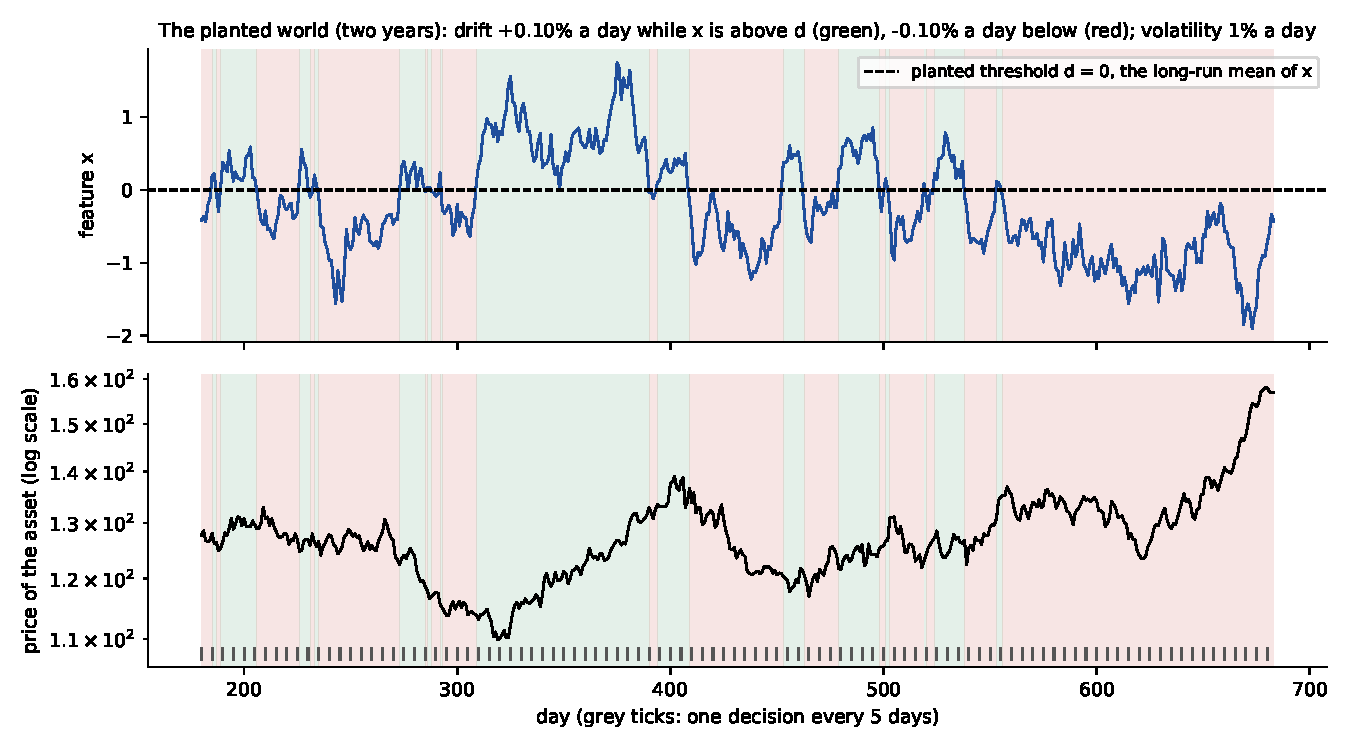
\includegraphics[width=0.95\linewidth]{planted_world_one_dataset}
\caption{Two years of one dataset (base parameters, weekly decisions). The background is the true regime, which the tree never sees; a decision is taken at each grey tick and held until the next one.}
\label{fig:world}
\end{figure}

\section{Protocol}\label{sec:protocol}
\textbf{Pipeline used.} P2 of \code{model_history.md}: the tree of \code{model_and_training_pipeline.tex} with every option off (plain splits, every threshold screened, depth 2, 20 decisions per leaf, pruning on the last quarter of the training decisions, $\lambda=1$, fee 3 bp), with the Sharpe ratio of an all-cash path defined as 0; market M2 (Section~\ref{sec:world}).

For each cell (a trading rate $h$ with an edge $e$, or with a speed $k$ at $e=0.10$) and each of its $N$ independent datasets: simulate 180 + 3{,}780 + 1{,}260 days; fit the tree on the 15 training years; replay it on the 5 test years, starting from its holdings at the end of training. Four benchmarks are replayed on the same rows with the same optimizer: the \emph{ideal rule} (optimizer fed with $\hat c=(g_h(x),0)$, the best possible use of $x$); the \emph{rule at $d$} (scores $\pm10\%$ according to $x\ge d$); \emph{always the asset}; the \emph{tree without splits} (one leaf, i.e.\ no information). Four measurements:
\begin{enumerate}\setlength{\itemsep}{1pt}
\item \textbf{Does it split, and where?} Share of datasets whose first split is on $x$ (with one feature, the alternative is no split); the distribution of the first threshold, whose target is $d=0$ in units of the standard deviation of $x$.
\item \textbf{Test Sharpe ratio}, annualized as $\sqrt{252/h}\times$ the per-decision Sharpe of net returns, averaged over the datasets.
\item \textbf{Share of the possible gain captured}: $(R_{\text{tree}}-R_{\text{flat}})/(R_{\text{ideal}}-R_{\text{flat}})$ with $R$ the mean test return, pooled over the datasets of a cell (blank when the ideal rule gains under 0.5\% a year: nothing to capture).
\item \textbf{No split kept}: share of datasets where pruning left a single leaf.
\end{enumerate}

\section{Results}\label{sec:results}
\subsection{One dataset}
\begin{figure}[H]
\centering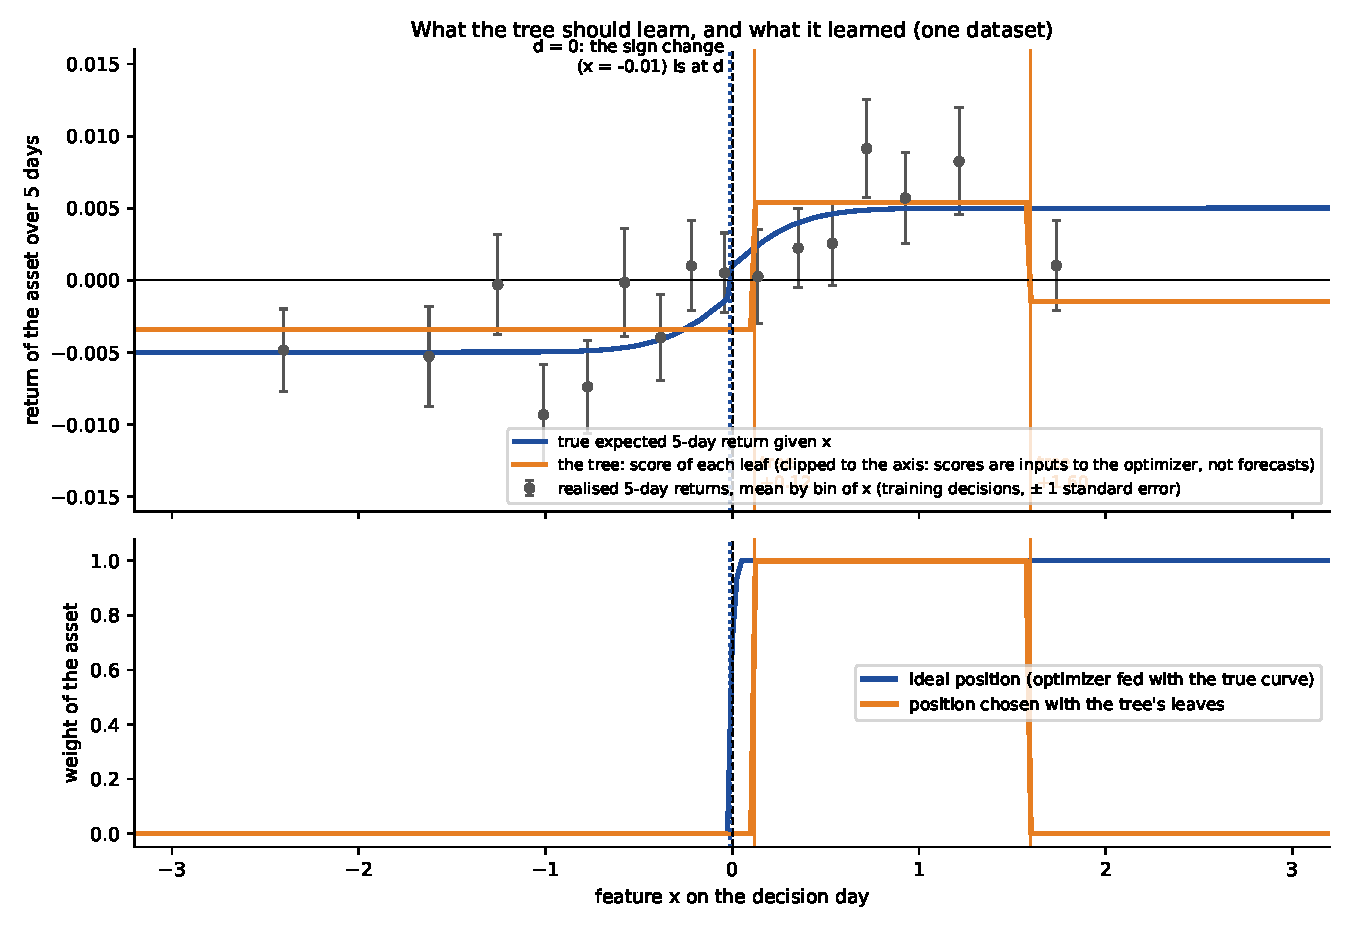
\includegraphics[width=0.95\linewidth]{learned_vs_ideal_one_dataset}
\caption{Base parameters, weekly decisions, dataset 42. \emph{Top:} realised 5-day returns by bin of $x$ (training decisions), the true $g_5(x)$ of \eqref{eq:g}, and the tree's leaf scores. \emph{Bottom:} the position the optimizer takes with the true curve and with the tree. Growth made three splits. Pruning removed the one at $x\le-2.01$ and kept the root split at $x\le0.12$ (on the checking decisions: regret $0.0097\to0.0066$ per decision, Sharpe $0.06\to0.20$) together with a second-level one at $x\le1.60$ (31 decisions, regret $0.0067\to0.0066$), an example of the tail leaves discussed in Section~\ref{sec:says}.}
\label{fig:learned}
\end{figure}
\begin{figure}[H]
\centering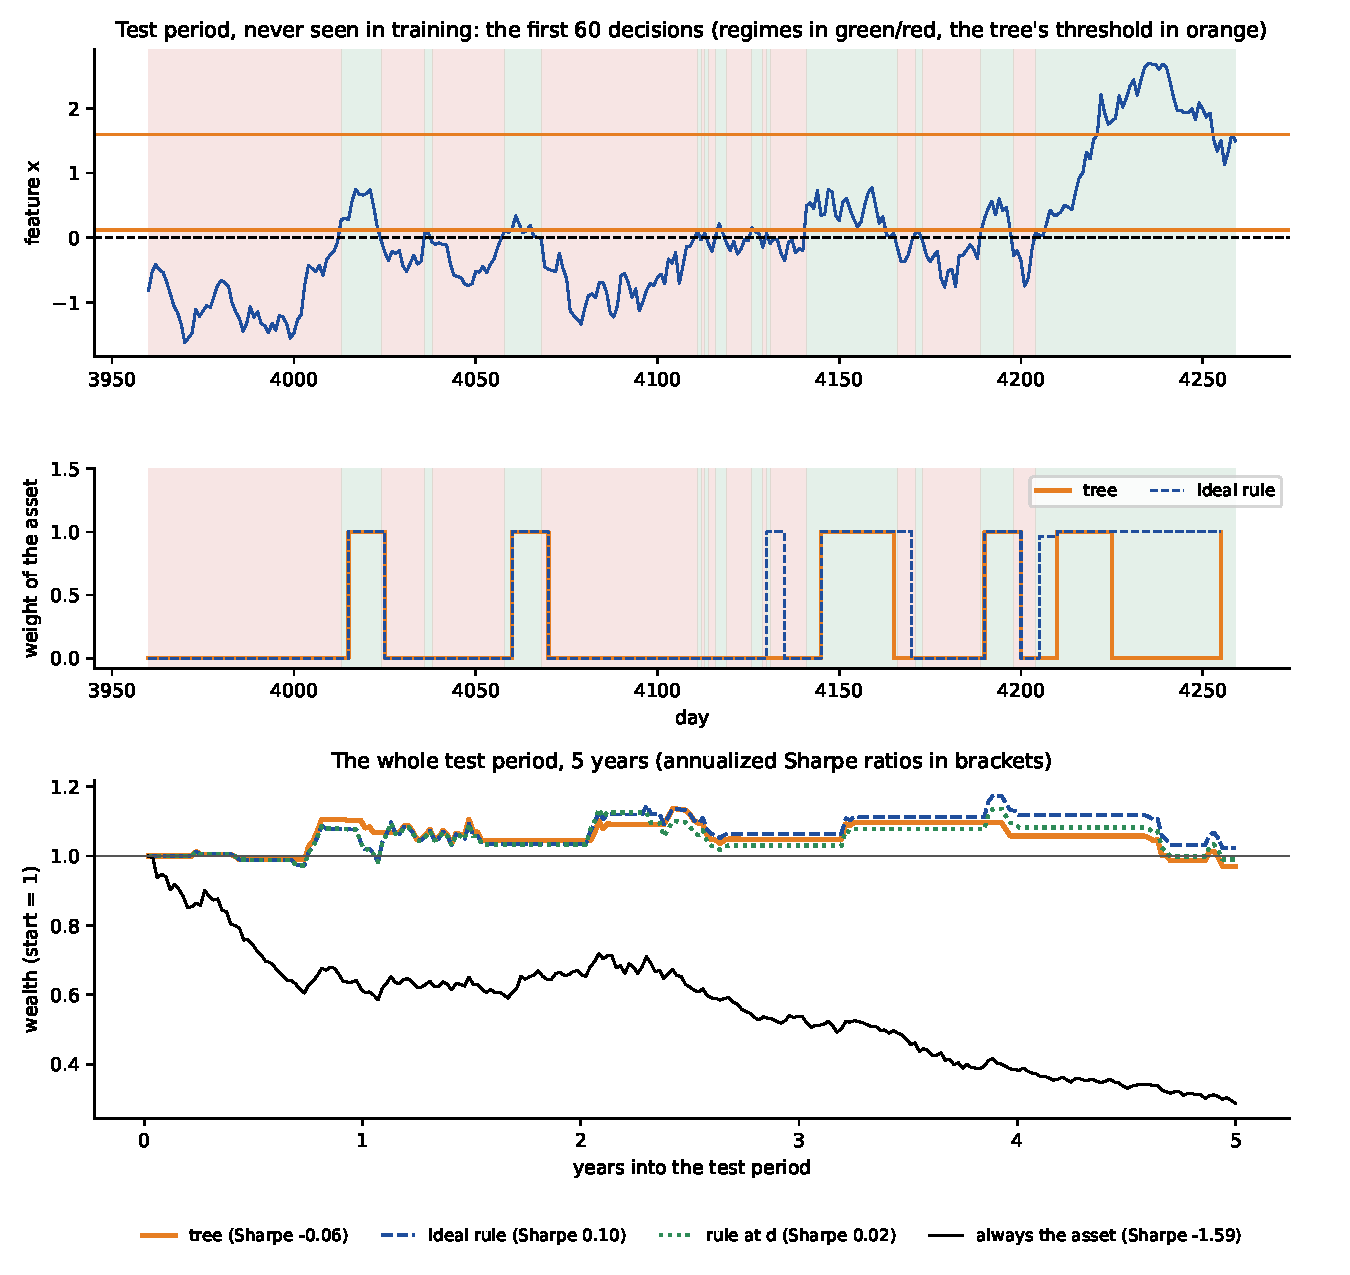
\includegraphics[width=0.95\linewidth]{test_decisions_one_dataset}
\caption{The same dataset out of sample. \emph{Top, middle:} the first 60 test decisions; the tree is in cash below its threshold and fully invested above, like the ideal rule. \emph{Bottom:} wealth over the 5 test years. This test window is dominated by the down regime (the asset loses 22\% a year), so every rule earns little; what the figure shows is the decisions, not the level of the returns.}
\label{fig:decisions}
\end{figure}

\subsection{Where the threshold lands, over 100 datasets per cell}
\begin{figure}[H]
\centering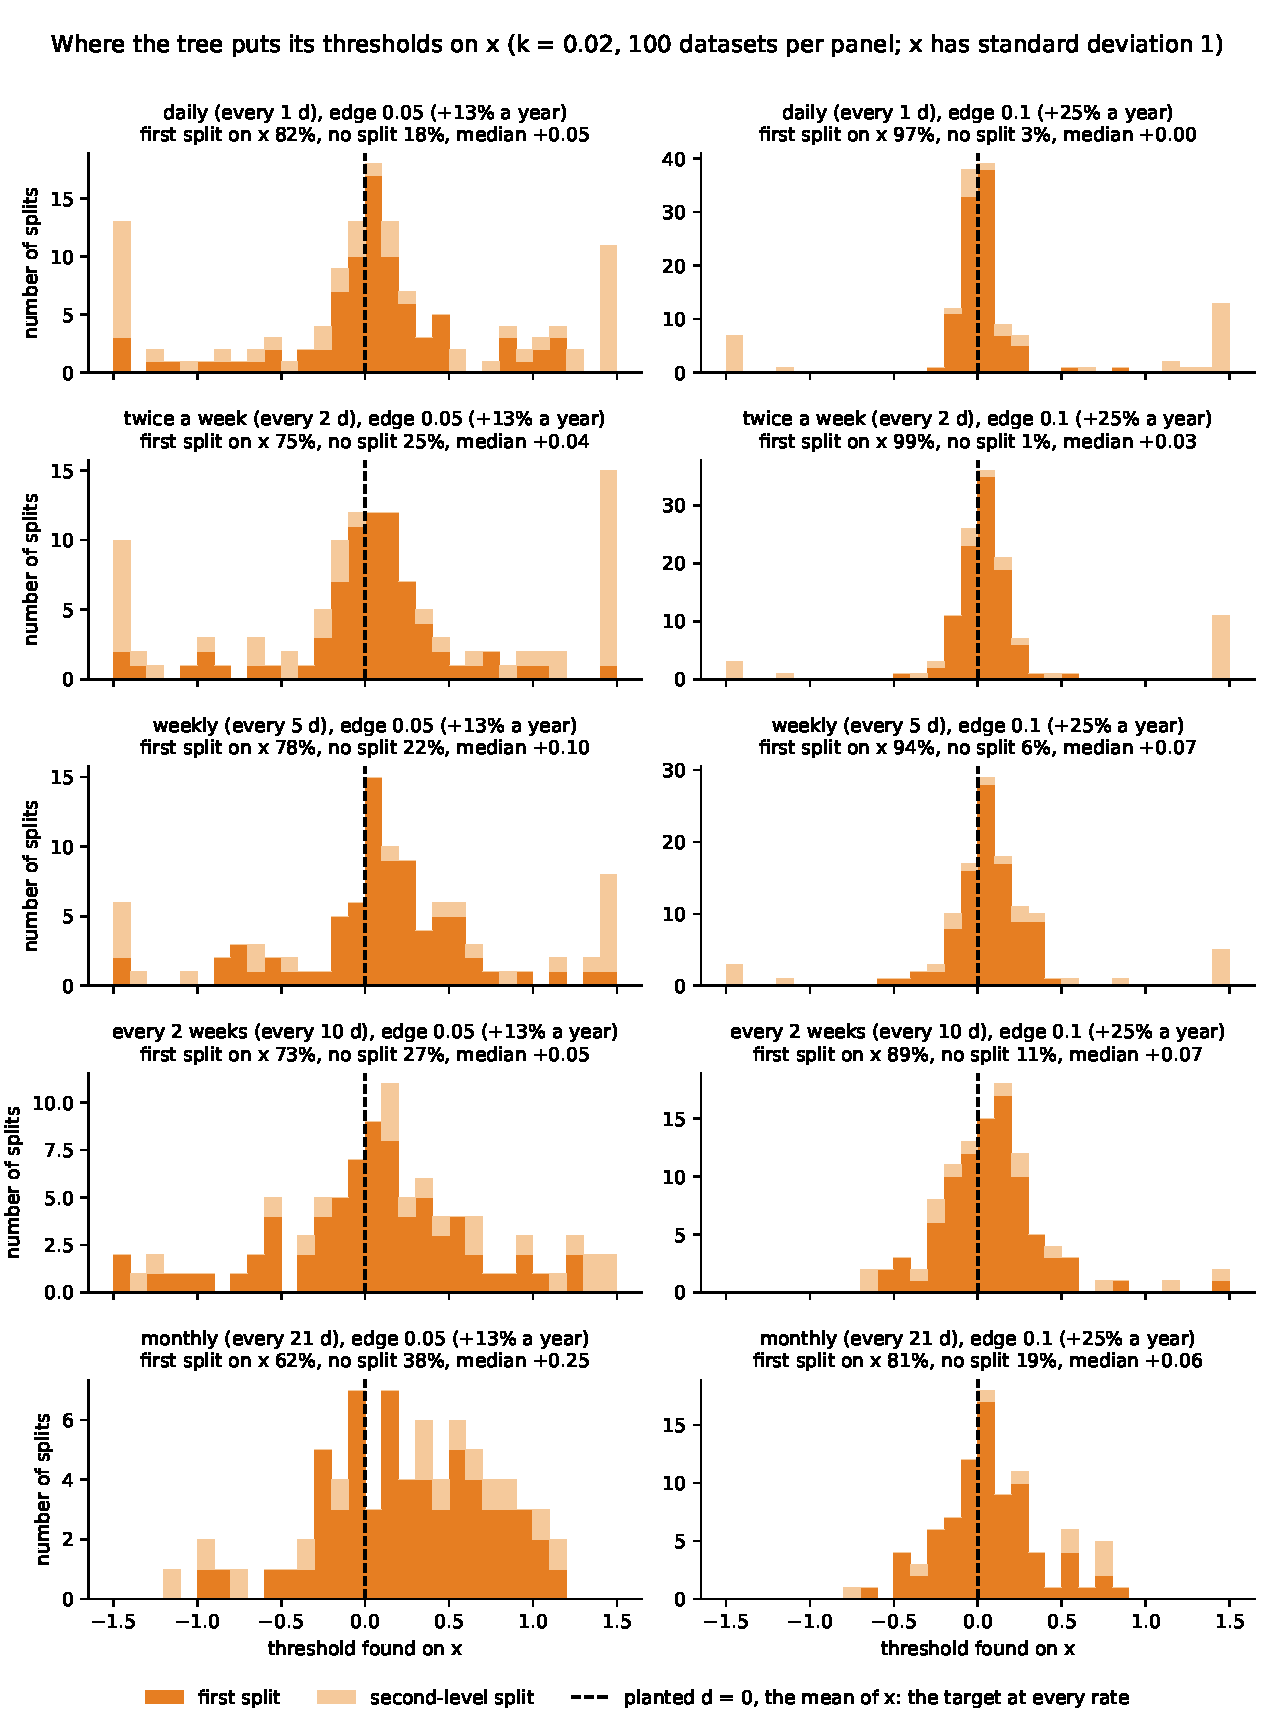
\includegraphics[width=0.92\linewidth]{thresholds_by_rate_histograms}
\caption{All thresholds on $x$ kept in the final trees, one panel per trading rate, $k=0.02$; \emph{top:} edge 0.05, \emph{bottom:} edge 0.10. The target is $d=0$ at every rate; $x$ has standard deviation 1. Bars at $\pm1.5$ collect thresholds beyond the axis (tail leaves).}
\label{fig:hist}
\end{figure}
\begin{figure}[H]
\centering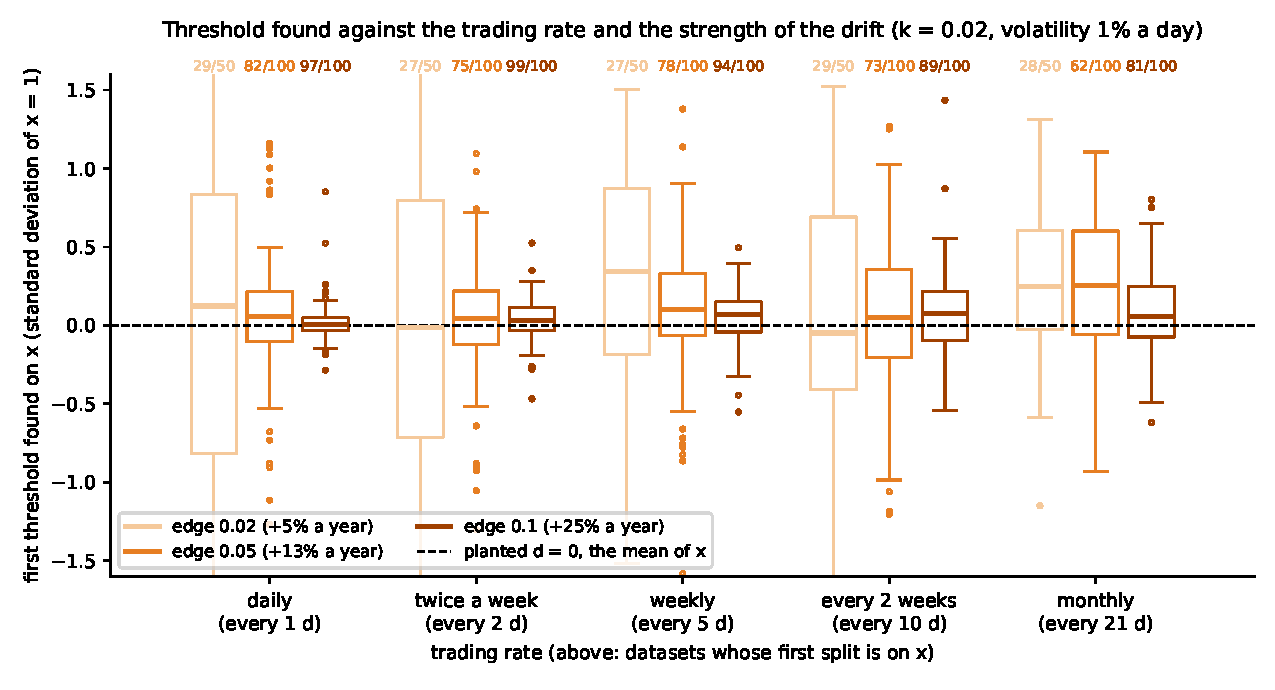
\includegraphics[width=\linewidth]{thresholds_by_rate_boxplots}
\caption{First threshold found, by trading rate and edge (boxes: quartiles; the count above each box is the number of datasets that split).}
\label{fig:byrate}
\end{figure}

\subsection{Trading rate against edge, and against the speed of the feature}
\begin{figure}[H]
\centering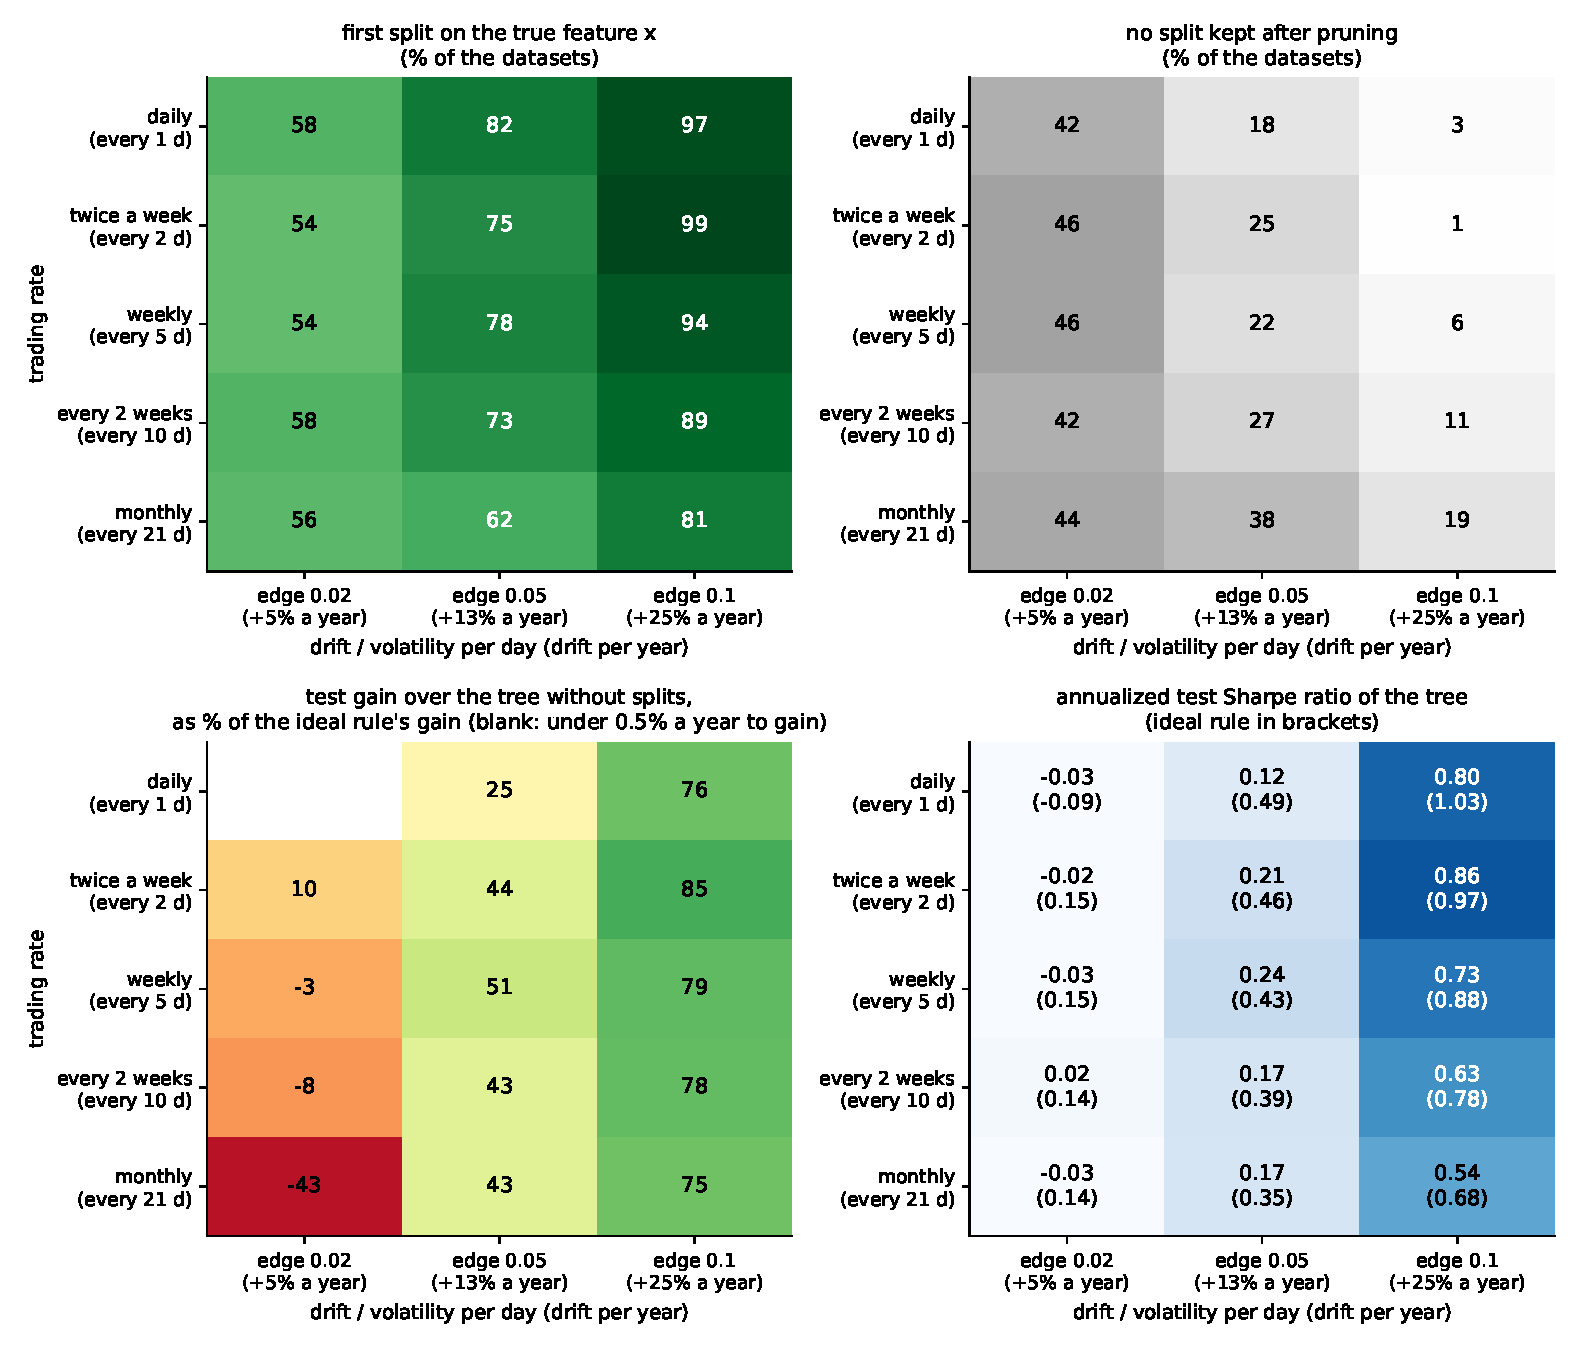
\includegraphics[width=0.95\linewidth]{maps_rate_vs_edge}
\caption{Rows: trading rate; columns: edge ($k=0.02$). From left to right: datasets whose first split is on $x$; datasets that keep no split; share of the ideal rule's test gain captured; annualized test Sharpe ratio of the tree (ideal rule in brackets).}
\label{fig:maps}
\end{figure}
\begin{figure}[H]
\centering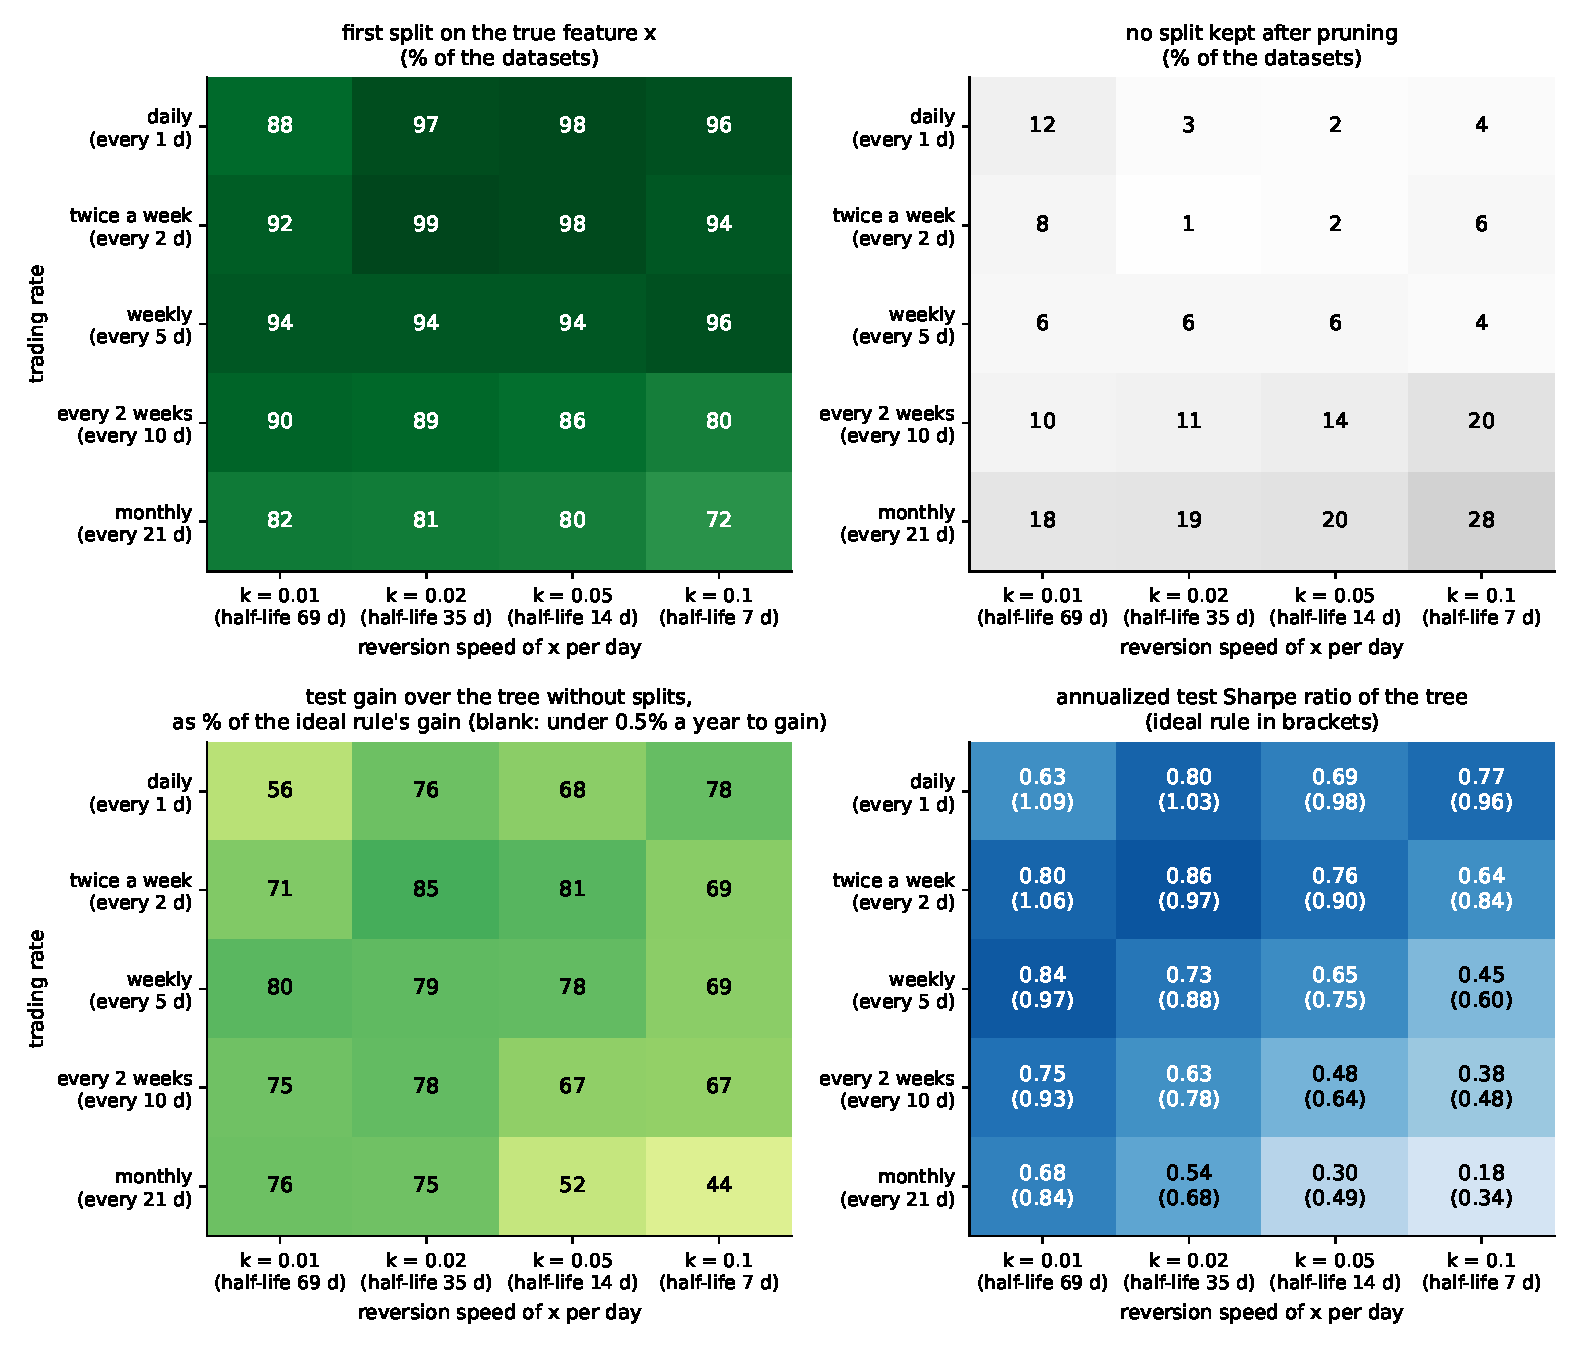
\includegraphics[width=0.95\linewidth]{maps_rate_vs_speed}
\caption{Same maps with the reversion speed of $x$ in columns, at edge 0.10.}
\label{fig:mapsk}
\end{figure}

\begin{table}[H]
\centering\small
\setlength{\tabcolsep}{4.5pt}
\begin{tabular}{@{}l r rr r r rrr r@{}}
\toprule
& & \multicolumn{2}{c}{splits (\%)} & \multicolumn{2}{c}{first threshold on $x$} & \multicolumn{3}{c}{annualized test Sharpe} & gain\\
\cmidrule(lr){3-4}\cmidrule(lr){5-6}\cmidrule(lr){7-9}
edge & $h$ & on $x$ & none & median [quartiles] & $|\cdot|\le0.25$ & tree & ideal & at $d$ & captured\\
\midrule
0.10 & 1 & 97 & 3 & $+0.00\ [-0.03,+0.05]$ & 95\% & 0.80 & 1.03 & 1.04 & 76\%\\
 & 2 & 99 & 1 & $+0.03\ [-0.03,+0.11]$ & 92\% & 0.86 & 0.97 & 0.98 & 85\%\\
 & 5 & 94 & 6 & $+0.07\ [-0.04,+0.15]$ & 81\% & 0.73 & 0.88 & 0.88 & 79\%\\
 & 10 & 89 & 11 & $+0.07\ [-0.10,+0.21]$ & 70\% & 0.63 & 0.78 & 0.78 & 78\%\\
 & 21 & 81 & 19 & $+0.06\ [-0.07,+0.25]$ & 60\% & 0.54 & 0.68 & 0.66 & 75\%\\
\midrule
0.05 & 1 & 82 & 18 & $+0.05\ [-0.10,+0.22]$ & 60\% & 0.12 & 0.49 & 0.49 & 25\%\\
 & 2 & 75 & 25 & $+0.04\ [-0.12,+0.22]$ & 64\% & 0.21 & 0.46 & 0.46 & 44\%\\
 & 5 & 78 & 22 & $+0.10\ [-0.07,+0.33]$ & 53\% & 0.24 & 0.43 & 0.42 & 51\%\\
 & 10 & 73 & 27 & $+0.05\ [-0.20,+0.36]$ & 47\% & 0.17 & 0.39 & 0.38 & 43\%\\
 & 21 & 62 & 38 & $+0.25\ [-0.06,+0.60]$ & 34\% & 0.17 & 0.35 & 0.34 & 43\%\\
\midrule
0.02 & 1 & 58 & 42 & $+0.12\ [-0.82,+0.83]$ & 24\% & $-0.03$ & $-0.09$ & 0.14 & --\\
 & 2 & 54 & 46 & $-0.01\ [-0.71,+0.80]$ & 15\% & $-0.02$ & 0.15 & 0.13 & 10\%\\
 & 5 & 54 & 46 & $+0.34\ [-0.19,+0.87]$ & 26\% & $-0.03$ & 0.15 & 0.13 & $-3$\%\\
 & 10 & 58 & 42 & $-0.05\ [-0.41,+0.69]$ & 24\% & 0.02 & 0.14 & 0.13 & $-8$\%\\
 & 21 & 56 & 44 & $+0.25\ [-0.02,+0.60]$ & 32\% & $-0.03$ & 0.14 & 0.14 & $-43$\%\\
\bottomrule
\end{tabular}
\caption{Trading rate $h$ (days between decisions) against edge, $k=0.02$; 100 datasets per row at edges 0.10 and 0.05, 50 at 0.02. ``Always the asset'' has an annualized Sharpe between $-0.04$ and $0.00$ everywhere (no unconditional drift). Standard error of the tree--ideal Sharpe difference: 0.03 to 0.05.}
\label{tab:edge}
\end{table}

\begin{table}[H]
\centering\small
\setlength{\tabcolsep}{4.5pt}
\begin{tabular}{@{}l r rr r r rr r@{}}
\toprule
& & \multicolumn{2}{c}{splits (\%)} & \multicolumn{2}{c}{first threshold on $x$} & \multicolumn{2}{c}{annualized Sharpe} & gain\\
\cmidrule(lr){3-4}\cmidrule(lr){5-6}\cmidrule(lr){7-8}
half-life of $x$ & $h$ & on $x$ & none & median [quartiles] & $|\cdot|\le0.25$ & tree & ideal & captured\\
\midrule
69 days ($k=0.01$) & 1 & 88 & 12 & $+0.00\ [-0.03,+0.08]$ & 86\% & 0.63 & 1.09 & 56\%\\
 & 2 & 92 & 8 & $+0.05\ [-0.00,+0.08]$ & 89\% & 0.80 & 1.06 & 71\%\\
 & 5 & 94 & 6 & $+0.05\ [-0.04,+0.12]$ & 87\% & 0.84 & 0.97 & 80\%\\
 & 10 & 90 & 10 & $+0.06\ [-0.11,+0.14]$ & 87\% & 0.75 & 0.93 & 75\%\\
 & 21 & 82 & 18 & $+0.15\ [-0.06,+0.23]$ & 71\% & 0.68 & 0.84 & 76\%\\
\midrule
14 days ($k=0.05$) & 1 & 98 & 2 & $+0.00\ [-0.01,+0.06]$ & 94\% & 0.69 & 0.98 & 68\%\\
 & 2 & 98 & 2 & $+0.05\ [-0.01,+0.15]$ & 88\% & 0.76 & 0.90 & 81\%\\
 & 5 & 94 & 6 & $+0.18\ [-0.02,+0.25]$ & 74\% & 0.65 & 0.75 & 78\%\\
 & 10 & 86 & 14 & $+0.21\ [-0.05,+0.43]$ & 44\% & 0.48 & 0.64 & 67\%\\
 & 21 & 80 & 20 & $+0.12\ [-0.16,+0.34]$ & 40\% & 0.30 & 0.49 & 52\%\\
\midrule
7 days ($k=0.10$) & 1 & 96 & 4 & $+0.02\ [-0.02,+0.07]$ & 92\% & 0.77 & 0.96 & 78\%\\
 & 2 & 94 & 6 & $+0.03\ [-0.02,+0.16]$ & 74\% & 0.64 & 0.84 & 69\%\\
 & 5 & 96 & 4 & $+0.17\ [+0.04,+0.45]$ & 52\% & 0.45 & 0.60 & 69\%\\
 & 10 & 80 & 20 & $+0.20\ [-0.14,+0.54]$ & 38\% & 0.38 & 0.48 & 67\%\\
 & 21 & 72 & 28 & $+0.10\ [-0.03,+0.58]$ & 47\% & 0.18 & 0.34 & 44\%\\
\bottomrule
\end{tabular}
\caption{Trading rate against the speed of $x$, at edge 0.10, 50 datasets per row (the 35-day row is the edge-0.10 block of Table~\ref{tab:edge}).}
\label{tab:k}
\end{table}

\textbf{Reading the figures and tables.}
\begin{itemize}\setlength{\itemsep}{1pt}
\item At edge 0.10 the tree splits on $x$ in 81 to 99\% of the datasets and puts its threshold at the mean: median $0.00$ to $0.07$, quartiles within $\pm0.05$ daily and $[-0.07,+0.25]$ monthly. Out of sample it is 0.11 to 0.23 of annual Sharpe below the ideal rule (standard error 0.03--0.04) and captures 75 to 85\% of the gain. The rule at $d$ equals the ideal rule: with these sizes the ideal position is all or nothing.
\item At edge 0.05 the threshold is found in 62 to 82\% of the datasets but with quartiles of about $\pm0.2$, and 25 to 51\% of the gain is captured. At edge 0.02 the thresholds spread over the whole range and no gain is captured; the ideal rule itself reaches a Sharpe of 0.15 at most. Fifteen years of data do not contain that signal.
\item The trading rate matters little from daily to weekly. Every two weeks and monthly lose ground (81\% found and 60\% within $\pm0.25$ at $h=21$ against 97\% and 95\% daily), for two reasons visible in Table~\ref{tab:k}: fewer decisions to learn from (180 monthly ones) and, when $x$ is fast, a regime that flips inside the holding period ($g_{21}(1)=0.87\%$ at $k=0.10$ against $1.79\%$ at $k=0.02$).
\item The slow rates show a small upward bias of the median threshold ($+0.06$ to $+0.25$): with a holding period and fees, entering just above the mean is not worth the trade, so the tree waits for $x$ to be clearly positive.
\item The no-split share rises from 3\% (daily) to 19\% (monthly) at edge 0.10 and reaches 42--46\% at edge 0.02: when the checking decisions do not confirm a split, the tree stays flat, which is the safe side.
\end{itemize}

\section{The first experiment (18 September): a large drift with decoys}\label{sec:first}
\textbf{Pipeline used.} P1: the same tree before the all-cash Sharpe convention (an all-cash path had an undefined Sharpe ratio); market M1, with three decoy features next to $x$.

The first run used the same tree, optimizer and price model, but with a step as the time unit and sizes far from markets: $\mu=3\%$ per step for $\sigma=3.2\%$ per step, an edge of about 0.95 instead of 0.02--0.10. It also placed the threshold \emph{below} the mean of $x$ and hid $x$ among decoys. It is kept here because it answers two questions the new run does not: are decoys ignored, and what does the tree find when $d\neq m$?
\begin{table}[H]
\centering\small
\begin{tabularx}{\linewidth}{@{}l L L@{}}
\toprule
Parameter & Value & Note\\
\midrule
$\mu$, $\sigma$ & 3\%, 3.2\% per step & edge 0.95; volatilities 1 to 30\% per step also swept\\
$d$; $m$, $s^2$ & 0; 1, 4 & $d$ half a standard deviation below the mean: $x\ge d$ 69\% of the time\\
$k$ & 0.2 per step & a regime lasts about 5 steps; 0.01 to 0.5 also swept\\
$h$ & 10 steps (and 1) & a position held while the regime changes twice on average\\
features & $x$, 20-step average of $x$, an unrelated OU with the same law, white noise & three decoys\\
data & 443 training decisions (332 grow, 111 prune), 300 test & 100 datasets per histogram, 20 per cell of the $k\times\sigma$ map, 800 fits\\
\bottomrule
\end{tabularx}
\caption{The first experiment.}
\end{table}
\textbf{What should the tree find when $d\neq m$?} Not $d$. Held for 10 steps, a position taken just below $d$ is soon above it, because $x$ reverts to $m=1>d$. The expected 10-step return $g_{10}$ of \eqref{eq:g} changes sign at $x\approx-0.92$, and the ideal position rises from 0 to 1 between there and about $-0.3$. The right question was ``does the tree put its threshold in $[-0.9,-0.3]$?'', and $d$ itself is the target only for $h=1$.

\textbf{Results.}
\begin{itemize}\setlength{\itemsep}{1pt}
\item $h=1$ (target $d$): first split on $x$ in 100 datasets of 100, one split per tree, never a decoy; median threshold $0.000$, 95 of 100 within $0.1$ of $d$ ($s=2$). Test Sharpe per decision: tree 0.684, ideal rule 0.682, always the asset 0.270.
\item $h=10$ (target $[-0.9,-0.3]$): first split on $x$ in 86 of 100, never first on a decoy, no split in 14; median $-0.46$, 90\% between $-1.53$ and $+0.01$. Test Sharpe per decision: tree 0.724, ideal 0.742, rule at $d$ 0.749, always the asset 0.628 (tree $-0.018\pm0.004$ against the ideal rule). Fifteen trees kept a second split on $x$, three a second-level split on the noise decoy.
\item $k\times\sigma$ map ($h=10$, 600 trees): $x$ is found first in 95--100\% of the datasets when a regime lasts at least about one holding period ($k\le0.1$) and $\sigma\le20\%$; at $k=0.5$ (a regime of 2 steps) in 20--45\%, and then the usual outcome is no split, which is right (the ideal rule gains 0.01\% per decision). Over the 600 trees the noise decoy is the first split in 9 (1.5\%) and the moving average in 30 (5\%), almost all at $\sigma\ge20\%$.
\item The sign change of $g_{10}$ moves with $k$ ($-0.04$, $-0.05$, $-0.16$, $-0.37$, $-0.92$, $-3.6$ for $k=0.01$ to $0.5$) and the tree's median thresholds follow it ($-0.02$, $+0.02$, $-0.04$, $-0.19$, $-0.47$, $-1.52$), staying between the sign change and $d$.
\end{itemize}
\begin{figure}[H]
\centering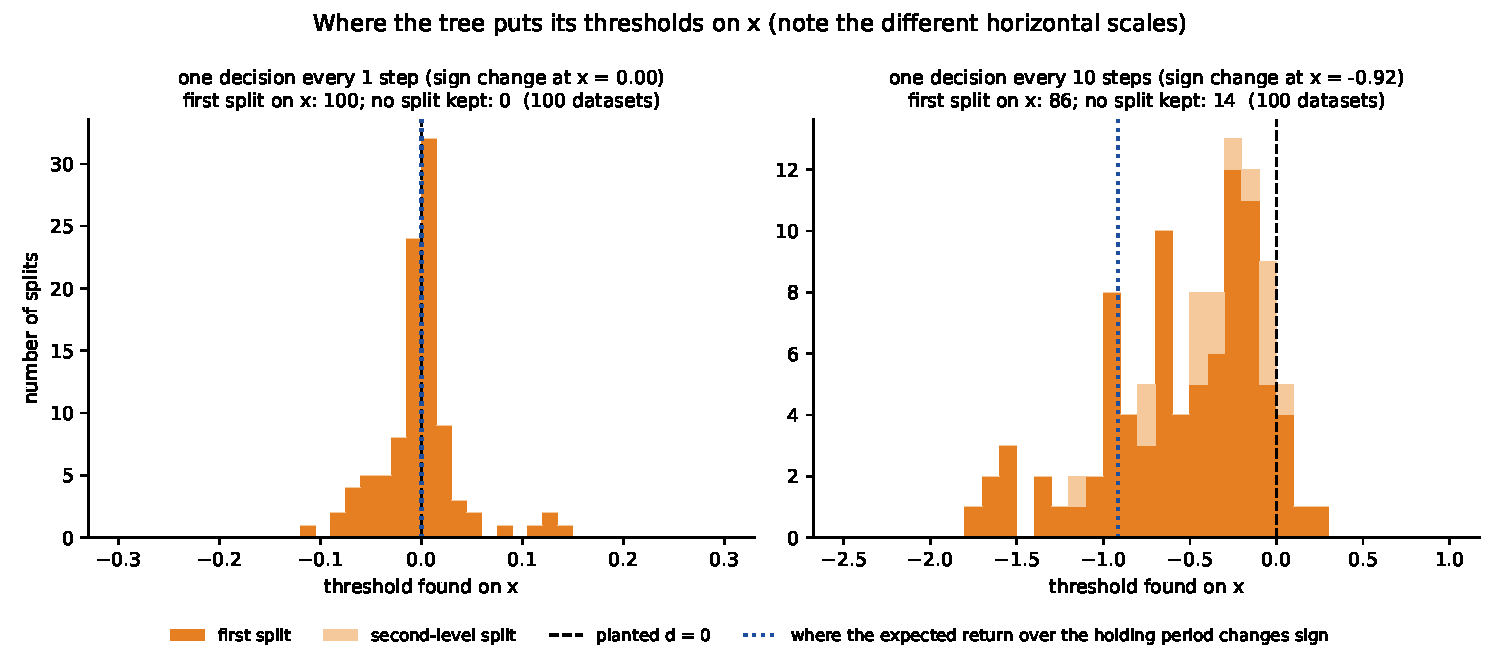
\includegraphics[width=\linewidth]{first_experiment_histograms}
\caption{First experiment: thresholds kept, 100 datasets per panel. \emph{Left:} $h=1$, target $d$. \emph{Right:} $h=10$, target between the sign change (dotted) and about $-0.3$.}
\end{figure}
\begin{figure}[H]
\centering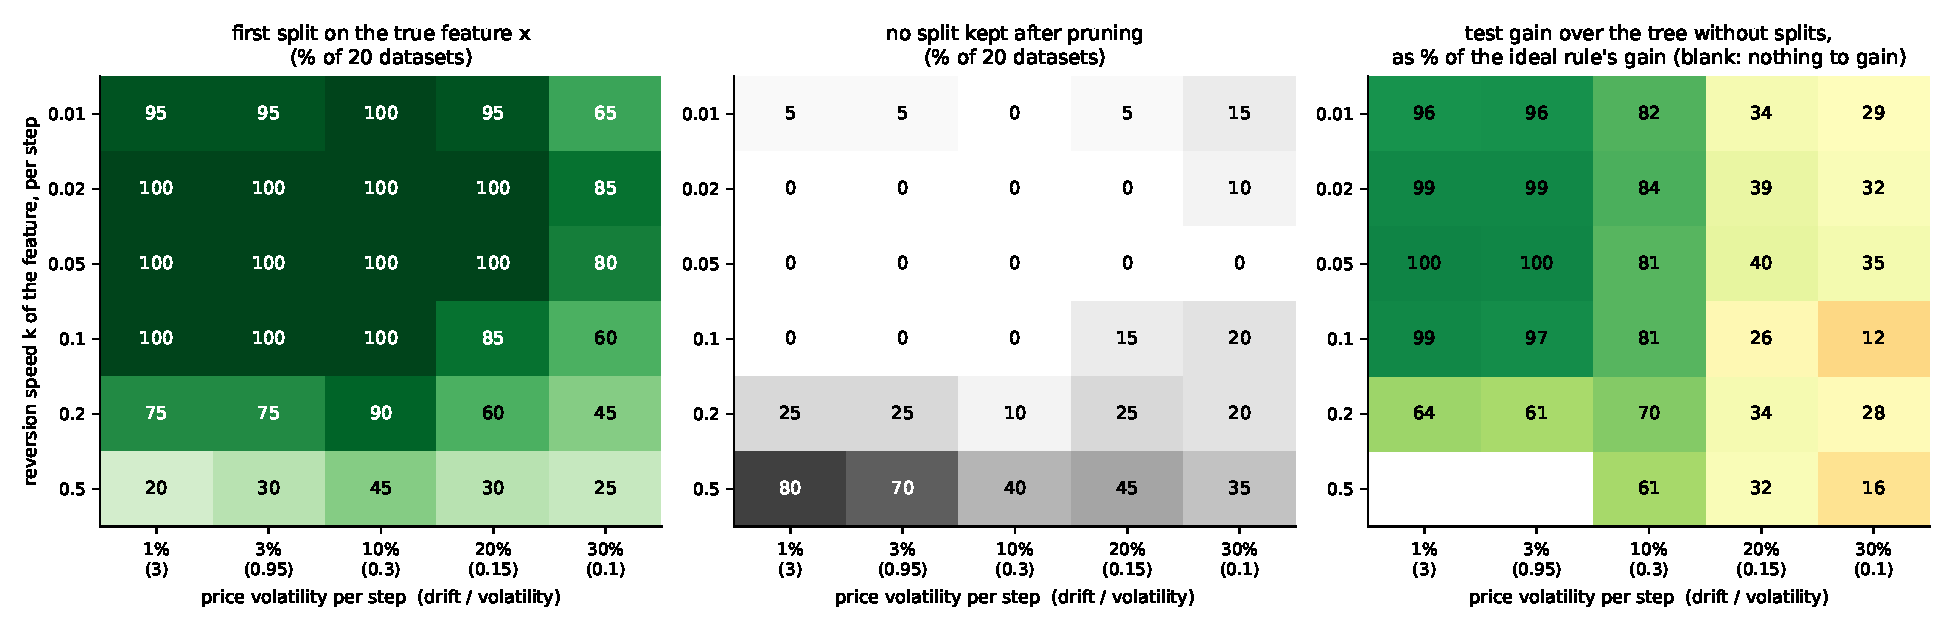
\includegraphics[width=\linewidth]{first_experiment_maps}
\caption{First experiment, $h=10$, 20 datasets per cell: rows are the speed $k$ of $x$, columns the volatility of the price (edge in brackets).}
\end{figure}
\textbf{Why it was not enough.} An edge of 0.95 means the regime is visible in a handful of decisions; the experiments of the main report on real data worked near 0.07. The present run repeats the test at 0.02--0.10, which is what connects it to markets.

\section{What changed in the code}\label{sec:code}
\begin{itemize}\setlength{\itemsep}{1pt}
\item \code{planted_threshold_test.py}: the time unit is the trading day (252 a year); the tree sees $x$ alone; $d=m$; the training and test spans are given in days (15 and 5 years), so that every trading rate sees the same history; the drift is given as an edge $e=\mu/\sigma$; results are annualized by $252/h$.
\item \code{planted_threshold_experiments.py}: the sweeps are trading rate $\times$ edge and trading rate $\times$ speed; the maps carry the annualized Sharpe ratios; a summary table is printed by \code{plot}.
\item \code{spo_tree.py}, one definition: the Sharpe ratio of a path with fewer than two periods stays undefined, but a path with constant zero net returns (all cash, no trade) now has a Sharpe ratio of $0$ instead of NaN. Every comparison ``$\text{Sharpe}_{\text{with split}}>\text{Sharpe}_{\text{without}}$'' was false when the tree without the split sat in cash, so pruning removed every such split, however good; with a zero-mean asset this happened in most datasets. A unit test covers it.
\end{itemize}

\section{What this test says, and what it does not}\label{sec:says}
\begin{itemize}\setlength{\itemsep}{1pt}
\item \textbf{The mechanism works at market sizes.} With a regime drift of $\pm25\%$ a year and a feature that persists for a month, the tree recovers the planted threshold at every trading rate and delivers most of the attainable Sharpe ratio out of sample. At $\pm13\%$ it degrades gracefully; at $\pm5\%$ it correctly finds nothing.
\item \textbf{Deciding more often does not teach more about a slow signal} (daily to weekly are equivalent), but deciding too rarely loses the fast part of the signal and the number of decisions to learn from.
\item \textbf{Tail leaves.} With 3{,}780 daily rows the minimum of 20 decisions per leaf is 0.7\% of the data, and pruning lets some second-level splits in the tails through (the bars at $\pm1.5$ of Figure~\ref{fig:hist}); they cost little here but the minimum leaf size should scale with the number of rows.
\item \textbf{Not shown:} decoys at these edges, an unconditional premium of the asset, several assets, a regime depending on more than one threshold, volatility that changes with the regime.
\end{itemize}


\section{A second experiment: risk aversion, fees, depth and quantile thresholds}\label{sec:settings}
\textbf{Pipeline used.} P2 with $\lambda$, the fee and the depth varied as listed; the ``quartiles'' setting used the quantiles of the node's \emph{values} as candidates, the rule in force on 22 September, not the rank rule of Section~\ref{sec:enhancements}.

\textbf{Why.} The positions of Section~\ref{sec:results} are 0 or 1. With the fee $f$ on the asset and holdings $u$, the optimizer \eqref{eq:opt} gives
\begin{equation}\label{eq:w}
w=\frac{\hat c\mp f}{2\lambda\sigma_h^2}\quad\text{clipped to }[0,1],\qquad\text{and } w=u \text{ inside the no-trade zone } |\hat c-2\lambda\sigma_h^2u|\le f,
\end{equation}
so a position is interior only for scores within a window of width $2\lambda\sigma_h^2$: 0.1\% at weekly decisions with $\lambda=1$, against expected returns of $\pm0.5\%$. The ideal position is then a step, and a step is what the tree learns. To see whether the tree can learn a \emph{gradual} position, and how fees, depth and the number of candidate thresholds change the picture, the same world was run again with one or two things changed at a time (Table~\ref{tab:settings-def}): 40 datasets per cell, edges 0.05 and 0.10, $k=0.02$, decisions every 2, 5, 10 and 21 days (daily decisions were left out: two thirds of the compute for the same result as every 2 days in Section~\ref{sec:results}). One measurement is new: the mean weight taken on the test decisions, by bin of $x$ (Figure~\ref{fig:positions}).
\begin{table}[H]
\centering\small
\begin{tabularx}{\linewidth}{@{}l L@{}}
\toprule
Setting & What changes with respect to the run of Section~\ref{sec:results} (\code{base})\\
\midrule
depth 3 & up to 8 leaves instead of 4\\
$\lambda=5$, depth 3 & risk aversion 5: the window of \eqref{eq:w} is 0.5\% wide at weekly decisions\\
$\lambda=10$, depth 3 & risk aversion 10: window 1\% wide; the ideal position never exceeds one half\\
fee 10 bp & fee 10 basis points per trade instead of 3\\
quartiles, depth 3 & only three candidate thresholds per split, the quartiles of the node's values (\code{threshold_quantiles=(0.25,0.5,0.75)}); every leaf then holds at least a quarter of its parent\\
\bottomrule
\end{tabularx}
\caption{The settings experiment. The settings are fields of \code{Case} (\code{risk_aversion}, \code{fee}, \code{max_depth}, \code{threshold_quantiles}); their defaults reproduce Section~\ref{sec:results}.}
\label{tab:settings-def}
\end{table}

\begin{figure}[H]
\centering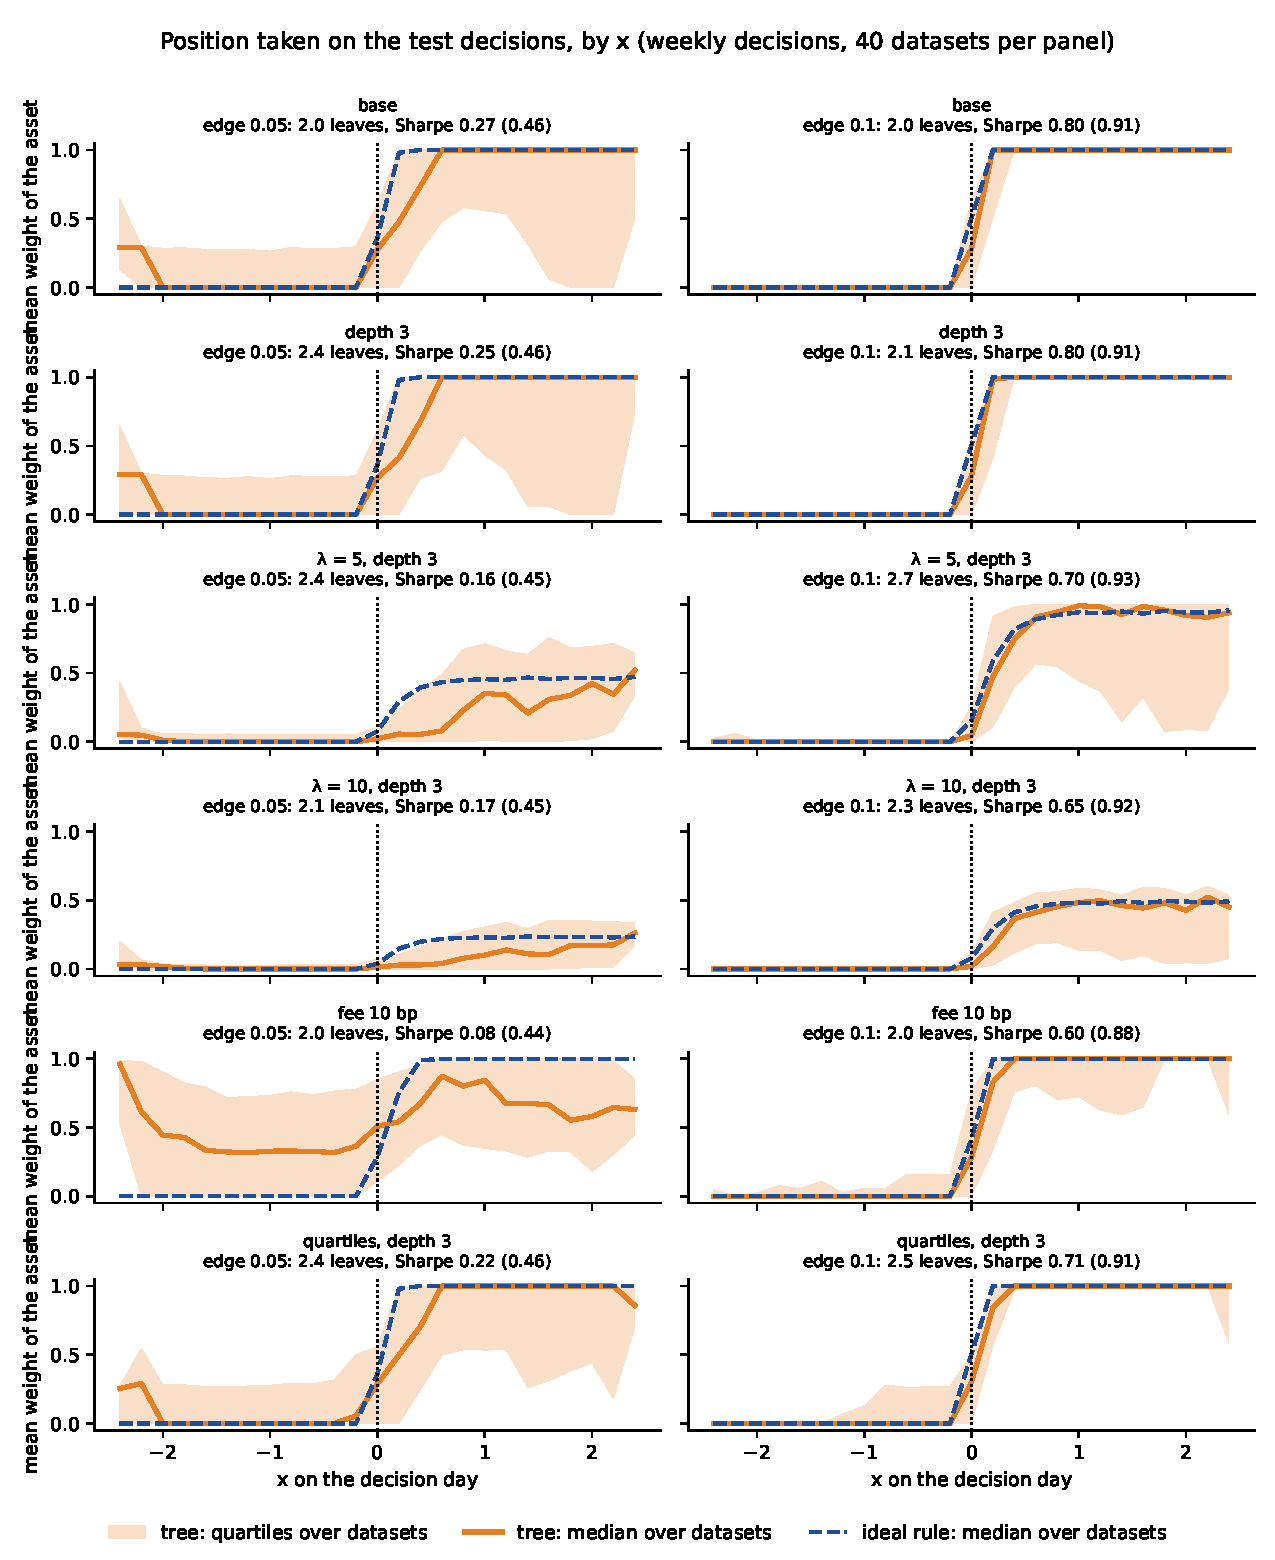
\includegraphics[width=0.85\linewidth]{risk_fee_depth_positions}
\caption{Weekly decisions: the weight of the asset taken on the test decisions, by $x$ on the decision day. Orange: the tree (median over the 40 datasets, and the quartiles as a band); dashed blue: the ideal rule, the optimizer fed with the true $g_5(x)$. One row per setting; \emph{left:} edge 0.05, \emph{right:} edge 0.10. Panel titles: mean number of leaves, annualized test Sharpe ratio of the tree (ideal rule in brackets).}
\label{fig:positions}
\end{figure}
\begin{figure}[H]
\centering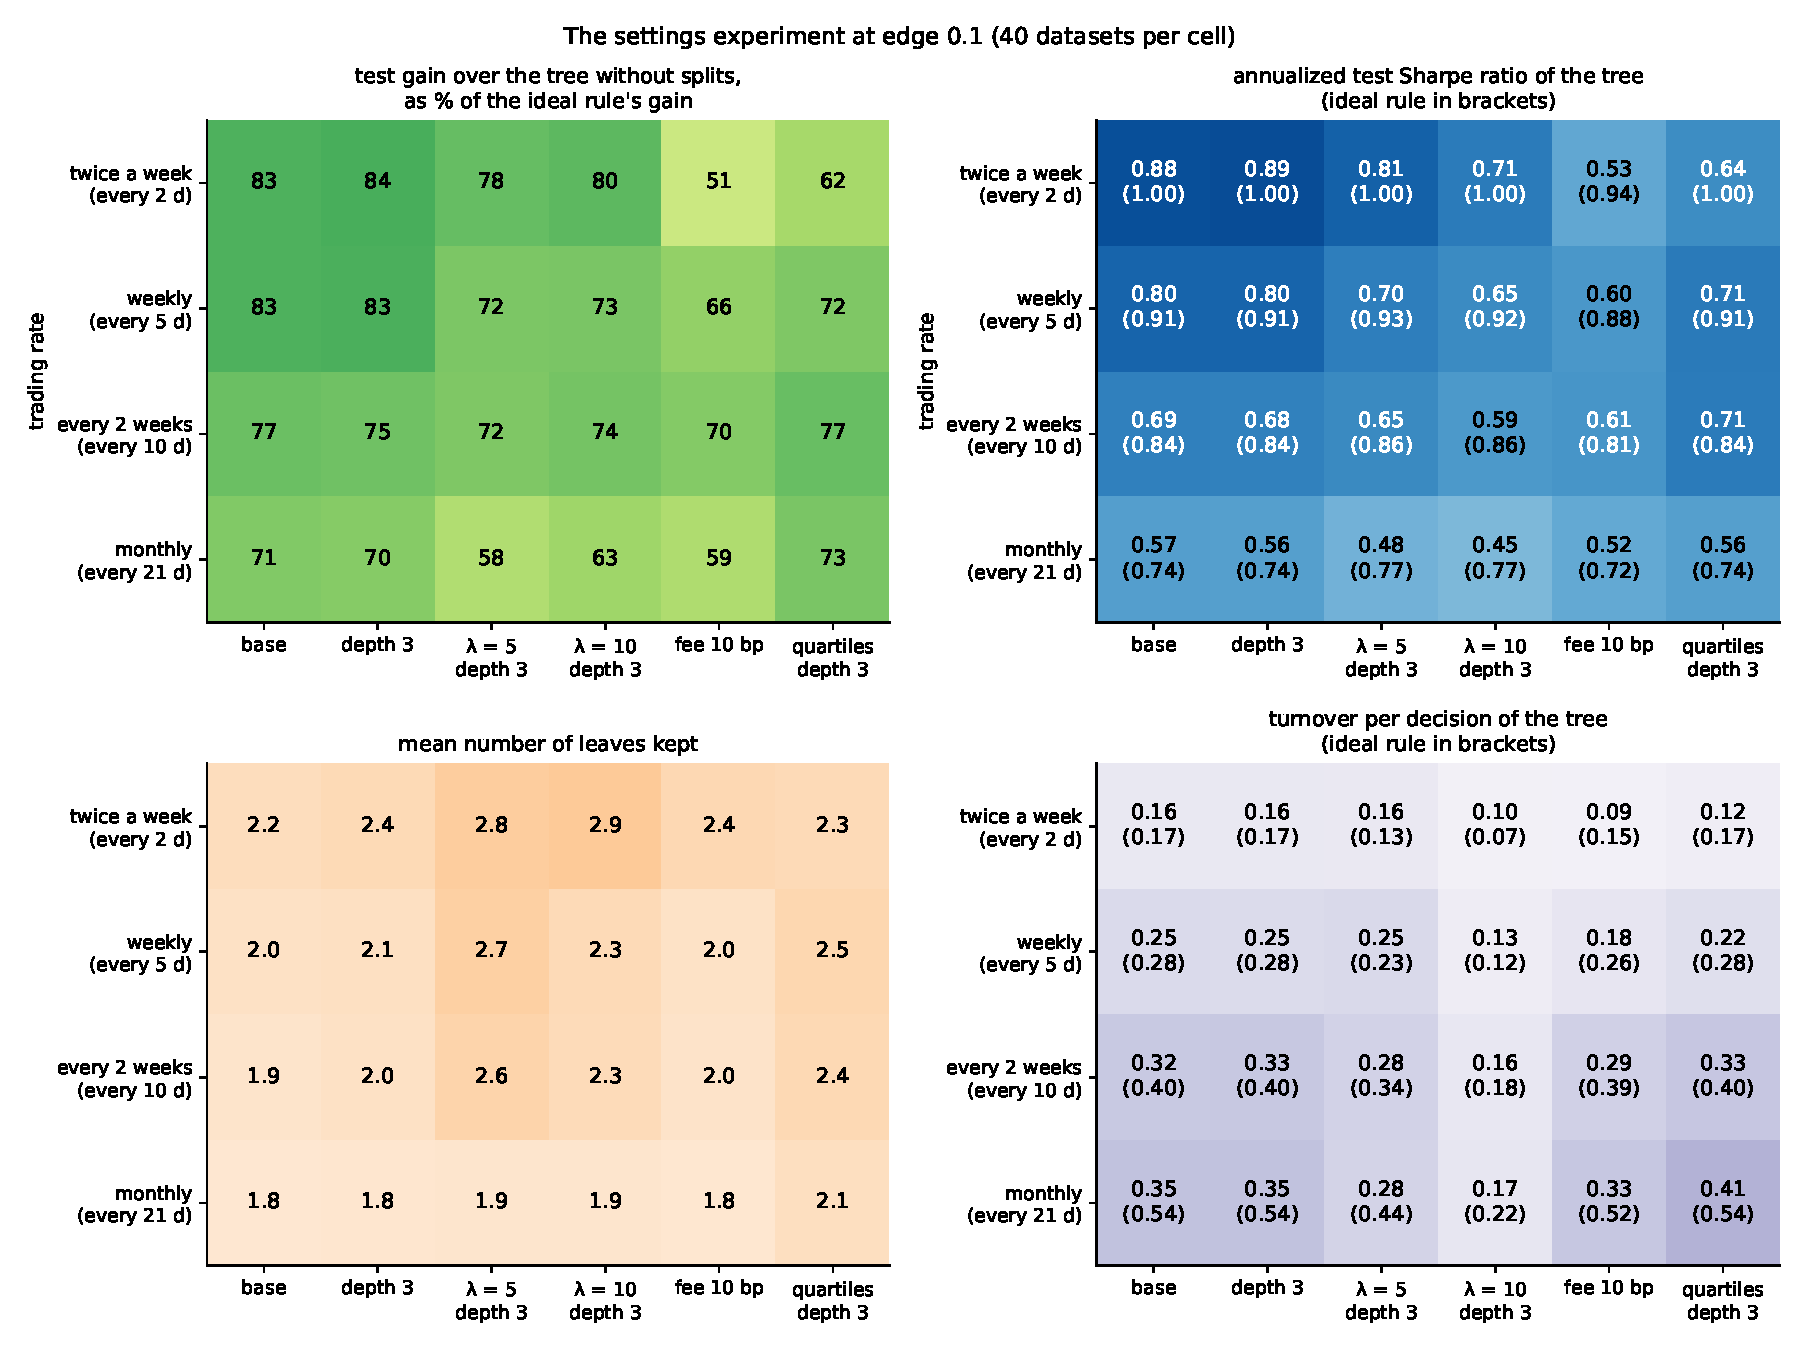
\includegraphics[width=0.95\linewidth]{risk_fee_depth_maps}
\caption{Edge 0.10, rows: trading rate, columns: setting. Share of the ideal rule's test gain captured; annualized test Sharpe ratio (ideal rule in brackets); mean number of leaves kept; turnover per decision (ideal rule in brackets).}
\label{fig:settings-maps}
\end{figure}

\begin{table}[H]
\centering\small
\setlength{\tabcolsep}{4pt}
\begin{tabular}{@{}l r r rr r rr r rr@{}}
\toprule
& & & \multicolumn{2}{c}{splits (\%)} & threshold & \multicolumn{2}{c}{annual.\ Sharpe} & gain & \multicolumn{2}{c}{turnover}\\
\cmidrule(lr){4-5}\cmidrule(lr){7-8}\cmidrule(lr){10-11}
setting & $h$ & leaves & on $x$ & none & median & tree & ideal & captured & tree & ideal\\
\midrule
base & 2 & 2.2 & 98 & 2 & $+0.03$ & 0.88 & 1.00 & 83\% & 0.16 & 0.17\\
 & 5 & 2.0 & 92 & 8 & $+0.08$ & 0.80 & 0.91 & 83\% & 0.25 & 0.28\\
 & 10 & 1.9 & 88 & 12 & $+0.05$ & 0.69 & 0.84 & 77\% & 0.32 & 0.40\\
 & 21 & 1.8 & 72 & 28 & $+0.09$ & 0.57 & 0.74 & 71\% & 0.35 & 0.54\\
\midrule
depth 3 & 2 & 2.4 & 98 & 2 & $+0.03$ & 0.89 & 1.00 & 84\% & 0.16 & 0.17\\
 & 5 & 2.1 & 92 & 8 & $+0.08$ & 0.80 & 0.91 & 83\% & 0.25 & 0.28\\
 & 10 & 2.0 & 88 & 12 & $+0.05$ & 0.68 & 0.84 & 75\% & 0.33 & 0.40\\
 & 21 & 1.8 & 72 & 28 & $+0.09$ & 0.56 & 0.74 & 70\% & 0.35 & 0.54\\
\midrule
$\lambda=5$, depth 3 & 2 & 2.8 & 88 & 12 & $+0.12$ & 0.81 & 1.00 & 78\% & 0.16 & 0.13\\
 & 5 & 2.7 & 82 & 18 & $+0.23$ & 0.70 & 0.93 & 72\% & 0.25 & 0.23\\
 & 10 & 2.6 & 80 & 20 & $+0.26$ & 0.65 & 0.86 & 72\% & 0.28 & 0.34\\
 & 21 & 1.9 & 68 & 32 & $+0.43$ & 0.48 & 0.77 & 58\% & 0.28 & 0.44\\
\midrule
$\lambda=10$, depth 3 & 2 & 2.9 & 85 & 15 & $+0.18$ & 0.71 & 1.00 & 80\% & 0.10 & 0.07\\
 & 5 & 2.3 & 75 & 25 & $+0.25$ & 0.65 & 0.92 & 73\% & 0.13 & 0.12\\
 & 10 & 2.3 & 78 & 22 & $+0.28$ & 0.59 & 0.86 & 74\% & 0.16 & 0.18\\
 & 21 & 1.9 & 70 & 30 & $+0.44$ & 0.45 & 0.77 & 63\% & 0.17 & 0.22\\
\midrule
fee 10 bp & 2 & 2.4 & 95 & 5 & $+0.06$ & 0.53 & 0.94 & 51\% & 0.09 & 0.15\\
 & 5 & 2.0 & 85 & 15 & $+0.08$ & 0.60 & 0.88 & 66\% & 0.18 & 0.26\\
 & 10 & 2.0 & 85 & 15 & $+0.09$ & 0.61 & 0.81 & 70\% & 0.29 & 0.39\\
 & 21 & 1.8 & 68 & 32 & $+0.09$ & 0.52 & 0.72 & 59\% & 0.33 & 0.52\\
\midrule
quartiles, depth 3 & 2 & 2.3 & 92 & 8 & $+0.06$ & 0.64 & 1.00 & 62\% & 0.12 & 0.17\\
 & 5 & 2.5 & 85 & 15 & $+0.09$ & 0.71 & 0.91 & 72\% & 0.22 & 0.28\\
 & 10 & 2.4 & 92 & 8 & $+0.09$ & 0.71 & 0.84 & 77\% & 0.33 & 0.40\\
 & 21 & 2.1 & 80 & 20 & $+0.06$ & 0.56 & 0.74 & 73\% & 0.41 & 0.54\\
\bottomrule
\end{tabular}
\caption{The settings experiment at edge 0.10, 40 datasets per row ($h$: days between decisions). ``Leaves'': mean number of leaves kept; ``median'': first threshold on $x$ over the datasets that split. At edge 0.05 no setting beats the base: the tree's Sharpe ratio is 0.19--0.27 for the base and 0.12--0.19 with $\lambda=5$ or 10, and with a 10 bp fee the tree hardly trades at the fast rates (0.08--0.09).}
\label{tab:settings}
\end{table}

\textbf{Reading the figures and the table.}
\begin{itemize}\setlength{\itemsep}{1pt}
\item \textbf{Depth alone changes nothing}: same leaves, same thresholds, same Sharpe ratios as the base to the second decimal. With $\lambda=1$ the ideal position is a step and the tree has no reason to use more leaves.
\item \textbf{With $\lambda=5$ or 10 the ideal position is a ramp} (to a plateau of one half at $\lambda=10$) \textbf{and the tree follows it}, with 2.3 to 2.9 leaves: it does learn a gradual position when the decision problem asks for one (Figure~\ref{fig:positions}, bottom row). The price is estimation: 72 to 80\% of the gain captured against 83\%, a Sharpe ratio 0.1 to 0.15 lower, thresholds that move up ($+0.12$ to $+0.44$) and more datasets without a split. The ideal rule itself gains nothing from sizing at these signal sizes (its Sharpe ratio is the same at $\lambda=1$, 5 and 10), so a bang-bang position is not a limitation of the tree here; it is what the problem asks for.
\item \textbf{A higher fee does not make positions gradual}: they stay at 0 or 1 with a wider no-trade zone, as \eqref{eq:w} says. Turnover falls (0.09 to 0.33 per decision) and so does everything else: Sharpe 0.52--0.61 against 0.57--0.88 for the base, and at edge 0.05 the tree stops trading at the fast rates.
\item \textbf{Quartile candidates trade precision for stability.} At the fast rates the threshold is less precise (62\% of the gain captured at every 2 days, against 83\%): the candidates are quantiles of a persistent feature, and over the 11 fitting years the sample median of $x$ is itself off by about $\pm0.2$ (autocorrelation time $1/k=50$ days), whereas the full search reads the threshold off the returns. At the slow rates, where the data cannot do better anyway, the coarse grid costs nothing (73\% against 71\% monthly) and its protection against small leaves shows: 20\% of the monthly trees keep no split against 28\%, and the thresholds' medians are the closest to $d$ of all settings ($+0.06$ to $+0.09$).
\end{itemize}


\section{A third experiment: quantile candidates, refinement and soft splits}\label{sec:enhancements}
\textbf{Pipeline used.} P3b: the four split-search options of \code{model_and_training_pipeline.tex} (Section~8 there), the deciles taken by rank among the admissible thresholds; a first run with the deciles of the values (P3) gave the same picture and was replaced by this one.

\textbf{Why.} Sections~\ref{sec:results} and~\ref{sec:settings} showed two sources of error: the threshold moves by $\pm0.1$ to $\pm0.3$ from one dataset to the next, and a split on a handful of decisions occasionally survives pruning. Three options were added to the split search, all off by default (the training document \code{model_and_training_pipeline.tex}, Section~8, gives the exact rules):
\begin{itemize}\setlength{\itemsep}{1pt}
\item \emph{Quantile candidates}: only nine candidates are screened, the deciles \emph{by rank} of the admissible thresholds (those leaving at least the leaf minimum on each side), so they are evenly spread over what is allowed and never on its boundary; and every child keeps at least 10\% of its node. (Quantiles of the node's \emph{values} would differ only at the two ends: their outermost candidates sit on the smallest allowed leaves; see \code{model_and_training_pipeline.tex}, Section~8.)
\item \emph{Refinement}: every partition between the two deciles neighbouring the best one is screened as well; with plain splits the refined threshold wins only if it beats the decile by one standard error of the regret difference;
\item \emph{Soft splits (smoothing $\kappa=1$)}: every candidate threshold $\theta$ keeps a Boltzmann weight $\pi_\theta\propto e^{-z_\theta/\kappa}$, $z_\theta$ its regret excess over the best candidate in standard errors; a decision at $x$ belongs to the left leaf with the weight of the thresholds at or above $x$, so the tree's score becomes a continuous function of $x$ and thresholds the data cannot tell apart share the weight.
\end{itemize}
Each option was run alone and all three together, with the world and the protocol of Section~\ref{sec:settings} (rates 2, 5, 10 and 21 days, edges 0.05 and 0.10, 40 datasets per cell, $\lambda=1$). Two measurements are new: the tree's score as a function of $x$ (Figure~\ref{fig:scores}) and the \emph{spread} of a soft root split, the distance between the 25\% and 75\% quantiles of its weights.

\begin{figure}[H]
\centering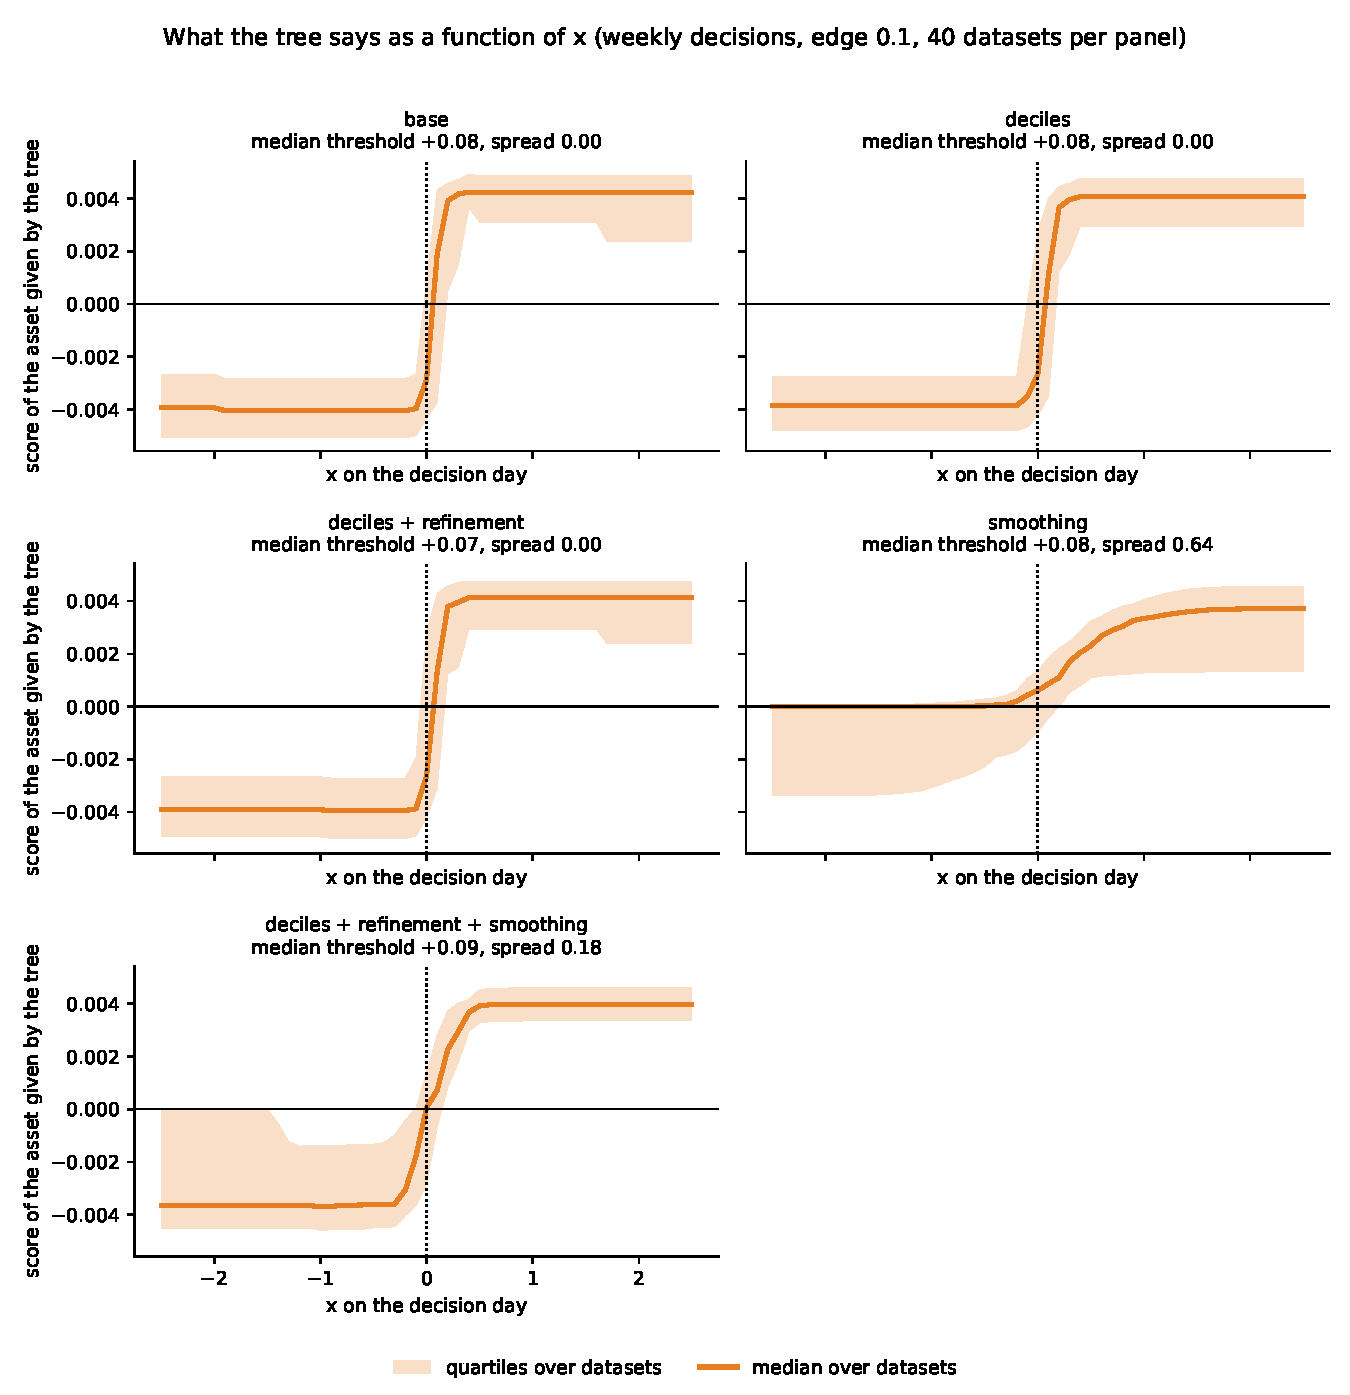
\includegraphics[width=0.9\linewidth]{split_options_scores}
\caption{Weekly decisions, edge 0.10: the score the tree gives the asset as a function of $x$ (median over the 40 datasets, quartiles as a band). Plain splits give a step; smoothing alone gives a ramp that stays near zero over half a standard deviation; the combination gives a step with a narrow soft edge.}
\label{fig:scores}
\end{figure}
\begin{figure}[H]
\centering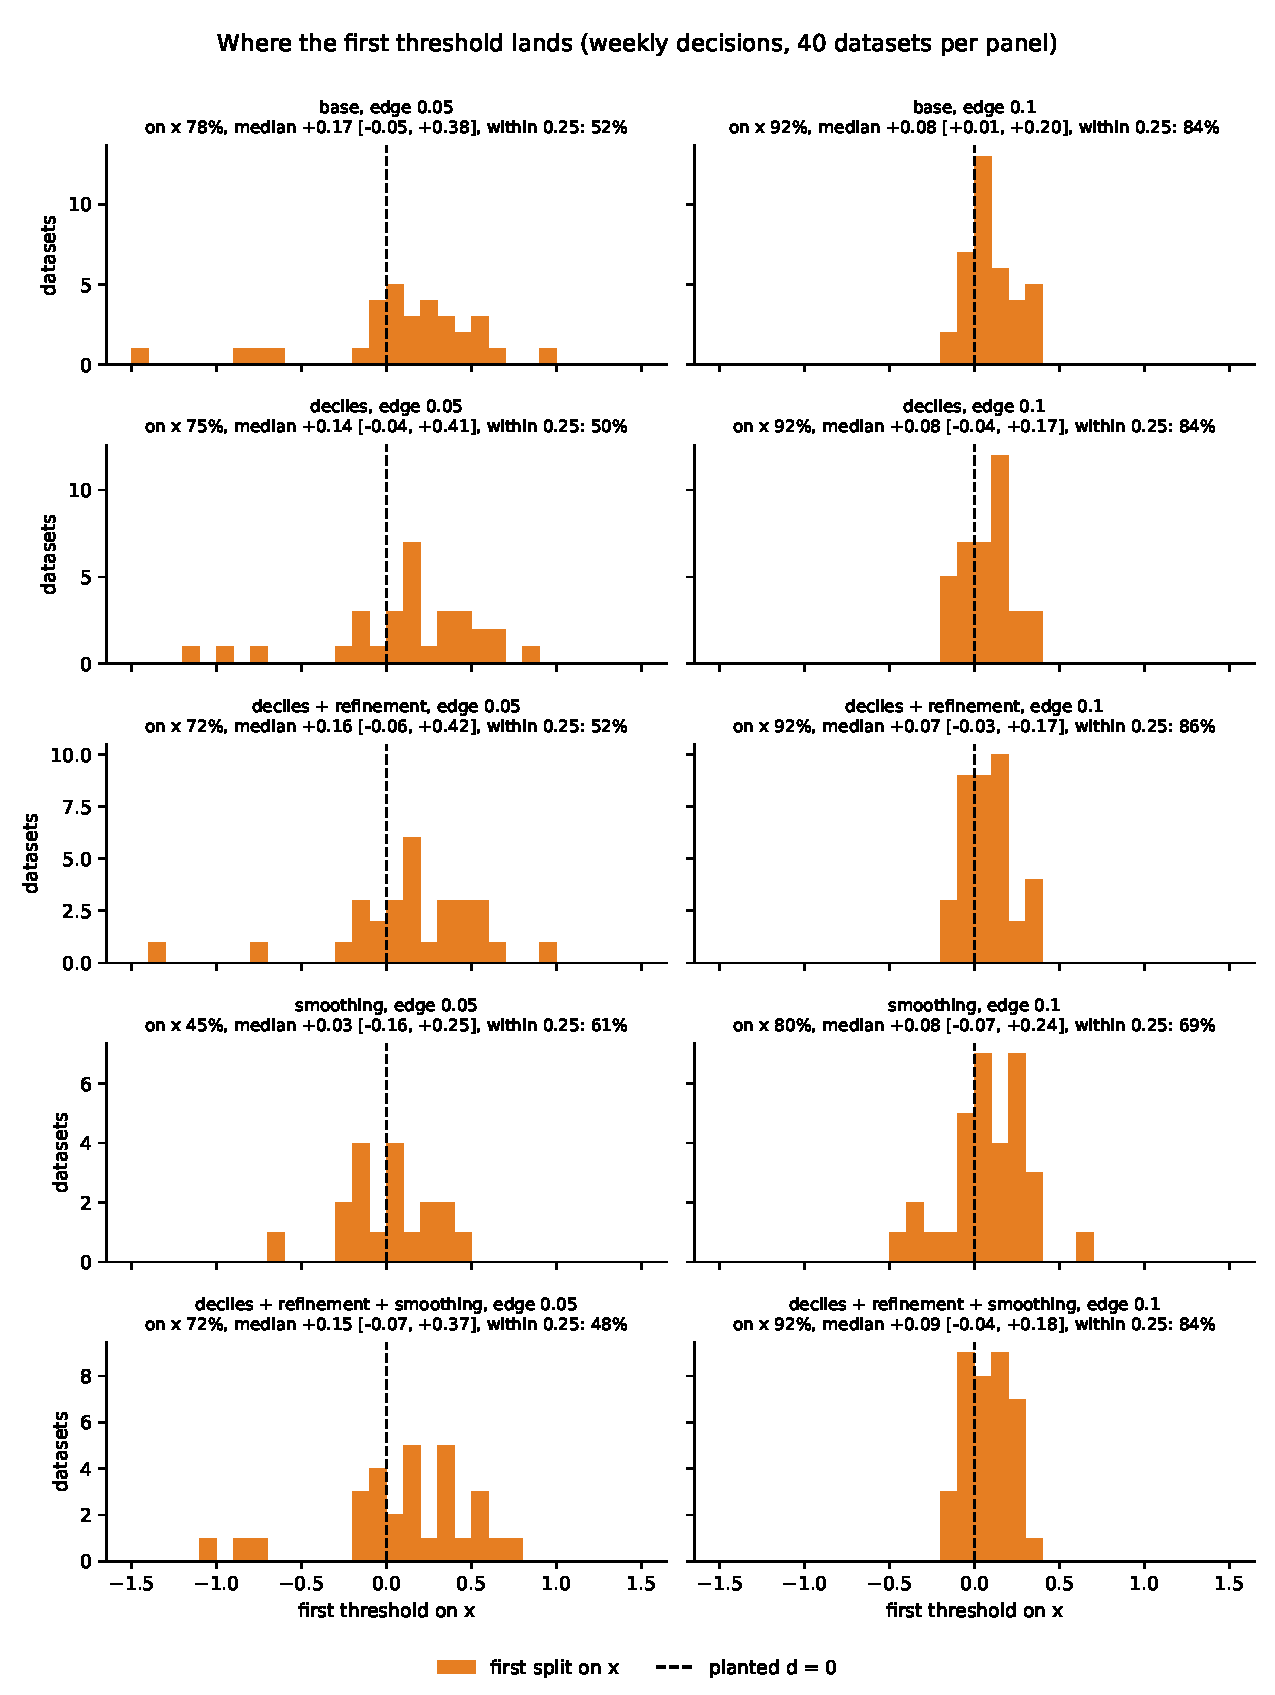
\includegraphics[width=0.9\linewidth]{split_options_thresholds}
\caption{Weekly decisions: where the first threshold lands, one row per setting; \emph{left:} edge 0.05, \emph{right:} edge 0.10. The target is $d=0$.}
\label{fig:enh-thresholds}
\end{figure}
\begin{figure}[H]
\centering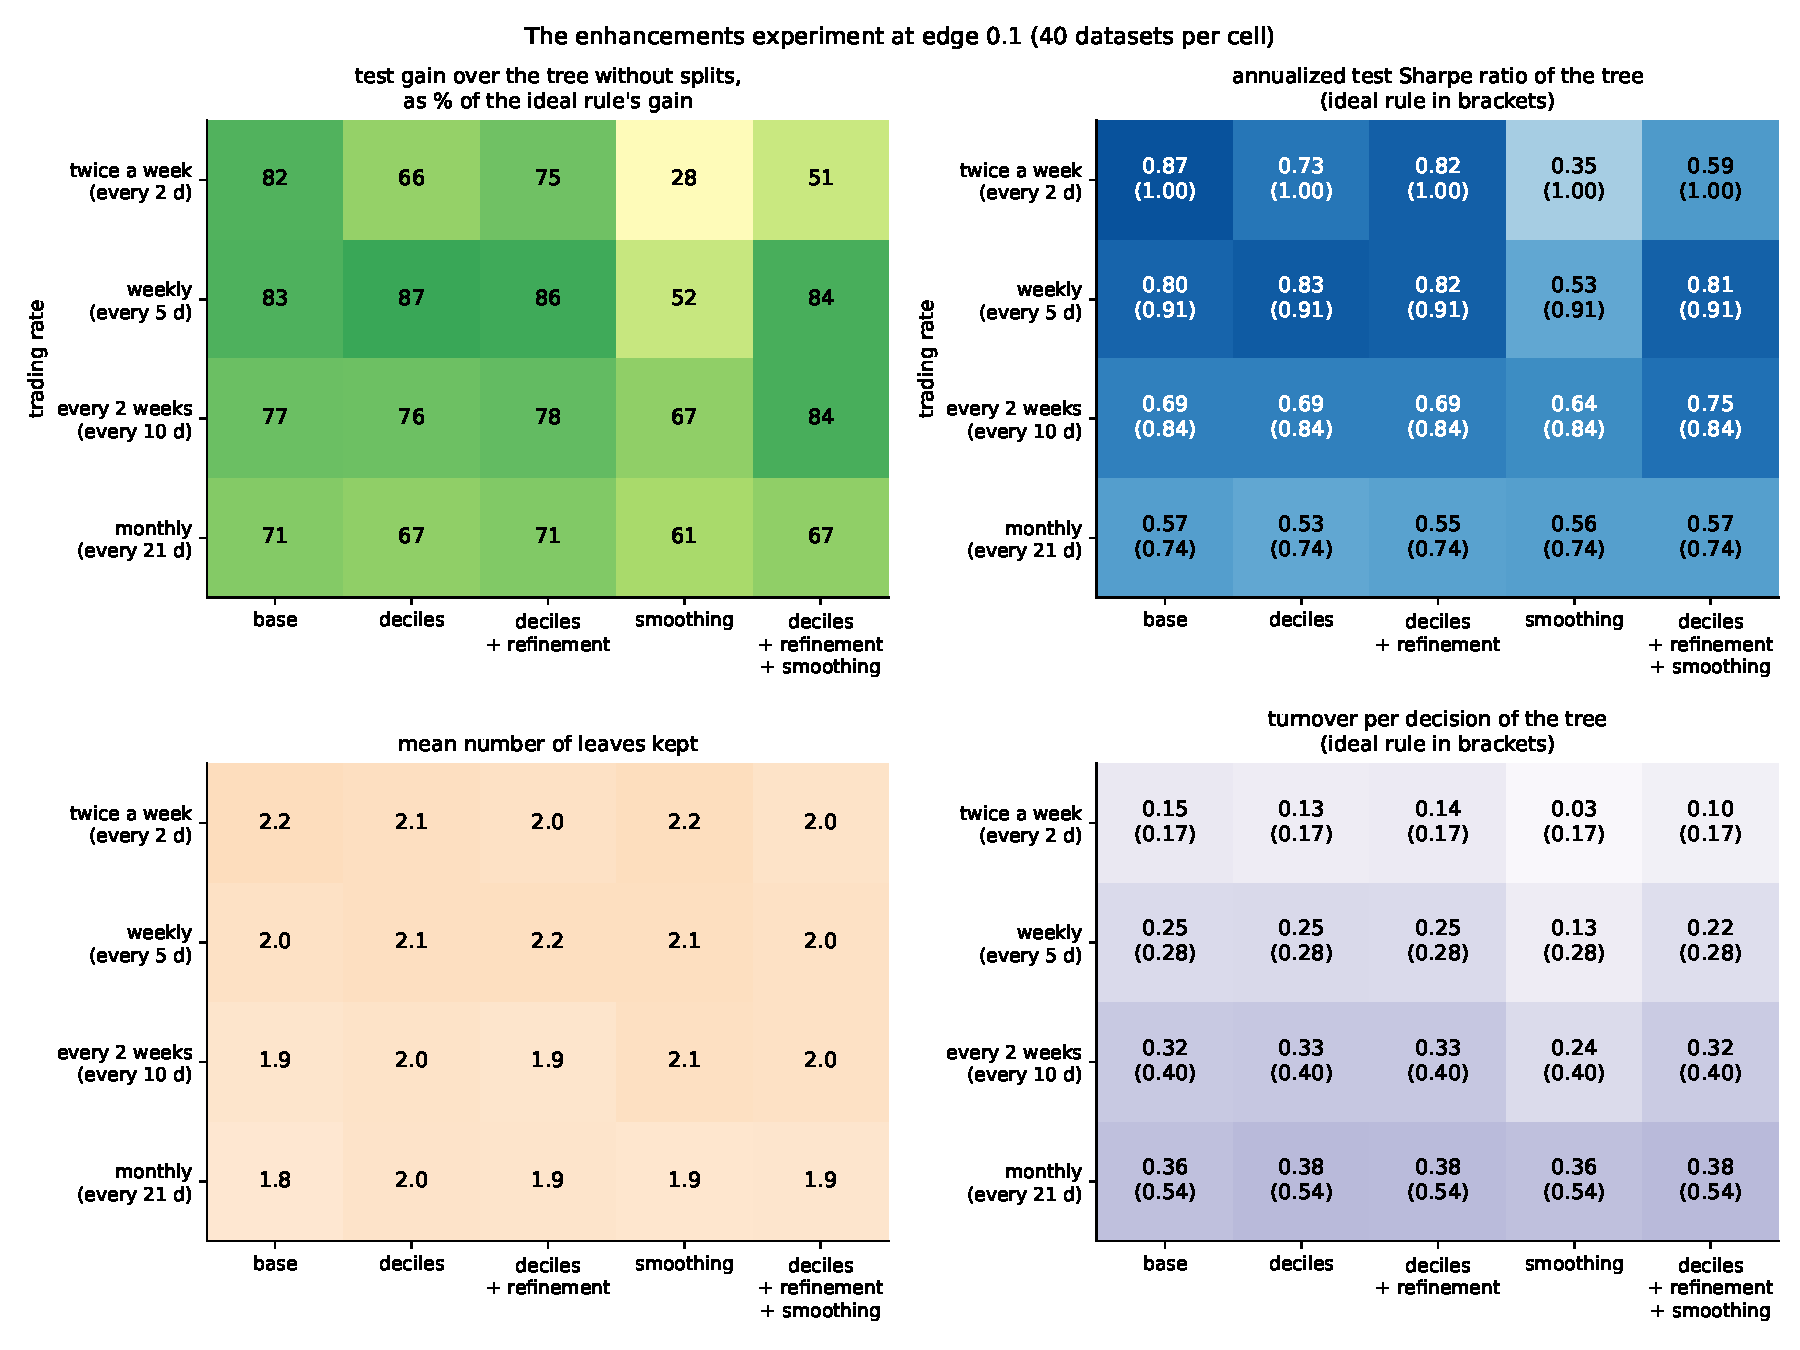
\includegraphics[width=0.95\linewidth]{split_options_maps}
\caption{Edge 0.10, rows: trading rate, columns: setting. Share of the ideal rule's test gain captured; annualized test Sharpe ratio (ideal rule in brackets); mean number of leaves; turnover per decision (ideal rule in brackets).}
\label{fig:enh-maps}
\end{figure}

\begin{table}[H]
\centering\footnotesize
\setlength{\tabcolsep}{3pt}
\begin{tabular}{@{}l r r rr r r r rr r@{}}
\toprule
& & & \multicolumn{2}{c}{splits (\%)} & \multicolumn{2}{c}{first threshold on $x$} & & \multicolumn{2}{c}{annual.\ Sharpe} & gain\\
\cmidrule(lr){4-5}\cmidrule(lr){6-7}\cmidrule(lr){9-10}
setting & $h$ & leaves & on $x$ & none & median [quartiles] & $|\cdot|\le0.25$ & spread & tree & ideal & captured\\
\midrule
base & 2 & 2.2 & 98 & 2 & $+0.03\ [-0.01,+0.12]$ & 97\% & -- & 0.87 & 1.00 & 82\%\\
 & 5 & 2.0 & 92 & 8 & $+0.08\ [+0.01,+0.20]$ & 84\% & -- & 0.80 & 0.91 & 83\%\\
 & 10 & 1.9 & 88 & 12 & $+0.05\ [-0.10,+0.26]$ & 63\% & -- & 0.69 & 0.84 & 77\%\\
 & 21 & 1.8 & 72 & 28 & $+0.09\ [-0.19,+0.29]$ & 45\% & -- & 0.57 & 0.74 & 71\%\\
\midrule
deciles & 2 & 2.1 & 95 & 5 & $+0.06\ [-0.03,+0.12]$ & 87\% & -- & 0.73 & 1.00 & 66\%\\
 & 5 & 2.1 & 92 & 8 & $+0.08\ [-0.04,+0.17]$ & 84\% & -- & 0.83 & 0.91 & 87\%\\
 & 10 & 2.0 & 88 & 12 & $+0.11\ [-0.03,+0.22]$ & 71\% & -- & 0.69 & 0.84 & 76\%\\
 & 21 & 2.0 & 75 & 25 & $+0.04\ [-0.22,+0.19]$ & 57\% & -- & 0.53 & 0.74 & 67\%\\
\midrule
deciles + refinement & 2 & 2.1 & 95 & 5 & $+0.07\ [-0.04,+0.12]$ & 87\% & -- & 0.82 & 1.00 & 75\%\\
 & 5 & 2.2 & 92 & 8 & $+0.07\ [-0.03,+0.17]$ & 86\% & -- & 0.82 & 0.91 & 86\%\\
 & 10 & 1.9 & 88 & 12 & $+0.07\ [-0.09,+0.24]$ & 71\% & -- & 0.69 & 0.84 & 78\%\\
 & 21 & 2.0 & 75 & 25 & $+0.04\ [-0.21,+0.20]$ & 57\% & -- & 0.55 & 0.74 & 71\%\\
\midrule
smoothing & 2 & 2.2 & 78 & 22 & $+0.09\ [-0.02,+0.23]$ & 74\% & 0.65 & 0.35 & 1.00 & 28\%\\
 & 5 & 2.2 & 80 & 20 & $+0.08\ [-0.07,+0.24]$ & 69\% & 0.64 & 0.53 & 0.91 & 52\%\\
 & 10 & 2.1 & 80 & 20 & $+0.07\ [-0.05,+0.23]$ & 62\% & 0.70 & 0.64 & 0.84 & 67\%\\
 & 21 & 1.9 & 75 & 25 & $+0.10\ [-0.08,+0.17]$ & 87\% & 0.68 & 0.56 & 0.74 & 61\%\\
\midrule
all three & 2 & 2.0 & 85 & 15 & $+0.05\ [+0.00,+0.12]$ & 85\% & 0.18 & 0.59 & 1.00 & 51\%\\
 & 5 & 2.1 & 92 & 8 & $+0.09\ [-0.04,+0.18]$ & 84\% & 0.18 & 0.81 & 0.91 & 84\%\\
 & 10 & 2.1 & 92 & 8 & $+0.07\ [-0.07,+0.27]$ & 68\% & 0.19 & 0.75 & 0.84 & 84\%\\
 & 21 & 1.9 & 80 & 20 & $+0.03\ [-0.16,+0.18]$ & 69\% & 0.21 & 0.57 & 0.74 & 67\%\\
\bottomrule
\end{tabular}
\caption{The split-search options at edge 0.10, 40 datasets per row ($h$: days between decisions; turnover is in Figure~\ref{fig:enh-maps}). At edge 0.05 no setting improves on the base (gain captured 36--48\% for the base, 28--56\% with deciles, with or without refinement, 13--48\% with all three), and smoothing alone loses most of it (8--23\%).}
\label{tab:enhancements}
\end{table}

\textbf{Reading the figures and the table.}
\begin{itemize}\setlength{\itemsep}{1pt}
\item \textbf{Deciles make the threshold steadier at the slow rates}: the share within $0.25$ of $d$ rises from 63 to 71\% every two weeks and from 45 to 57\% monthly, and the quartile width falls from 0.36 to 0.25 and from 0.48 to 0.41. Weekly and every two weeks the Sharpe ratio is unchanged; at the fastest rate the coarse grid costs 0.14 of Sharpe (0.73 against 0.87), because there the data can pin the threshold finer than a decile.
\item \textbf{The refinement removes most of that cost} (0.82 at every 2 days, 75\% of the gain against 66\%) and keeps the steadier thresholds. Deciles with refinement match the base within noise everywhere (Sharpe 0.82, 0.82, 0.69, 0.55 against 0.87, 0.80, 0.69, 0.57) and centre the threshold better at the slow rates: a reasonable default for slow trading.
\item \textbf{Smoothing alone, at $\kappa=1$, is too wide and it interacts badly with the fee.} The weights spread over about $\pm0.3$ (spread 0.65): near $d$ the expected return is small, so thresholds within that band are within one standard error of each other. The score then rises gradually from about zero (Figure~\ref{fig:scores}) and, with $\lambda=1$, stays inside the no-trade window of the optimizer for most decisions: the tree trades three to five times less (turnover 0.03 against 0.15 at every 2 days) and captures 28 to 67\% of the gain instead of 77 to 83\%. Smoothing the \emph{score} is not sizing the \emph{position}: with a proportional fee a small score means ``do not trade'', not ``trade a little''.
\item \textbf{All three together}: the candidate set (the deciles and the refinement window) confines the weights, spread 0.18 to 0.21, and the threshold is as steady as with deciles (85, 84, 68 and 69\% within $0.25$). Every two weeks this setting captures the most of all (84\%) with the best Sharpe ratio (0.75 against 0.69), monthly it matches the base (0.57), and at every 2 days it still pays for the soft edge (51\% of the gain, Sharpe 0.59).
\item \textbf{Next steps.} A sharper weight ($\kappa\approx0.3$, or $e^{-z^2/2\kappa^2}$) should keep the soft edge where the data are undecided without pushing the score into the no-trade window; and smoothing is worth more where positions are meant to be interior, that is with $\lambda\ge5$ (Section~\ref{sec:settings}) or a quadratic cost. Deciles with refinement can be switched on now for slow trading rates. The spurious second-level splits (10 to 25\% of the datasets keep one, Table~\ref{tab:enhancements} counts them in the leaves) are the object of Section~\ref{sec:pruning}.
\end{itemize}


\section{A fourth experiment: a calibrated pruning hurdle}\label{sec:pruning}
\textbf{Pipeline used.} P3b with \code{prune_standard_errors} set to 1 or 2, alone and on top of deciles with refinement.

\textbf{Why.} Pruning keeps a split if, on the checking decisions, it lowers the mean regret by more than $10^{-6}$ and raises the Sharpe ratio by more than 0. Those hurdles are effectively zero, so a split confirmed by a handful of noisy decisions passes; that is how the spurious second-level leaves of Sections~\ref{sec:results} and~\ref{sec:enhancements} survive. A new option, \code{prune_standard_errors}${}=k_p$, keeps a split only if its checking-row gain $\bar g$ (mean over the checking decisions of the regret without the split minus the regret with it) exceeds $k_p$ standard errors of that mean, a paired test (\code{model_and_training_pipeline.tex}, Section~9, step~5). It was run with $k_p=1$ and $k_p=2$, alone and on top of deciles with refinement, in the world and protocol of Section~\ref{sec:settings} (rates 2, 5, 10 and 21 days, edges 0.05 and 0.10, 40 datasets per cell, $\lambda=1$).

\begin{figure}[H]
\centering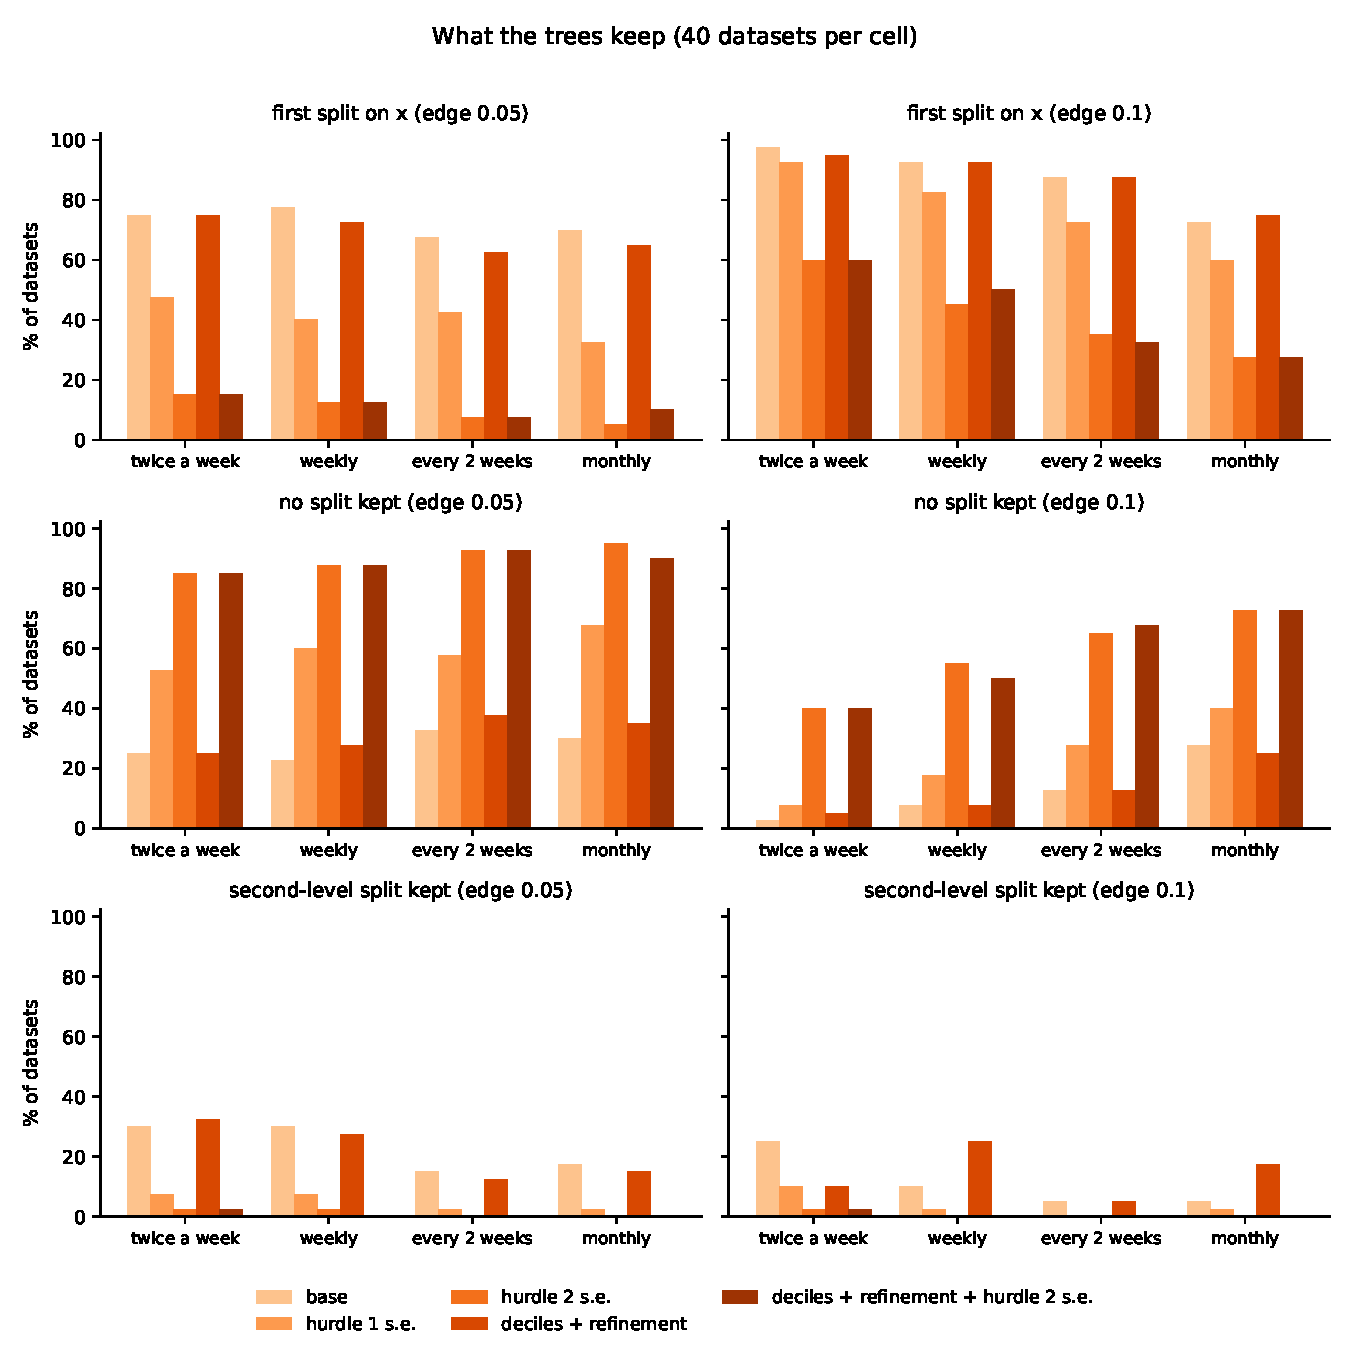
\includegraphics[width=0.9\linewidth]{pruning_hurdle_splits}
\caption{What the trees keep, by setting and trading rate: first split on $x$, no split kept, a second-level split kept (\% of the datasets). \emph{Top:} edge 0.05; \emph{bottom:} edge 0.10.}
\label{fig:pruning-splits}
\end{figure}
\begin{figure}[H]
\centering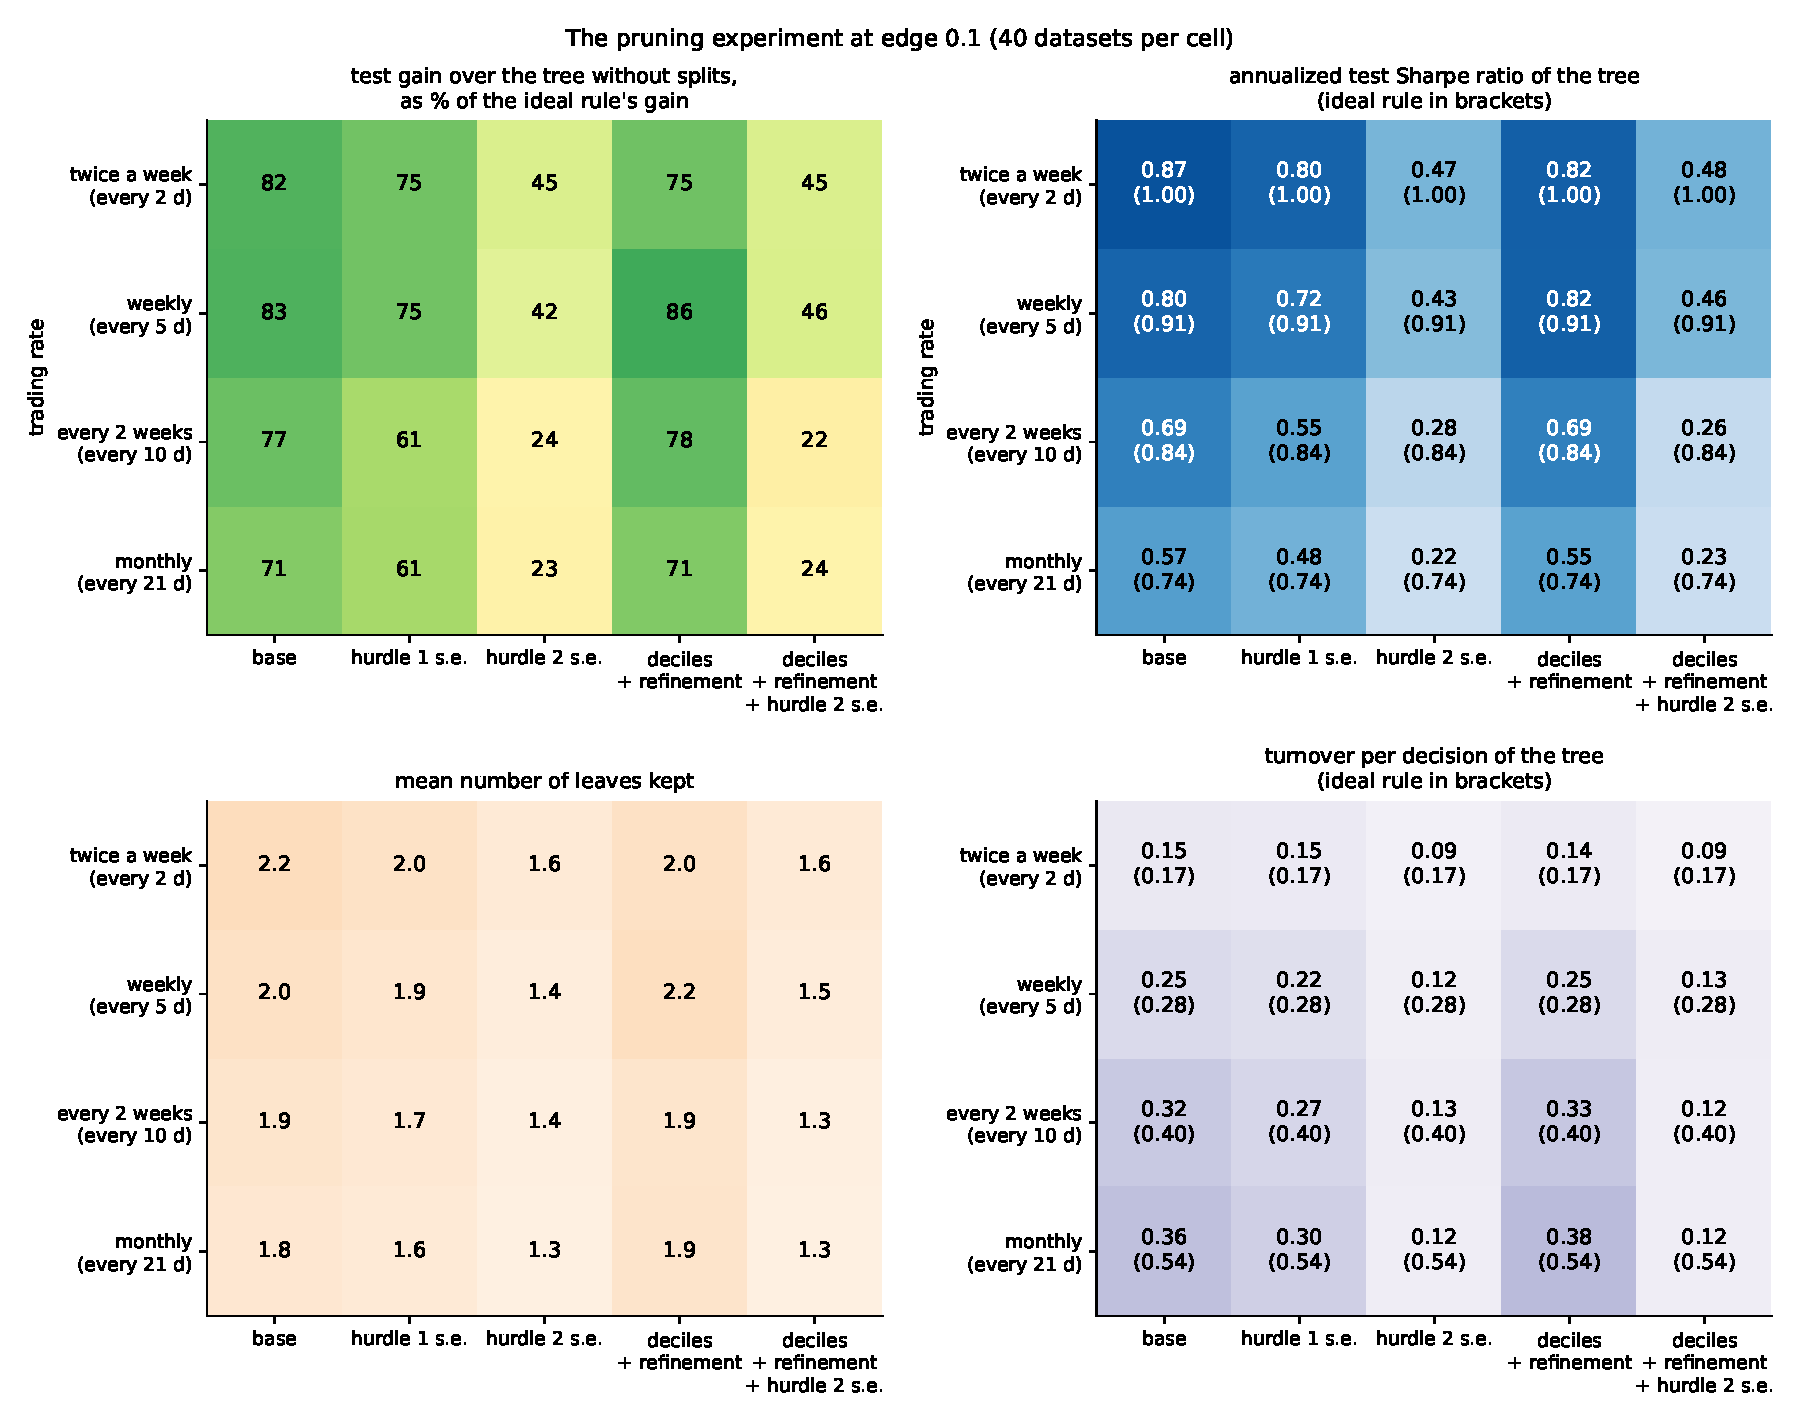
\includegraphics[width=0.95\linewidth]{pruning_hurdle_maps}
\caption{Edge 0.10, rows: trading rate, columns: setting. Share of the ideal rule's test gain captured; annualized test Sharpe ratio (ideal rule in brackets); mean number of leaves; turnover per decision (ideal rule in brackets).}
\label{fig:pruning-maps}
\end{figure}
\begin{figure}[H]
\centering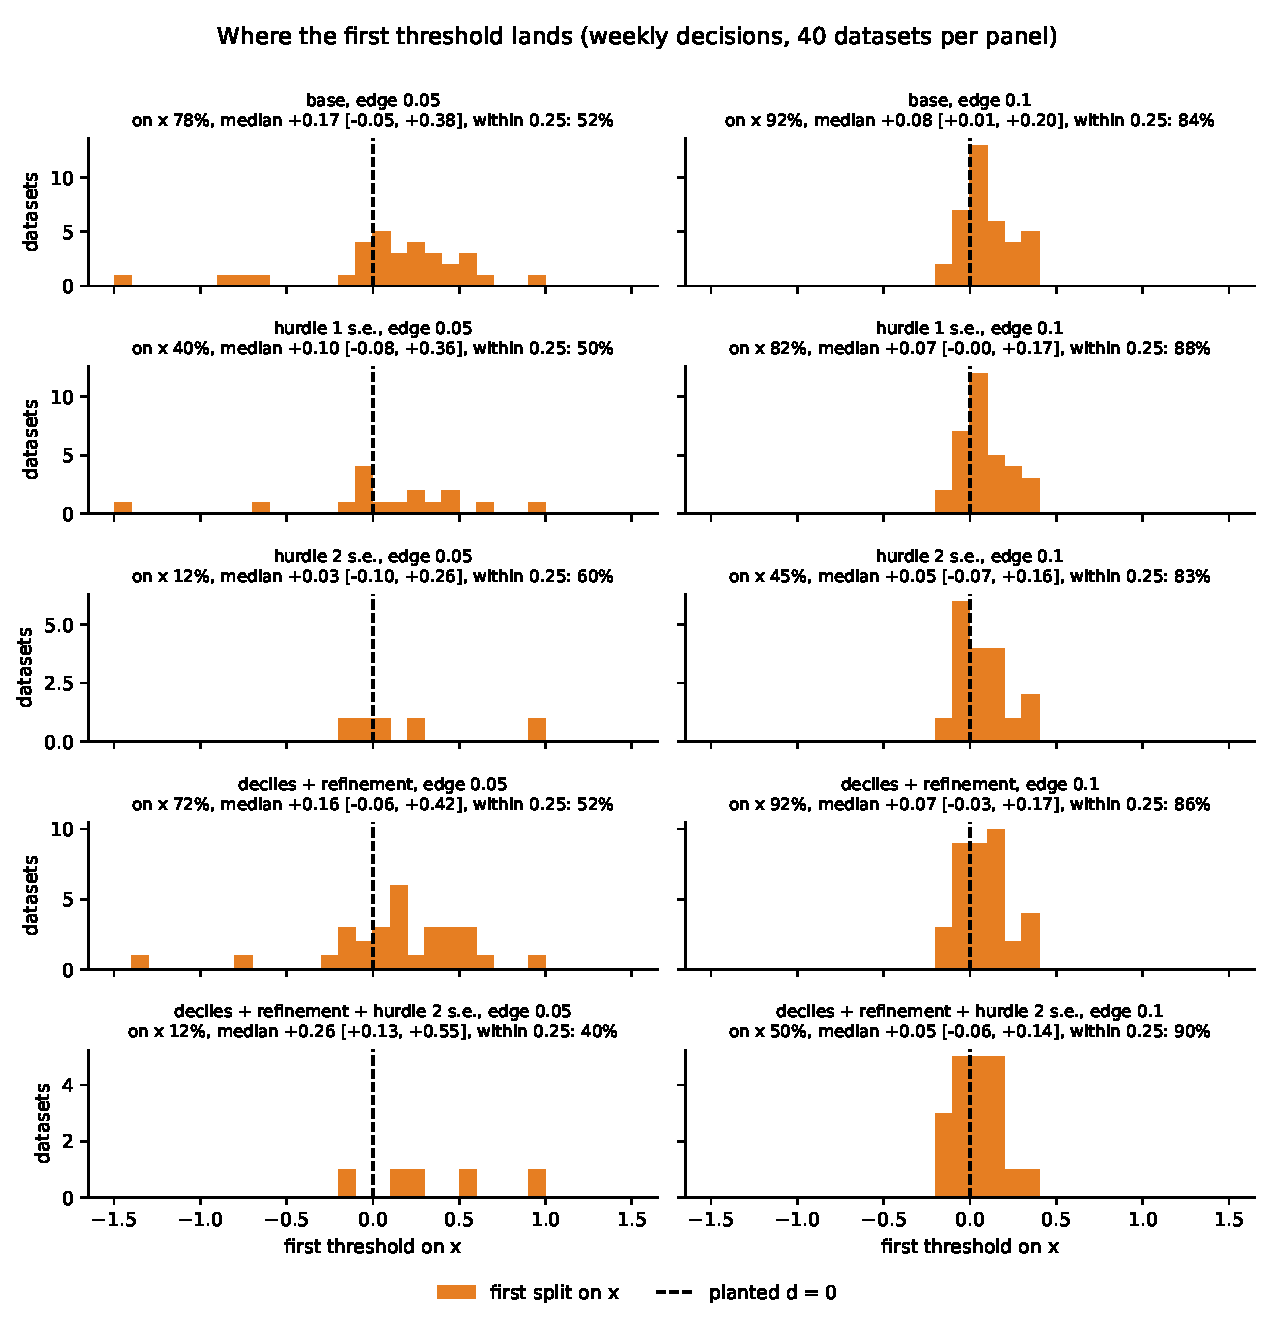
\includegraphics[width=0.9\linewidth]{pruning_hurdle_thresholds}
\caption{Weekly decisions: where the first threshold lands, one row per setting; \emph{left:} edge 0.05, \emph{right:} edge 0.10.}
\label{fig:pruning-thresholds}
\end{figure}

\begin{table}[H]
\centering\small
\setlength{\tabcolsep}{4pt}
\begin{tabular}{@{}l r rrr r rr r@{}}
\toprule
& & \multicolumn{3}{c}{datasets (\%)} & threshold & \multicolumn{2}{c}{annual.\ Sharpe} & gain\\
\cmidrule(lr){3-5}\cmidrule(lr){7-8}
setting & $h$ & on $x$ & none & 2nd level & $|\cdot|\le0.25$ & tree & ideal & captured\\
\midrule
base & 2 & 98 & 2 & 25 & 97\% & 0.87 & 1.00 & 82\%\\
 & 5 & 92 & 8 & 10 & 84\% & 0.80 & 0.91 & 83\%\\
 & 10 & 88 & 12 & 5 & 63\% & 0.69 & 0.84 & 77\%\\
 & 21 & 72 & 28 & 5 & 45\% & 0.57 & 0.74 & 71\%\\
\midrule
hurdle 1 s.e. & 2 & 92 & 8 & 10 & 100\% & 0.80 & 1.00 & 75\%\\
 & 5 & 82 & 18 & 2 & 88\% & 0.72 & 0.91 & 75\%\\
 & 10 & 72 & 28 & 0 & 66\% & 0.55 & 0.84 & 61\%\\
 & 21 & 60 & 40 & 2 & 50\% & 0.48 & 0.74 & 61\%\\
\midrule
hurdle 2 s.e. & 2 & 60 & 40 & 2 & 100\% & 0.47 & 1.00 & 45\%\\
 & 5 & 45 & 55 & 0 & 83\% & 0.43 & 0.91 & 42\%\\
 & 10 & 35 & 65 & 0 & 43\% & 0.28 & 0.84 & 24\%\\
 & 21 & 28 & 72 & 0 & 55\% & 0.22 & 0.74 & 23\%\\
\midrule
deciles + refinement & 2 & 95 & 5 & 10 & 87\% & 0.82 & 1.00 & 75\%\\
 & 5 & 92 & 8 & 25 & 86\% & 0.82 & 0.91 & 86\%\\
 & 10 & 88 & 12 & 5 & 71\% & 0.69 & 0.84 & 78\%\\
 & 21 & 75 & 25 & 18 & 57\% & 0.55 & 0.74 & 71\%\\
\midrule
deciles + refinement + hurdle 2 s.e. & 2 & 60 & 40 & 2 & 92\% & 0.48 & 1.00 & 45\%\\
 & 5 & 50 & 50 & 0 & 90\% & 0.46 & 0.91 & 46\%\\
 & 10 & 32 & 68 & 0 & 62\% & 0.26 & 0.84 & 22\%\\
 & 21 & 28 & 72 & 0 & 45\% & 0.23 & 0.74 & 24\%\\
\bottomrule
\end{tabular}
\caption{The pruning hurdle at edge 0.10, 40 datasets per row ($h$: days between decisions; ``2nd level'': datasets that keep a second-level split). At edge 0.05 the hurdle of 1 s.e.\ halves the trees that split (32--48\% against 68--78\%) and their Sharpe ratio (0.10--0.15 against 0.19--0.27); at 2 s.e.\ almost nothing survives (5--15\% split, Sharpe about 0.05).}
\label{tab:pruning}
\end{table}

\textbf{Reading the figures and the table.}
\begin{itemize}\setlength{\itemsep}{1pt}
\item \textbf{The hurdle does remove the spurious leaves}: at 1 s.e.\ the second-level splits fall from 25, 10, 5 and 5\% of the datasets to 10, 2, 0 and 2\%, and at 2 s.e.\ to 2, 0, 0 and 0\%; the thresholds that survive are the best-centred of all the experiments (100 and 88\% within $0.25$ at every 2 days and weekly).
\item \textbf{But it removes true splits faster than it earns.} At 1 s.e.\ the first split on $x$ falls from 98, 92, 88 and 72\% to 92, 82, 72 and 60\%, and the Sharpe ratio by 0.07 to 0.14; at 2 s.e.\ about half of the root splits are gone (45\% at weekly decisions) and the Sharpe ratio halves. The tree without splits is a poor fallback here: it holds cash or drifts, so every true split lost costs the whole edge.
\item \textbf{Why the test has so little power.} The checking block is a quarter of the training rows, 189 decisions at weekly trading. For dataset 42 the root split's gain there is $0.0031\pm0.0011$ per decision ($z=2.8$) and the tail leaf's $0.00014\pm0.0003$ ($z=0.5$): a true split at edge 0.10 typically clears one standard error and often not two, while the noise leaves sit below one. A hurdle that separates them needs more checking decisions than a 25\% block provides, and at edge 0.05 no hurdle can separate them at all.
\item \textbf{Deciles with refinement change nothing on this point}: the same hurdle gives the same losses on top of them.
\item \textbf{What to do instead.} The spurious leaves are second-level splits, while the root split is confirmed 92 to 98\% of the time at edge 0.10 without any hurdle. A hurdle applied only below the root (a depth-dependent $k_p$) would remove the noise leaves at no cost to the root split; a larger checking block (40\% instead of 25\%) would raise the power of the test at the cost of growth data. Both are cheap to test. Until then, $k_p=0$ stays the default, and the spurious leaves are better limited by the minimum leaf fraction of Section~\ref{sec:enhancements}.
\end{itemize}


\section{A fifth experiment: the resolution of the threshold against noise}\label{sec:resolution}
\textbf{Pipeline used.} P3b with every option off, identical to P2; market M2 with observation noise on the feature (M2').

\textbf{Why.} Sections~\ref{sec:results} to~\ref{sec:pruning} fixed the noise: a volatility of 1\% a day and a feature observed exactly. Two questions remain about what the tree can resolve. How far can the price volatility rise, at a fixed drift, before the two regimes can no longer be told apart? And how much observation noise on the feature can the threshold survive? The second is not a question about the variance of $x$: the tree only sees the ordering of $x$, so scaling $x$ changes nothing; what blurs a feature is noise \emph{added} to it, $x^{\mathrm{obs}}_t=x_t+\tau\varepsilon_t$ with $\varepsilon_t$ white, the price still following the true $x_t$. Two sweeps, at weekly and monthly decisions, 60 datasets per point:
\begin{itemize}\setlength{\itemsep}{1pt}
\item the price volatility from 0.4\% to 4\% a day at a fixed regime drift of $\pm25\%$ a year, so the edge $e=\mu/\sigma$ runs from 0.25 down to 0.025;
\item the observation noise $\tau$ from 0 to 2 standard deviations of $x$, at the base volatility.
\end{itemize}
With a noisy feature the tree sees $x^{\mathrm{obs}}$, and so does the ideal rule: it is fed with the expected return given the \emph{observed} value, $\E[g_h(x)\mid x^{\mathrm{obs}}]$, computed by drawing the true $x$ from its Gaussian posterior (the true value shrinks towards the mean by $s^2/(s^2+\tau^2)$). The threshold to find stays $d=0$ by symmetry.

\begin{figure}[H]
\centering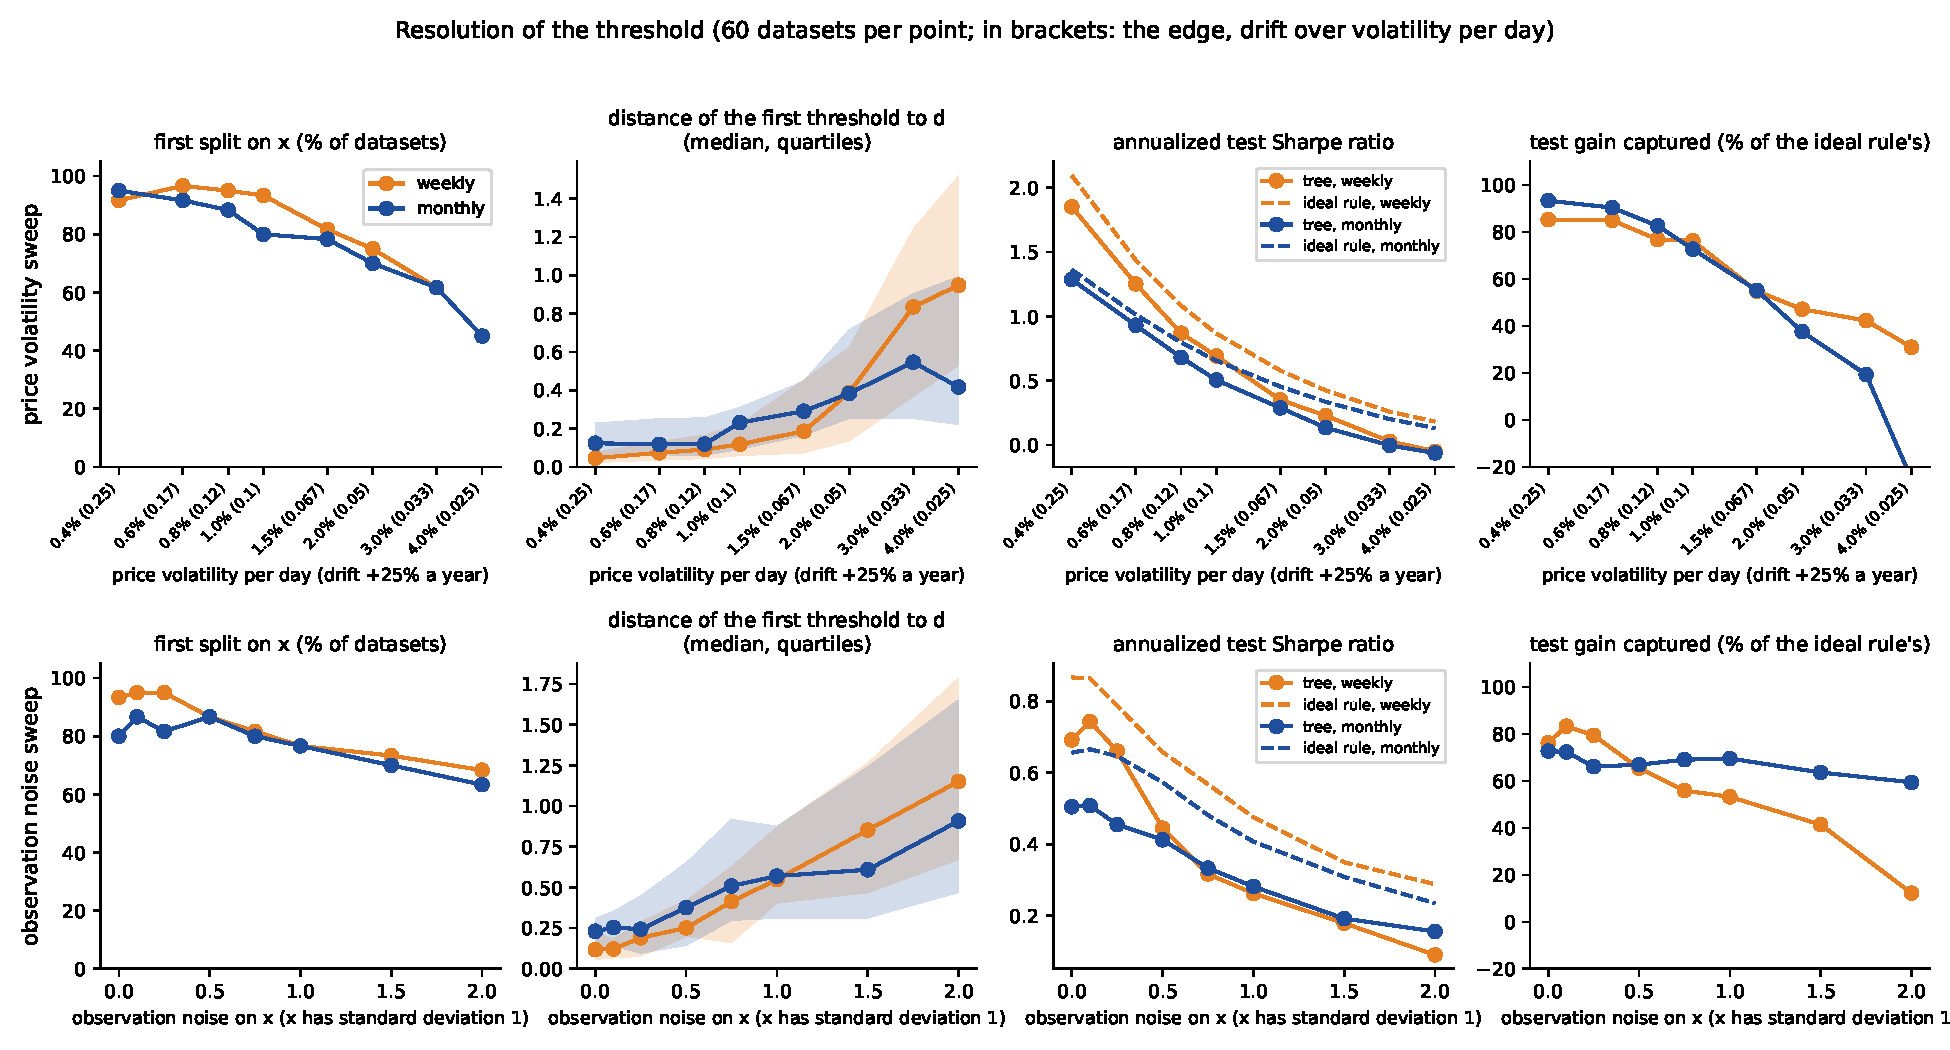
\includegraphics[width=\linewidth]{resolution_curves}
\caption{\emph{Top:} the price volatility sweep (the edge in brackets); \emph{bottom:} the observation-noise sweep. From left to right: datasets whose first split is on $x$; distance of the first threshold to $d$ (median and quartiles over the datasets that split); annualized test Sharpe ratio of the tree (solid) and of the ideal rule (dashed); share of the ideal rule's gain captured. Orange: weekly decisions; blue: monthly.}
\label{fig:resolution}
\end{figure}

\begin{table}[H]
\centering\footnotesize
\setlength{\tabcolsep}{3.5pt}
\begin{tabular}{@{}l r r rr r rr r@{}}
\toprule
& & & \multicolumn{2}{c}{splits (\%)} & first threshold & \multicolumn{2}{c}{annual.\ Sharpe} & gain\\
\cmidrule(lr){4-5}\cmidrule(lr){7-8}
sweep & value & edge & on $x$ & none & $|\theta|$: median [quartiles] & tree & ideal & captured\\
\midrule
volatility, weekly & 0.4\% & 0.25 & 92 & 8 & $0.05\ [0.02, 0.08]$ & 1.85 & 2.10 & 85\%\\
 & 0.6\% & 0.17 & 97 & 3 & $0.07\ [0.03, 0.13]$ & 1.25 & 1.44 & 85\%\\
 & 0.8\% & 0.125 & 95 & 5 & $0.09\ [0.04, 0.17]$ & 0.87 & 1.08 & 77\%\\
 & 1.0\% & 0.10 & 93 & 7 & $0.12\ [0.06, 0.22]$ & 0.69 & 0.87 & 76\%\\
 & 1.5\% & 0.067 & 82 & 18 & $0.19\ [0.07, 0.45]$ & 0.35 & 0.58 & 55\%\\
 & 2.0\% & 0.05 & 75 & 25 & $0.39\ [0.14, 0.62]$ & 0.23 & 0.42 & 47\%\\
 & 3.0\% & 0.033 & 62 & 38 & $0.83\ [0.37, 1.24]$ & 0.03 & 0.26 & 42\%\\
 & 4.0\% & 0.025 & 45 & 55 & $0.95\ [0.53, 1.52]$ & $-0.05$ & 0.18 & 31\%\\
\midrule
volatility, monthly & 0.4\% & 0.25 & 95 & 5 & $0.12\ [0.06, 0.23]$ & 1.29 & 1.36 & 93\%\\
 & 0.6\% & 0.17 & 92 & 8 & $0.12\ [0.06, 0.25]$ & 0.93 & 1.01 & 90\%\\
 & 0.8\% & 0.125 & 88 & 12 & $0.12\ [0.06, 0.26]$ & 0.68 & 0.80 & 83\%\\
 & 1.0\% & 0.10 & 80 & 20 & $0.23\ [0.09, 0.31]$ & 0.51 & 0.66 & 73\%\\
 & 1.5\% & 0.067 & 78 & 22 & $0.29\ [0.16, 0.45]$ & 0.29 & 0.45 & 55\%\\
 & 2.0\% & 0.05 & 70 & 30 & $0.38\ [0.25, 0.72]$ & 0.13 & 0.33 & 38\%\\
 & 3.0\% & 0.033 & 62 & 38 & $0.55\ [0.25, 0.90]$ & 0.00 & 0.20 & 19\%\\
 & 4.0\% & 0.025 & 45 & 55 & $0.42\ [0.22, 0.99]$ & $-0.06$ & 0.13 & $-25$\%\\
\midrule
noise $\tau$, weekly & 0 & 0.10 & 93 & 7 & $0.12\ [0.06, 0.22]$ & 0.69 & 0.87 & 76\%\\
 & 0.1 & 0.10 & 95 & 5 & $0.12\ [0.07, 0.18]$ & 0.74 & 0.86 & 83\%\\
 & 0.25 & 0.10 & 95 & 5 & $0.19\ [0.08, 0.29]$ & 0.66 & 0.79 & 79\%\\
 & 0.5 & 0.10 & 87 & 13 & $0.25\ [0.20, 0.42]$ & 0.45 & 0.66 & 65\%\\
 & 0.75 & 0.10 & 82 & 18 & $0.41\ [0.16, 0.63]$ & 0.32 & 0.57 & 56\%\\
 & 1 & 0.10 & 77 & 23 & $0.55\ [0.40, 0.87]$ & 0.26 & 0.48 & 53\%\\
 & 1.5 & 0.10 & 73 & 27 & $0.85\ [0.47, 1.27]$ & 0.18 & 0.35 & 41\%\\
 & 2 & 0.10 & 68 & 32 & $1.15\ [0.67, 1.79]$ & 0.09 & 0.29 & 12\%\\
\midrule
noise $\tau$, monthly & 0 & 0.10 & 80 & 20 & $0.23\ [0.09, 0.31]$ & 0.51 & 0.66 & 73\%\\
 & 0.1 & 0.10 & 87 & 13 & $0.25\ [0.14, 0.35]$ & 0.51 & 0.67 & 72\%\\
 & 0.25 & 0.10 & 82 & 18 & $0.24\ [0.10, 0.45]$ & 0.45 & 0.65 & 66\%\\
 & 0.5 & 0.10 & 87 & 13 & $0.38\ [0.14, 0.65]$ & 0.41 & 0.57 & 67\%\\
 & 0.75 & 0.10 & 80 & 20 & $0.51\ [0.30, 0.92]$ & 0.33 & 0.48 & 69\%\\
 & 1 & 0.10 & 77 & 23 & $0.57\ [0.31, 0.88]$ & 0.28 & 0.41 & 70\%\\
 & 1.5 & 0.10 & 70 & 30 & $0.61\ [0.31, 1.24]$ & 0.19 & 0.31 & 64\%\\
 & 2 & 0.10 & 63 & 37 & $0.91\ [0.47, 1.65]$ & 0.16 & 0.24 & 59\%\\
\bottomrule
\end{tabular}
\caption{The resolution sweeps, 60 datasets per row. The volatility sweep keeps the drift at $\pm25\%$ a year, so the edge $e=\mu/\sigma$ falls as the volatility rises; the noise sweep keeps the base volatility and adds white noise of standard deviation $\tau$ to the observed feature ($x$ has standard deviation 1). ``Ideal'' is the optimizer fed with the expected return given the observed feature; its own Sharpe ratio falls with the noise because the observed feature carries less information.}
\label{tab:resolution}
\end{table}

\textbf{Reading the figure and the table.}
\begin{itemize}\setlength{\itemsep}{1pt}
\item \textbf{The threshold error grows like one over the edge, then breaks.} At weekly decisions the median distance to $d$ is 0.05, 0.09, 0.12 and 0.19 standard deviations of $x$ for edges 0.25, 0.125, 0.10 and 0.067 (about $0.012/e$), then 0.39 at 0.05 and 0.83 at 0.033: below an edge of about 0.05 the split is no longer located, it is guessed. The share of datasets that split follows the same break (93\% at 0.10, 75\% at 0.05, 45\% at 0.025), and so does the gain captured (76\%, 47\%, 31\%).
\item \textbf{Monthly decisions resolve less} (0.12 to 0.23 at the same edges, and 45\% found at the largest volatility as well) but capture a comparable share of a smaller ideal gain; at a volatility of 4\% a day the monthly tree earns less than no split at all.
\item \textbf{Observation noise acts like a smaller edge.} Noise of $\tau$ standard deviations shrinks the information in the observed feature by $1/(1+\tau^2)$, and the curves agree with that: $\tau=1$ at edge 0.10 gives 77\% found, an error of 0.55 and 53\% of the gain, the same picture as an edge of 0.05 without noise (75\%, 0.39, 47\%). Up to $\tau=0.25$ nothing is lost (error 0.19, 79\% of the gain); at $\tau=0.5$ the error doubles and the captured share falls to 65\%; at $\tau=2$ the tree keeps 12\% of what is left.
\item \textbf{The ideal rule degrades too}: with a noisy feature the best possible Sharpe ratio falls from 0.87 to 0.29 at $\tau=2$. The tree's loss relative to it (0.18 to 0.20 of Sharpe at every noise level up to $\tau=1$) is roughly constant: noise removes information from everybody, and the tree's own estimation error stays what it was.
\item \textbf{Practical reading.} For a regime feature to be worth a weekly tree, the drift-to-volatility ratio per day should be at least about 0.07 (a regime drift of $\pm17\%$ a year at 1\% daily volatility) and the feature should be observed with noise below a quarter of its own spread; a feature twice as noisy as that halves the attainable gain before the tree even starts.
\end{itemize}


\section{A sixth experiment: sharper smoothing weights and the hurdle below the root}\label{sec:options2}
\textbf{Pipeline used.} P4 of \code{model_history.md}: P3b plus two options, the Gaussian form of the soft-split weights (\code{smoothing_kernel}) and a pruning hurdle restricted to splits at or below a given depth (\code{prune_hurdle_from_depth}); market M2.

\textbf{Why.} Section~\ref{sec:enhancements} found the soft splits too wide at $\kappa=1$ (a spread of 0.65 standard deviations, and scores pushed into the optimizer's no-trade band), and Section~\ref{sec:pruning} found the pruning hurdle removing the true root splits along with the spurious second-level leaves. Two remedies are tested here, each alone and on top of deciles with refinement: sharper weights, $\kappa=0.5$ and $0.25$ with the Laplace form and $\kappa=1$ with the Gaussian form; and the hurdle of 2 standard errors applied only below the root, where the noise leaves live, the root split being judged by the plain rule. Same world and protocol as Section~\ref{sec:settings} (rates 2, 5, 10 and 21 days, edges 0.05 and 0.10, 40 datasets per cell, $\lambda=1$).

\begin{figure}[H]
\centering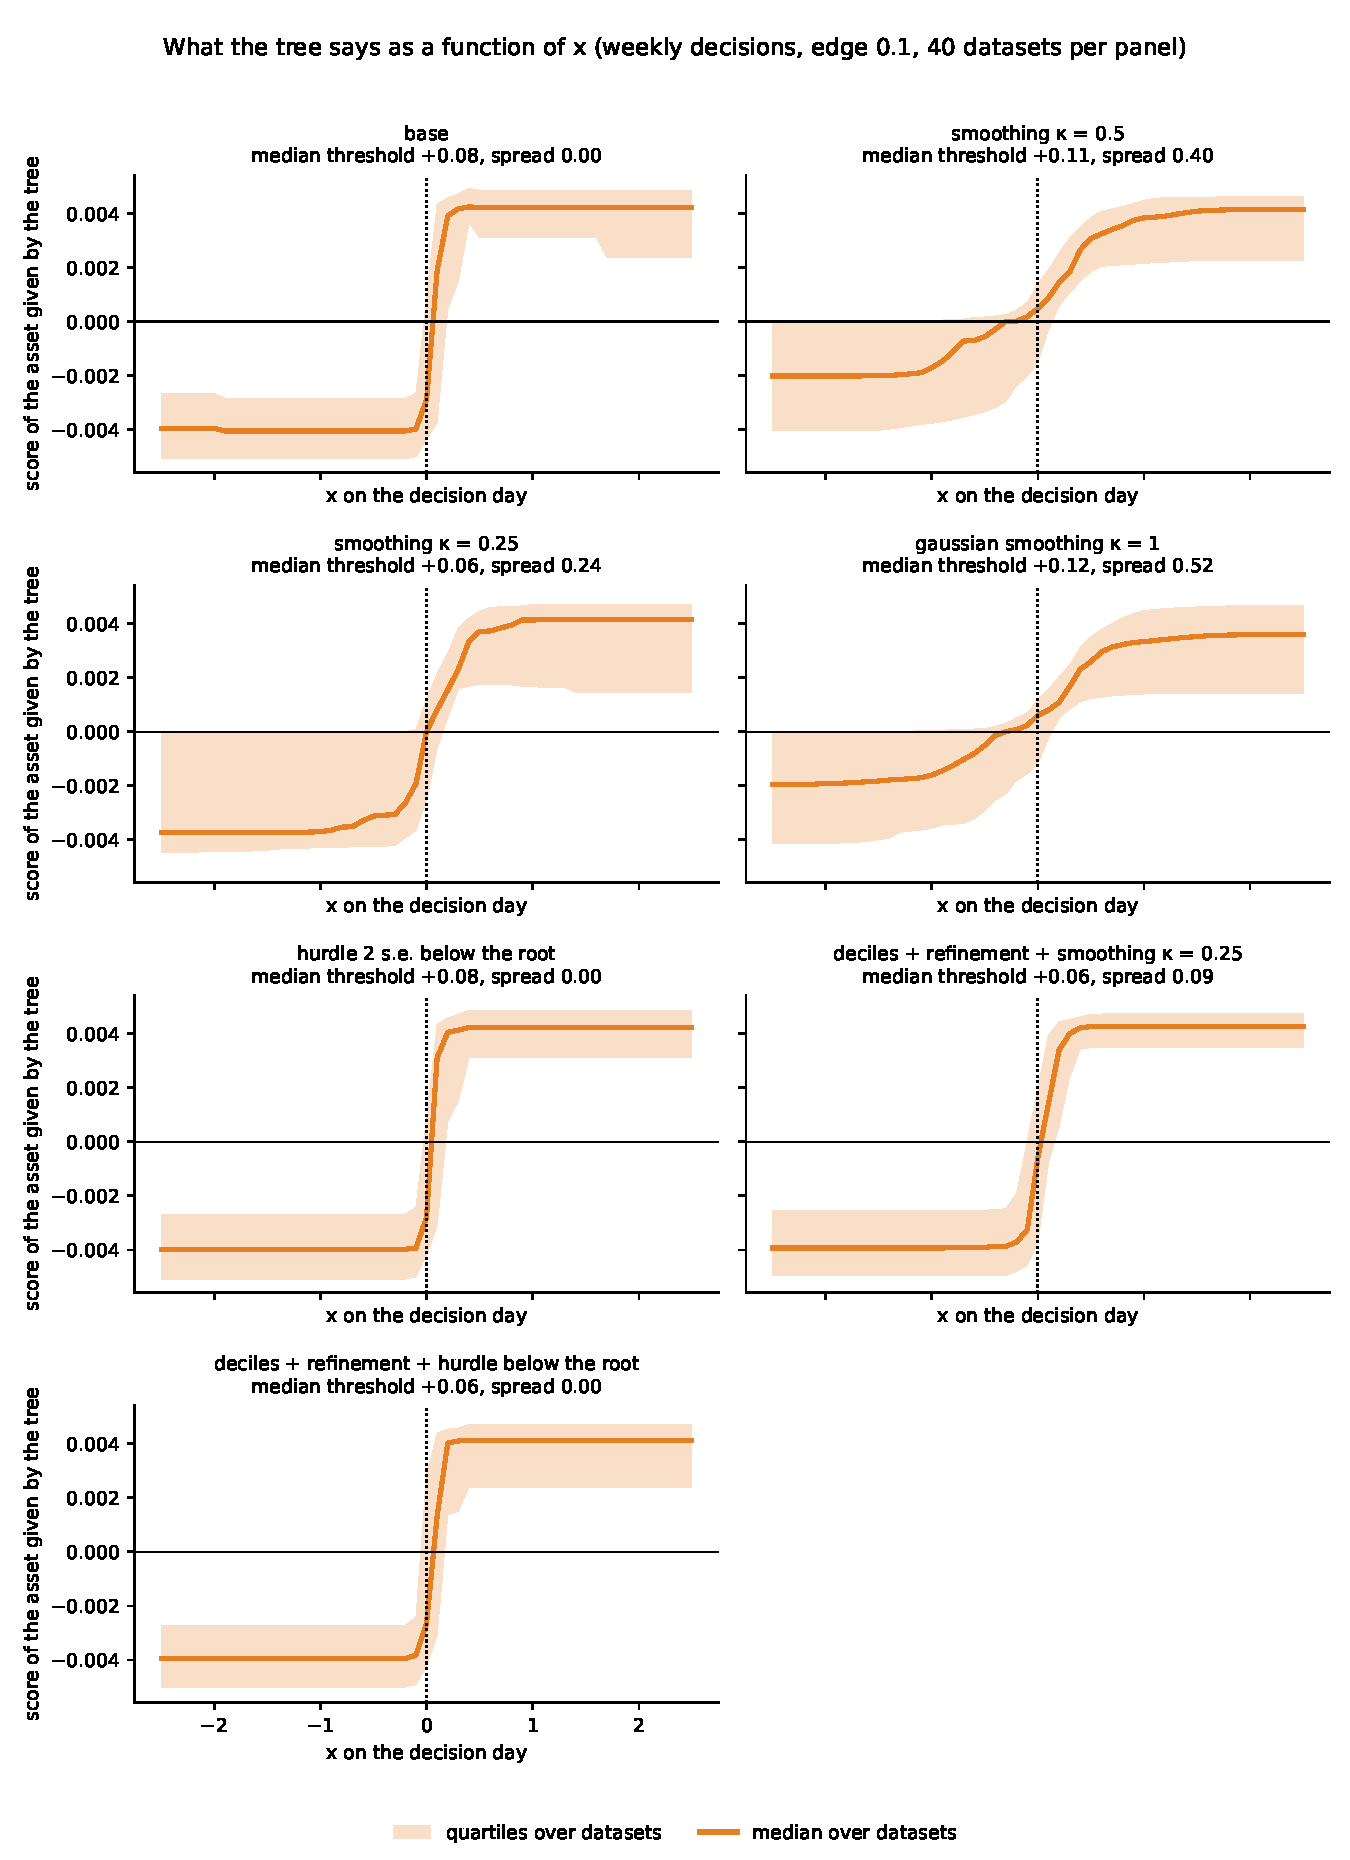
\includegraphics[width=0.9\linewidth]{split_options_2_scores}
\caption{Weekly decisions, edge 0.10: the score the tree gives the asset as a function of $x$ (median over the 40 datasets, quartiles as a band), one panel per setting.}
\label{fig:options2-scores}
\end{figure}
\begin{figure}[H]
\centering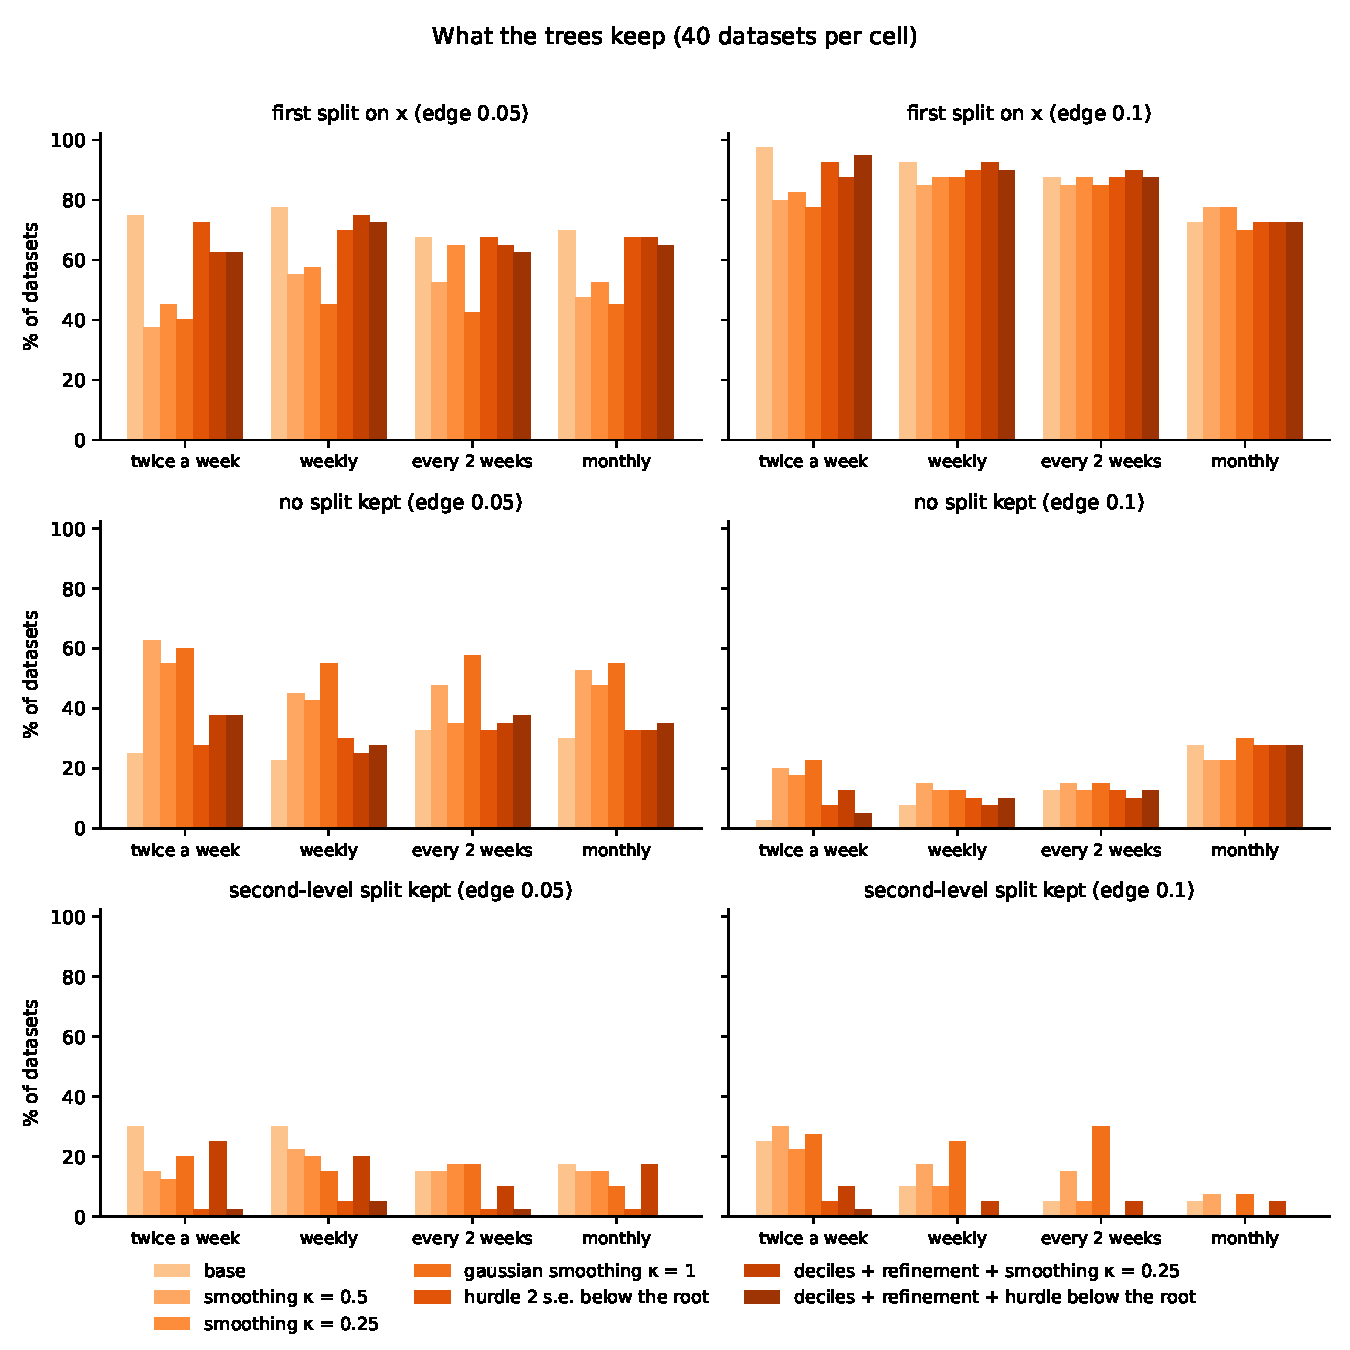
\includegraphics[width=0.9\linewidth]{split_options_2_splits}
\caption{What the trees keep, by setting and trading rate: first split on $x$, no split kept, a second-level split kept (\% of the datasets). \emph{Top:} edge 0.05; \emph{bottom:} edge 0.10.}
\label{fig:options2-splits}
\end{figure}
\begin{figure}[H]
\centering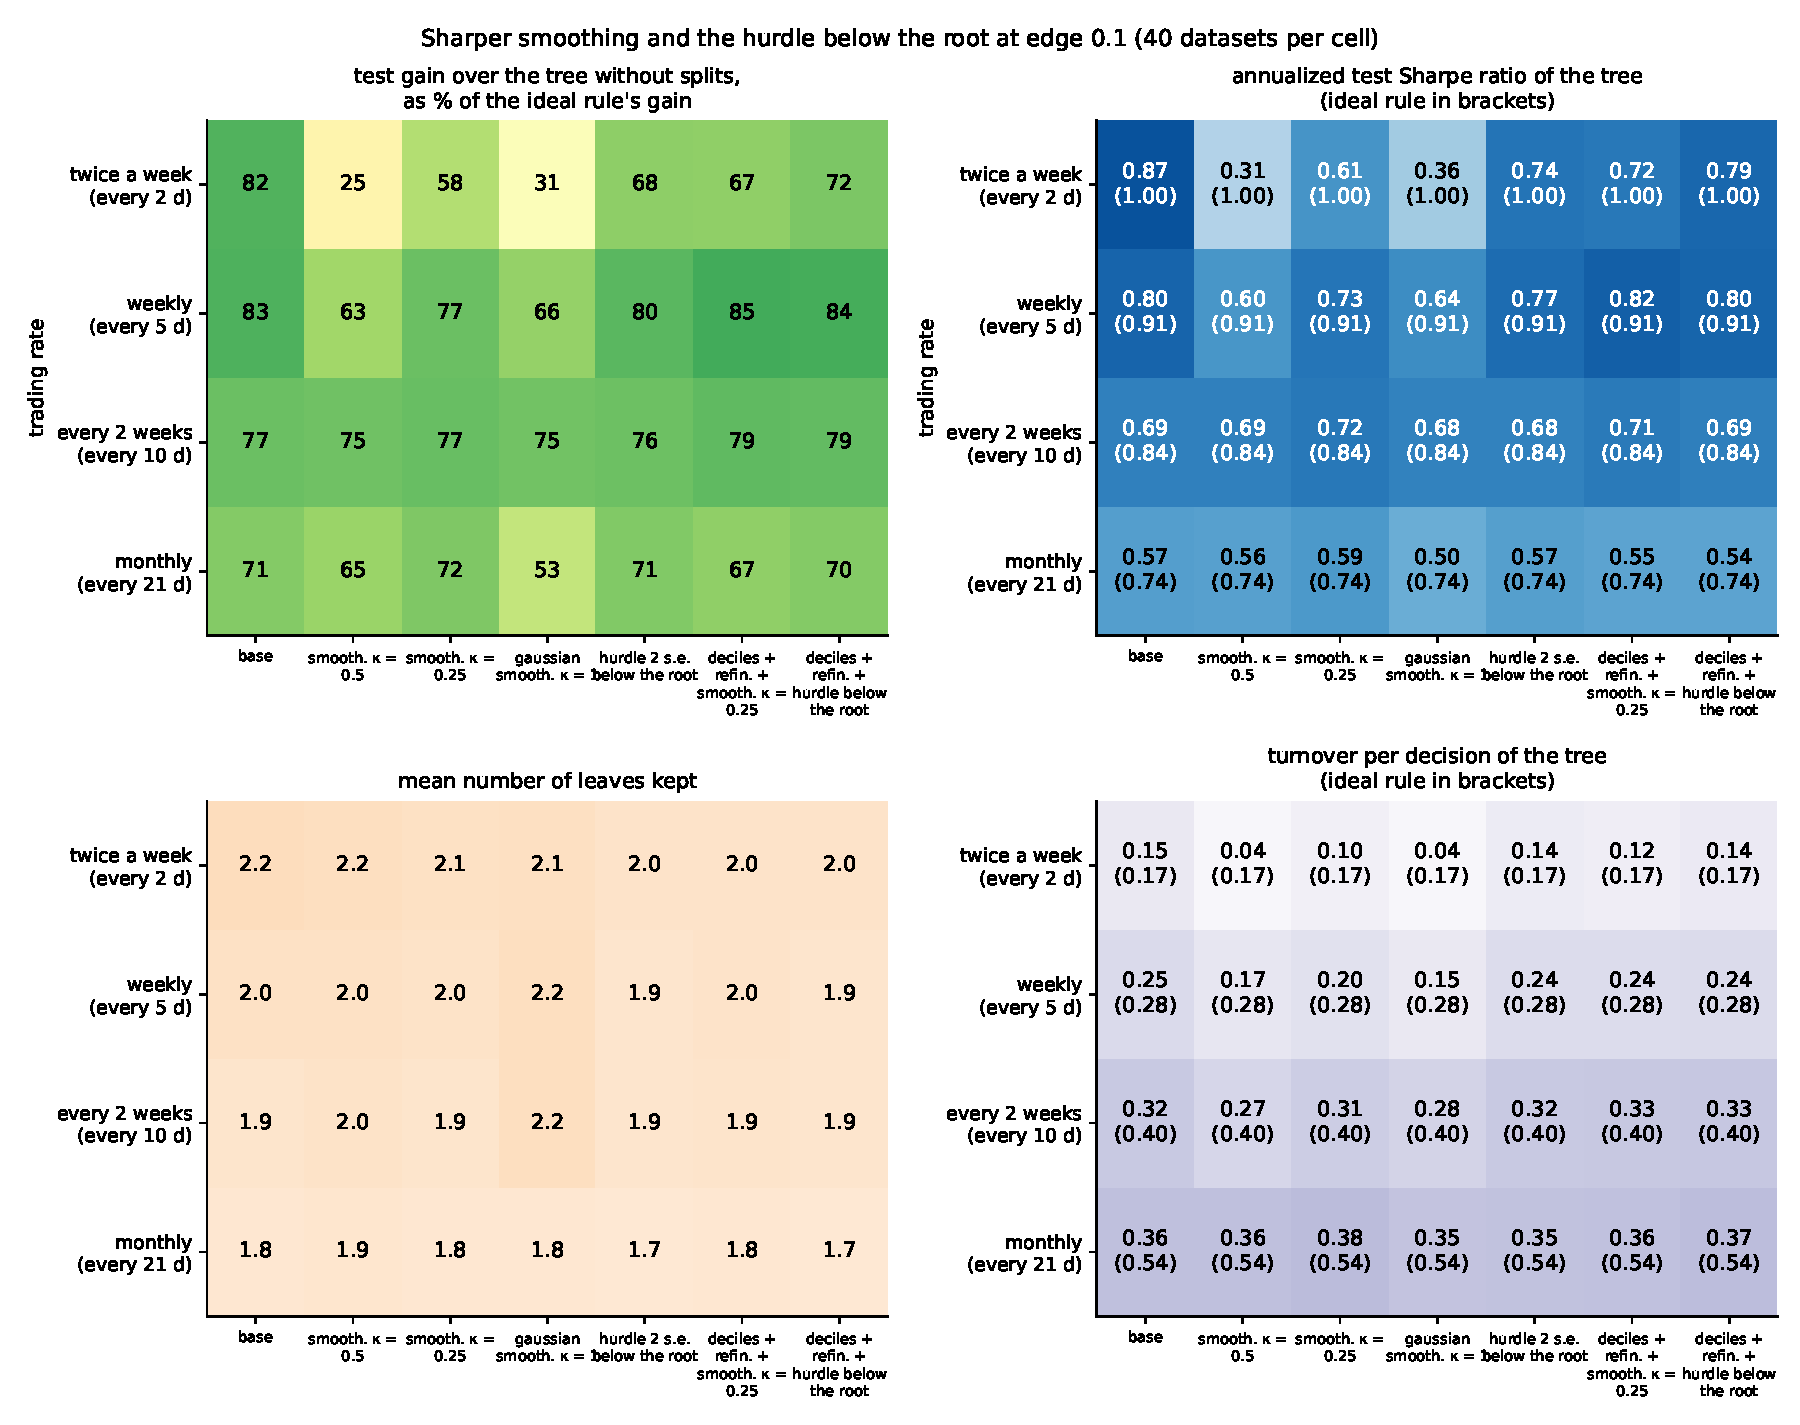
\includegraphics[width=0.95\linewidth]{split_options_2_maps}
\caption{Edge 0.10, rows: trading rate, columns: setting. Share of the ideal rule's test gain captured; annualized test Sharpe ratio (ideal rule in brackets); mean number of leaves; turnover per decision (ideal rule in brackets).}
\label{fig:options2-maps}
\end{figure}
\begin{figure}[H]
\centering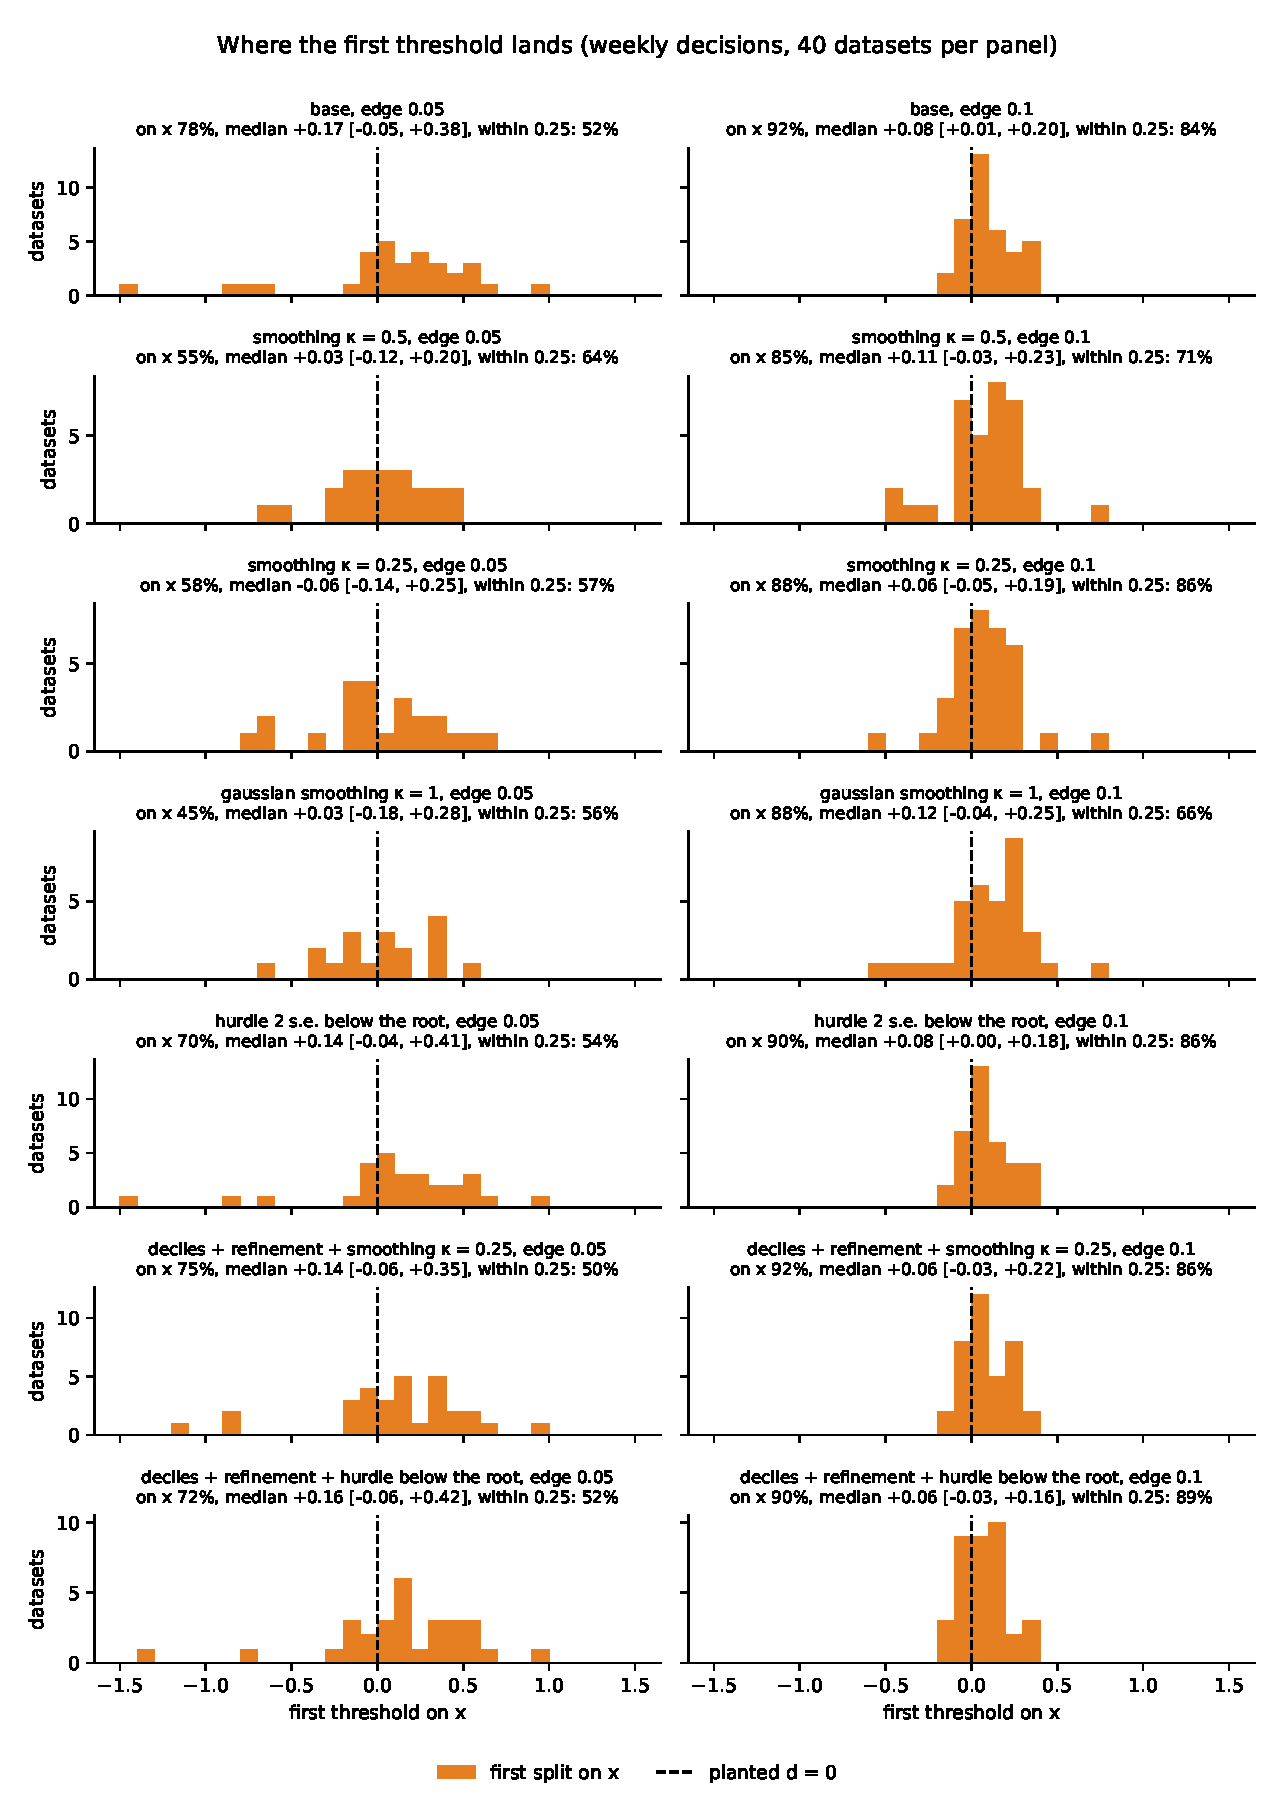
\includegraphics[width=0.9\linewidth]{split_options_2_thresholds}
\caption{Weekly decisions: where the first threshold lands, one row per setting; \emph{left:} edge 0.05, \emph{right:} edge 0.10.}
\label{fig:options2-thresholds}
\end{figure}

\begin{table}[H]
\centering\scriptsize
\setlength{\tabcolsep}{2.6pt}
\begin{tabular}{@{}l r rr r r r rr r r@{}}
\toprule
& & \multicolumn{2}{c}{datasets (\%)} & threshold & & 2nd & \multicolumn{2}{c}{annual.\ Sharpe} & gain & turn-\\
\cmidrule(lr){3-4}\cmidrule(lr){8-9}
setting & $h$ & on $x$ & none & $|\cdot|\le0.25$ & spread & level & tree & ideal & captured & over\\
\midrule
base & 2 & 98 & 2 & 97\% & -- & 25 & 0.87 & 1.00 & 82\% & 0.15\\
 & 5 & 92 & 8 & 84\% & -- & 10 & 0.80 & 0.91 & 83\% & 0.25\\
 & 10 & 88 & 12 & 63\% & -- & 5 & 0.69 & 0.84 & 77\% & 0.32\\
 & 21 & 72 & 28 & 45\% & -- & 5 & 0.57 & 0.74 & 71\% & 0.36\\
\midrule
smoothing $\kappa=0.5$ & 2 & 80 & 20 & 78\% & 0.37 & 30 & 0.31 & 1.00 & 25\% & 0.04\\
 & 5 & 85 & 15 & 71\% & 0.40 & 18 & 0.60 & 0.91 & 63\% & 0.17\\
 & 10 & 85 & 15 & 62\% & 0.45 & 15 & 0.69 & 0.84 & 75\% & 0.27\\
 & 21 & 78 & 22 & 74\% & 0.52 & 8 & 0.56 & 0.74 & 65\% & 0.36\\
\midrule
smoothing $\kappa=0.25$ & 2 & 82 & 18 & 85\% & 0.17 & 22 & 0.61 & 1.00 & 58\% & 0.10\\
 & 5 & 88 & 12 & 86\% & 0.24 & 10 & 0.73 & 0.91 & 77\% & 0.20\\
 & 10 & 88 & 12 & 60\% & 0.23 & 5 & 0.72 & 0.84 & 77\% & 0.31\\
 & 21 & 78 & 22 & 71\% & 0.37 & 0 & 0.59 & 0.74 & 72\% & 0.38\\
\midrule
Gaussian smoothing $\kappa=1$ & 2 & 78 & 22 & 68\% & 0.47 & 28 & 0.36 & 1.00 & 31\% & 0.04\\
 & 5 & 88 & 12 & 66\% & 0.52 & 25 & 0.64 & 0.91 & 66\% & 0.15\\
 & 10 & 85 & 15 & 65\% & 0.60 & 30 & 0.68 & 0.84 & 75\% & 0.28\\
 & 21 & 70 & 30 & 75\% & 0.66 & 8 & 0.50 & 0.74 & 53\% & 0.35\\
\midrule
hurdle 2 s.e.\ below the root & 2 & 92 & 8 & 97\% & -- & 5 & 0.74 & 1.00 & 68\% & 0.14\\
 & 5 & 90 & 10 & 86\% & -- & 0 & 0.77 & 0.91 & 80\% & 0.24\\
 & 10 & 88 & 12 & 63\% & -- & 0 & 0.68 & 0.84 & 76\% & 0.32\\
 & 21 & 72 & 28 & 45\% & -- & 0 & 0.57 & 0.74 & 71\% & 0.35\\
\midrule
deciles + refinement + smoothing $\kappa=0.25$ & 2 & 88 & 12 & 91\% & 0.10 & 10 & 0.72 & 1.00 & 67\% & 0.12\\
 & 5 & 92 & 8 & 86\% & 0.09 & 5 & 0.82 & 0.91 & 85\% & 0.24\\
 & 10 & 90 & 10 & 67\% & 0.08 & 5 & 0.71 & 0.84 & 79\% & 0.33\\
 & 21 & 72 & 28 & 59\% & 0.14 & 5 & 0.55 & 0.74 & 67\% & 0.36\\
\midrule
deciles + refinement + hurdle below the root & 2 & 95 & 5 & 87\% & -- & 2 & 0.79 & 1.00 & 72\% & 0.14\\
 & 5 & 90 & 10 & 89\% & -- & 0 & 0.80 & 0.91 & 84\% & 0.24\\
 & 10 & 88 & 12 & 71\% & -- & 0 & 0.69 & 0.84 & 79\% & 0.33\\
 & 21 & 72 & 28 & 55\% & -- & 0 & 0.54 & 0.74 & 70\% & 0.37\\
\bottomrule
\end{tabular}
\caption{Edge 0.10, 40 datasets per row ($h$: days between decisions). ``2nd level'': datasets that keep a second-level split; ``spread'': mean spread of the root split (soft splits); turnover per decision (the ideal rule's is 0.17, 0.28, 0.40 and 0.54). At edge 0.05 every smoothing setting loses most of the gain (Sharpe 0.06--0.20 against 0.19--0.27 for the base), the hurdle below the root equals the base (0.21, 0.27, 0.19, 0.26) with 2--5\% of second-level splits instead of 15--30\%, and deciles with refinement and the hurdle are within noise of the base.}
\label{tab:options2}
\end{table}

\textbf{Reading the figures and the table.}
\begin{itemize}\setlength{\itemsep}{1pt}
\item \textbf{Sharper weights cure the no-trade problem, not the loss.} At $\kappa=0.25$ the spread of the root split falls from 0.65 (Section~\ref{sec:enhancements}) to 0.17--0.37 and the turnover returns to the base level, so the score no longer sits in the optimizer's no-trade band. The tree then matches the base at weekly decisions and slower (0.73, 0.72, 0.59 against 0.80, 0.69, 0.57) with thresholds centred at least as well, but still loses 0.26 of Sharpe at every 2 days. $\kappa=0.5$ and the Gaussian form at $\kappa=1$ remain too wide (spreads 0.4--0.7) and behave like the $\kappa=1$ of Section~\ref{sec:enhancements}.
\item \textbf{On top of deciles with refinement, $\kappa=0.25$ gives the narrowest transition of all} (spread 0.08--0.14) and the best weekly numbers of the whole series, Sharpe 0.82 and 85\% of the gain, within noise of the base (0.80, 83\%); at every 2 days the soft edge still costs (0.72 against 0.87).
\item \textbf{The hurdle below the root does what the global hurdle could not.} Second-level splits fall from 25, 10, 5 and 5\% of the datasets to 5, 0, 0 and 0\%, the root splits are untouched (92, 90, 88, 72\% found against 98, 92, 88, 72), and from weekly decisions on the Sharpe ratio is unchanged (0.77, 0.68, 0.57 against 0.80, 0.69, 0.57). At edge 0.05 it also removes the second-level splits at no cost. At every 2 days it costs 0.13 of Sharpe: with 1{,}400 fitting decisions some second-level splits are real refinements, and the hurdle removes them with the noise.
\item \textbf{None of the options raises the Sharpe ratio above the base} beyond the noise of 40 datasets (standard error about 0.04). What they buy is steadier and better-centred thresholds at the slow rates and trees without spurious leaves. As defaults: the hurdle below the root from weekly decisions on, deciles with refinement for slow rates, and no smoothing unless positions are meant to be interior ($\lambda\ge5$).
\end{itemize}

\section{Model v1 on 100 datasets: the frozen configuration against the base}\label{sec:v1}
\textbf{Pipeline used.} P4 of \code{model_history.md} in the configuration frozen as \emph{model v1} on 24 September (section ``Configuration v1'' of \code{model_and_training_pipeline.tex}): depth at most 3, deciles by rank among the admissible thresholds with a 10\% leaf fraction, local refinement with a 1~s.e.\ hurdle, pruning hurdle of 2~s.e.\ below the root; every other parameter as in the base (plain pruning at the root, $\lambda=1$, fee 3~bp, 20 decisions per leaf, 180-day covariance); market M2. The base records are those of Section~\ref{sec:results} (P2, which is P4 with every option off) on the same datasets, seeds 0 to 99, so every comparison is paired.

\keybox{\textbf{In short.} Model v1 is the combination that Section~\ref{sec:options2} suggested (deciles with refinement and the hurdle below the root), with the depth raised to 3. Run as a whole on 100 datasets against the base of Section~\ref{sec:results} on the same datasets, it is \emph{the base within noise from weekly decisions on}: the paired differences of annualized test Sharpe are $0.00\pm0.04$, $+0.01\pm0.05$ and $-0.01\pm0.03$ at edge 0.10 (weekly, every 2 weeks, monthly) and $-0.03\pm0.05$, $+0.03\pm0.04$, $-0.03\pm0.03$ at edge 0.05, with the second-level leaves gone (18, 14 and 9\% of the datasets to 0, 2 and 0\% at edge 0.10) and trees of 1.9 leaves instead of 2.1. At every 2 days it costs $0.08\pm0.07$ at edge 0.10, as Section~\ref{sec:options2} had found on 40 datasets: some second-level splits are real there and the hurdle removes them. The depth budget of 3 is never used in this one-threshold market (at most 1\% of the trees reach the third level), so that choice is untested here. v1 is the base with a cleaner structure, not a higher Sharpe ratio.}

\textbf{Protocol.} The setting \code{V1} of \code{planted_threshold_experiments.py} (\code{run-v1}) fits model v1 on the datasets of seeds 0 to 99 at edges 0.05 and 0.10 and at the four trading rates of the option experiments, 800 fits; \code{plot} reads the base records of the same seeds, edges and rates from \code{results_daily_threshold.json} (800 of the 2{,}000 fits of Section~\ref{sec:results}) and compares them cell by cell and dataset by dataset. The paired difference is the annualized test Sharpe ratio of v1 minus that of the base on the same dataset; its standard error is that of the 100 differences. Because both trees are grown on the same rows, they often keep exactly the same root split (in 42 to 59\% of the datasets) and then give the same Sharpe ratio; the table counts these ties.

\begin{figure}[H]
\centering
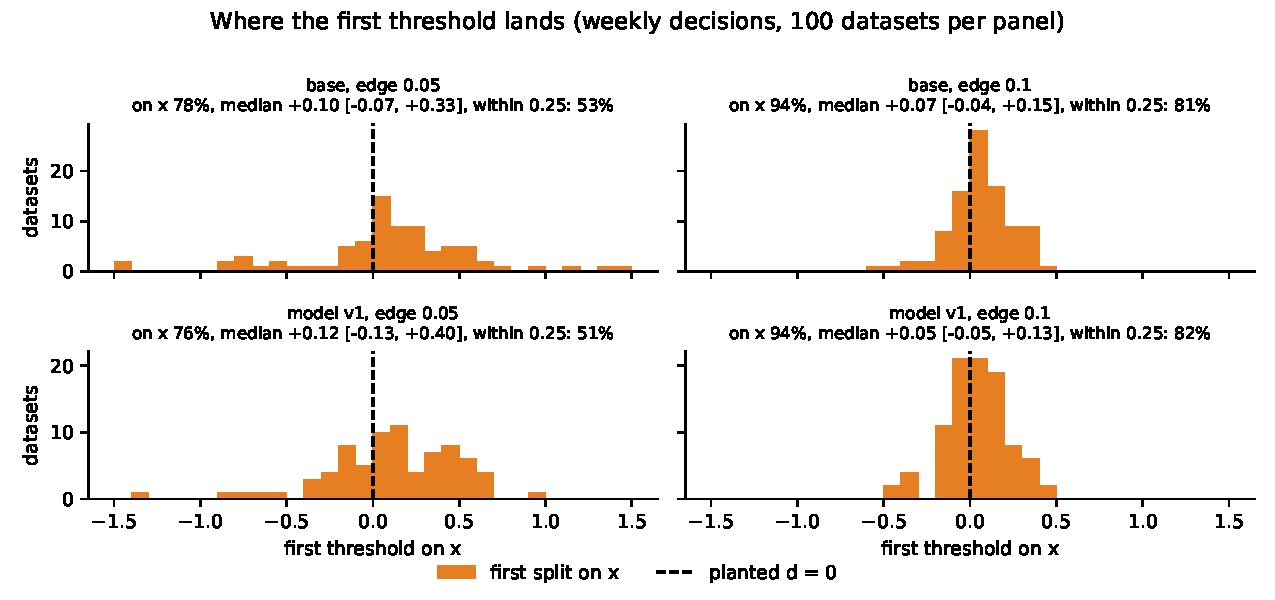
\includegraphics[width=0.8\linewidth]{model_v1_thresholds}
\caption{Where the first threshold lands, weekly decisions, 100 datasets per panel: the base (top) and model v1 (bottom), at edge 0.05 (left) and 0.10 (right).}
\label{fig:v1-thresholds}
\end{figure}

\begin{figure}[H]
\centering
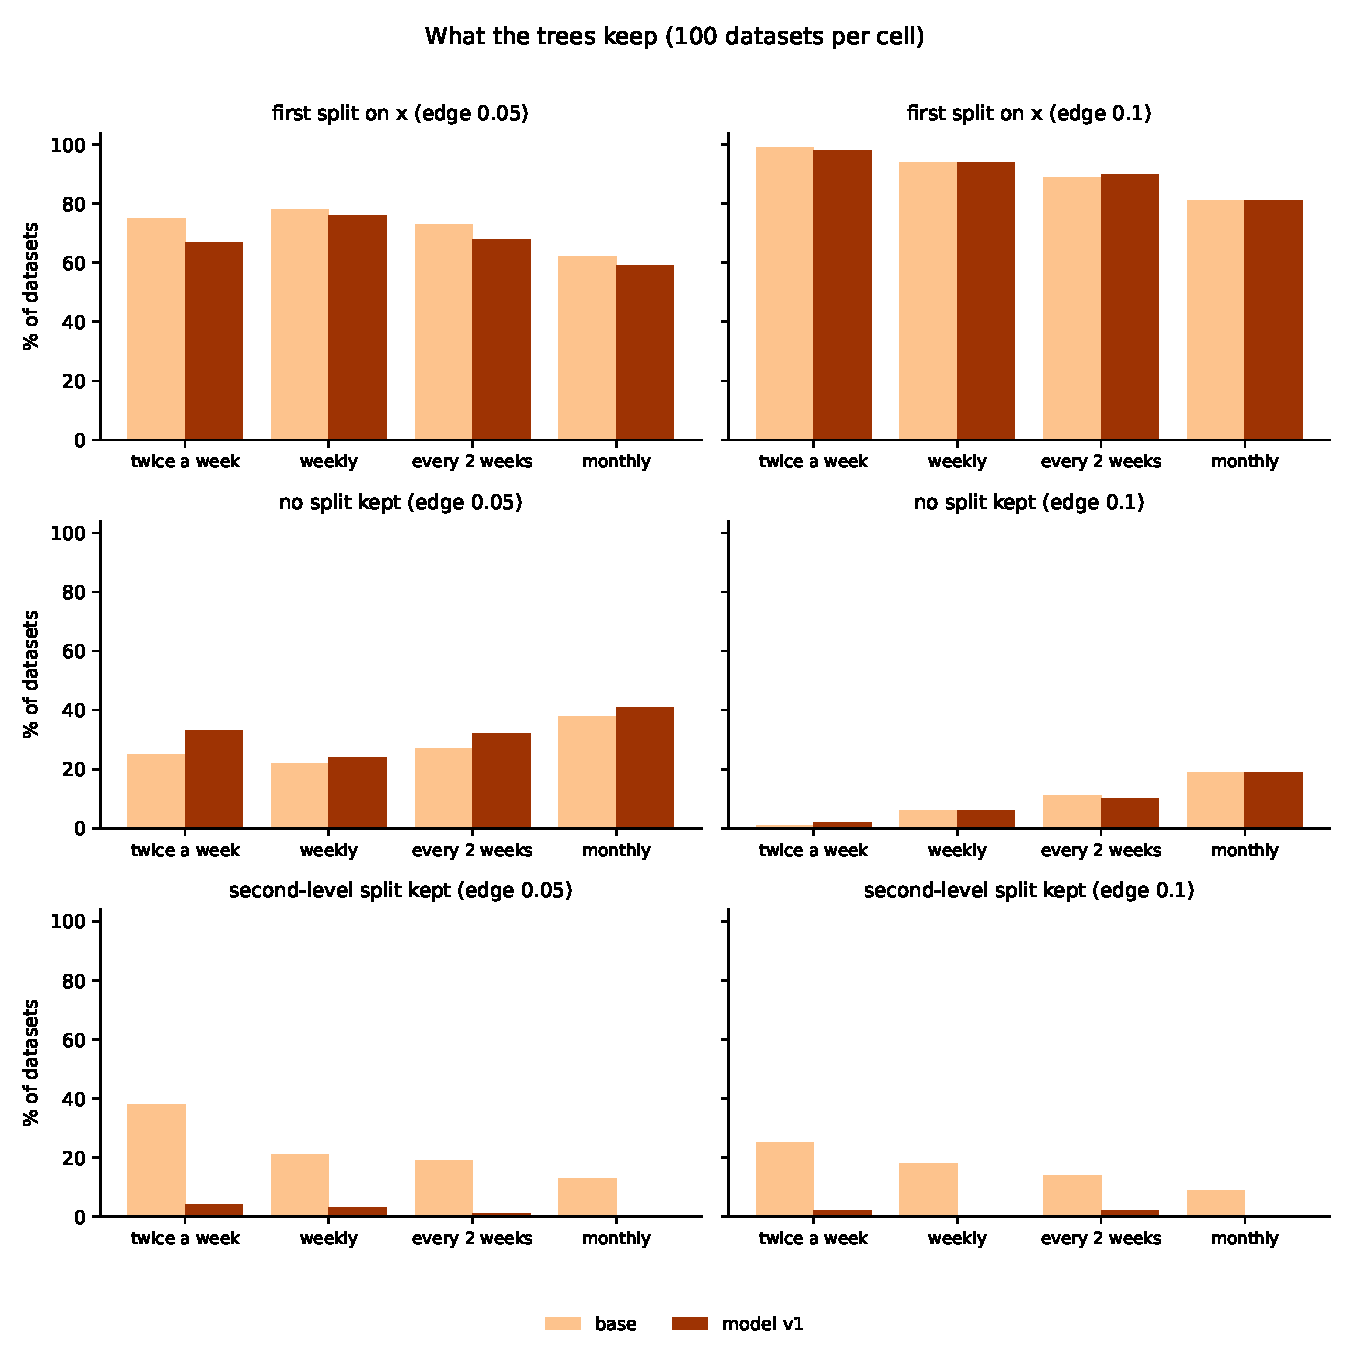
\includegraphics[height=0.46\textheight]{model_v1_splits}
\caption{What the trees keep, by rate: first split on $x$, no split kept, and a second-level split kept, base against v1, at both edges.}
\label{fig:v1-splits}
\end{figure}

\begin{figure}[H]
\centering
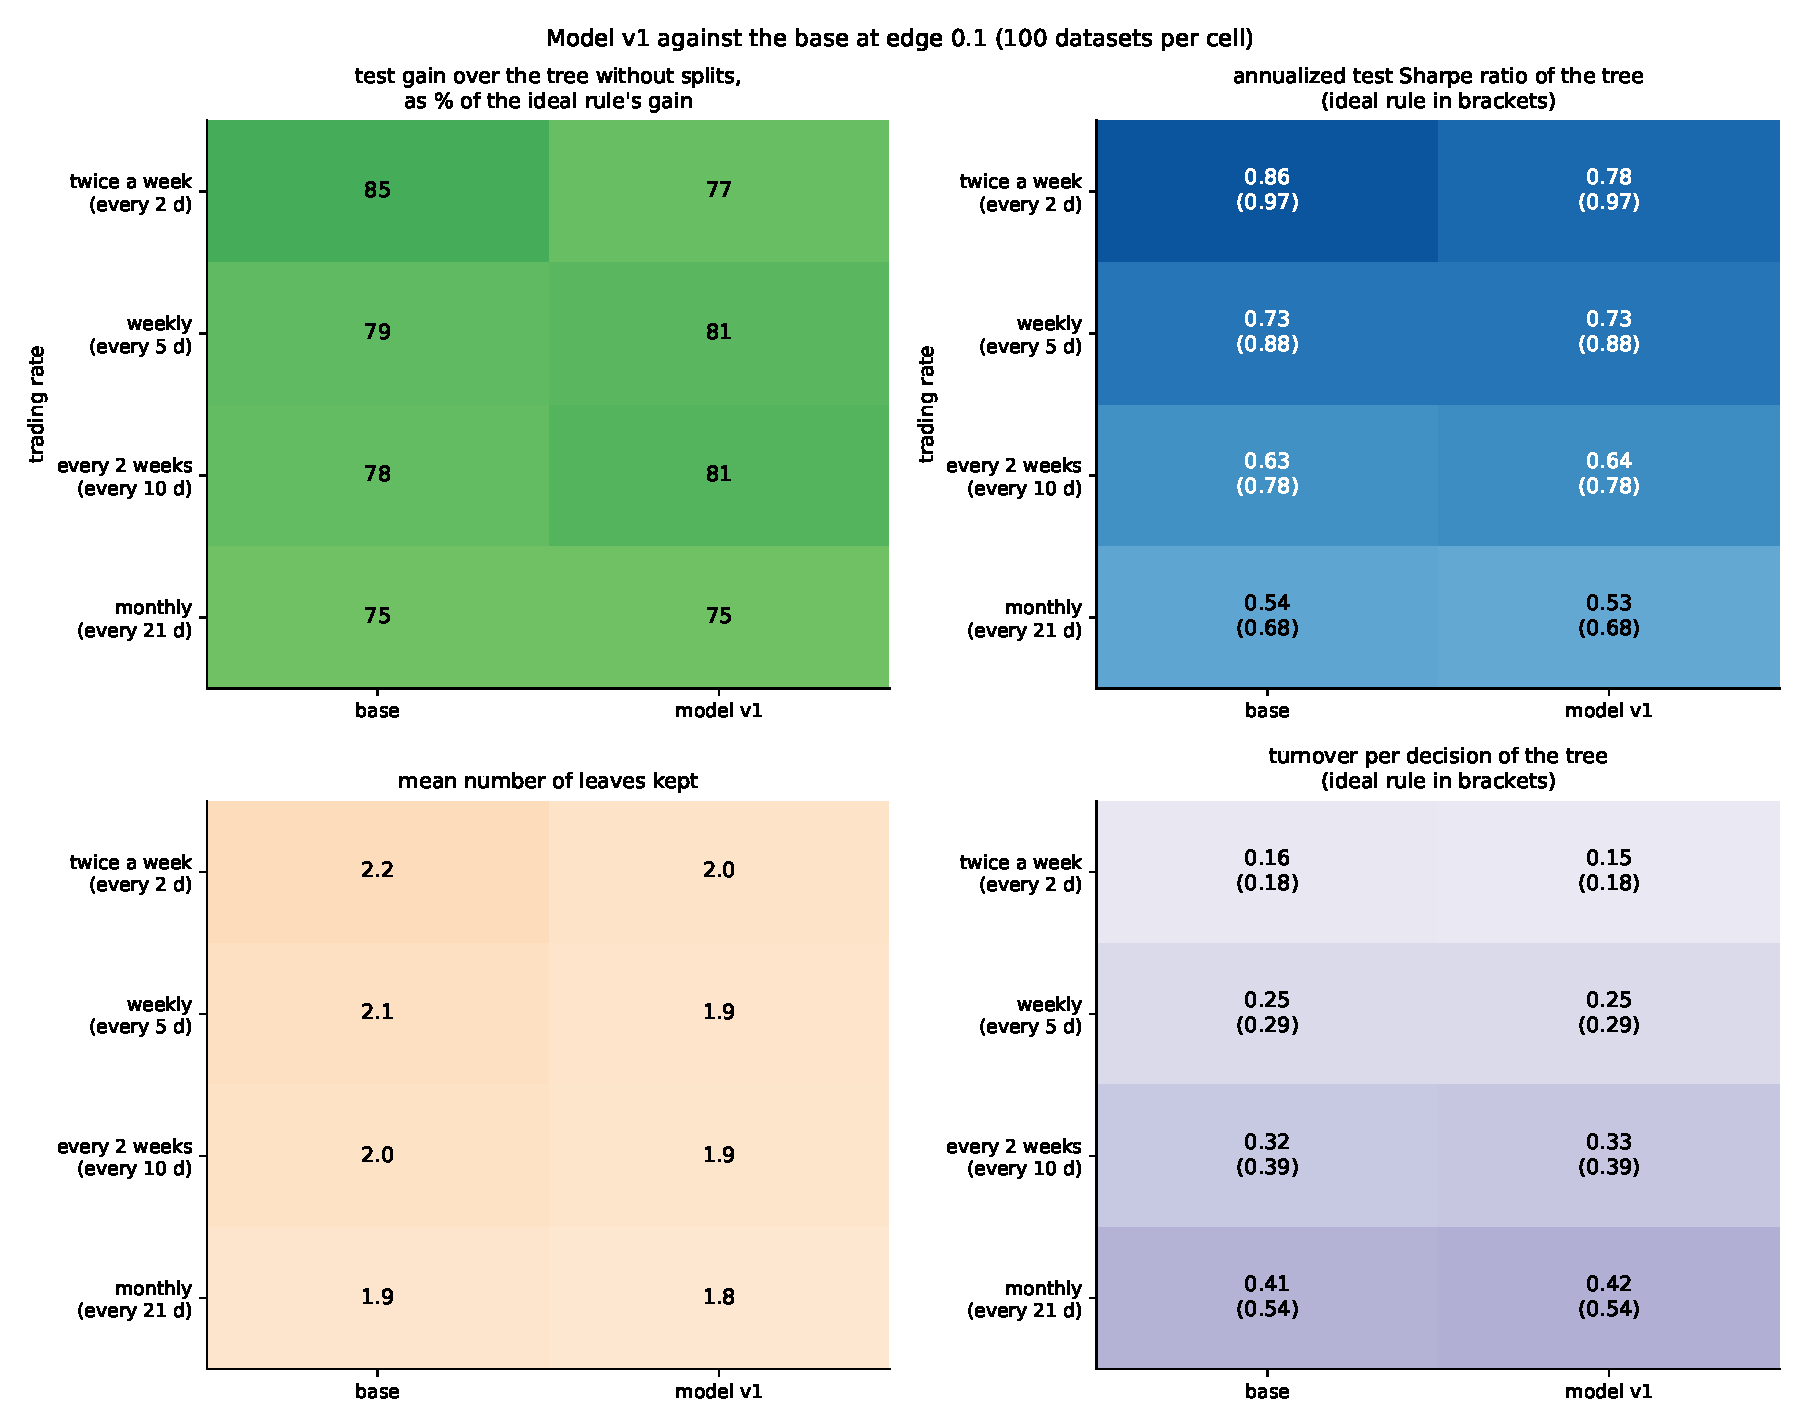
\includegraphics[width=0.9\linewidth]{model_v1_maps}
\caption{Model v1 against the base at edge 0.10: gain captured, Sharpe ratio, leaves kept and turnover, by trading rate.}
\label{fig:v1-maps}
\end{figure}

\begin{table}[H]
\centering\scriptsize
\setlength{\tabcolsep}{3pt}
\begin{tabular}{@{}l r r r l r r r r r r r@{}}
\toprule
& & & split & first threshold & & 2nd & \multicolumn{2}{c}{annual.\ Sharpe} & gain & v1 $-$ base & better /\\
\cmidrule(lr){8-9}
setting & $h$ & leaves & on $x$ & median [quartiles] & $|\cdot|\le0.25$ & level & tree & ideal & captured & (2 s.e.) & same / worse\\
\midrule
\multicolumn{12}{@{}l}{\emph{edge 0.10}}\\
base & 2 & 2.24 & 99 & $+0.03\ [-0.03,+0.11]$ & 92\% & 25 & 0.86 & 0.97 & 85\% & -- & --\\
 & 5 & 2.14 & 94 & $+0.07\ [-0.04,+0.15]$ & 81\% & 18 & 0.73 & 0.88 & 79\% & -- & --\\
 & 10 & 2.03 & 89 & $+0.07\ [-0.10,+0.21]$ & 70\% & 14 & 0.63 & 0.78 & 78\% & -- & --\\
 & 21 & 1.90 & 81 & $+0.06\ [-0.07,+0.25]$ & 60\% & 9 & 0.54 & 0.68 & 75\% & -- & --\\
model v1 & 2 & 2.00 & 98 & $+0.03\ [-0.04,+0.12]$ & 89\% & 2 & 0.78 & 0.97 & 77\% & $-0.08$ (0.07) & 20 / 52 / 28\\
 & 5 & 1.94 & 94 & $+0.05\ [-0.05,+0.13]$ & 82\% & 0 & 0.73 & 0.88 & 81\% & $+0.00$ (0.04) & 28 / 52 / 20\\
 & 10 & 1.92 & 90 & $+0.04\ [-0.15,+0.17]$ & 72\% & 2 & 0.64 & 0.78 & 81\% & $+0.01$ (0.05) & 20 / 48 / 32\\
 & 21 & 1.81 & 81 & $+0.03\ [-0.13,+0.22]$ & 64\% & 0 & 0.53 & 0.68 & 75\% & $-0.01$ (0.03) & 16 / 58 / 26\\
\addlinespace
\multicolumn{12}{@{}l}{\emph{edge 0.05}}\\
base & 2 & 2.18 & 75 & $+0.04\ [-0.12,+0.22]$ & 64\% & 38 & 0.21 & 0.46 & 44\% & -- & --\\
 & 5 & 2.01 & 78 & $+0.10\ [-0.07,+0.33]$ & 53\% & 21 & 0.24 & 0.43 & 51\% & -- & --\\
 & 10 & 1.93 & 73 & $+0.05\ [-0.20,+0.36]$ & 47\% & 19 & 0.17 & 0.39 & 43\% & -- & --\\
 & 21 & 1.76 & 62 & $+0.25\ [-0.06,+0.60]$ & 34\% & 13 & 0.17 & 0.35 & 43\% & -- & --\\
model v1 & 2 & 1.72 & 67 & $+0.05\ [-0.14,+0.24]$ & 57\% & 4 & 0.18 & 0.46 & 39\% & $-0.03$ (0.06) & 36 / 36 / 28\\
 & 5 & 1.80 & 76 & $+0.12\ [-0.13,+0.40]$ & 51\% & 3 & 0.22 & 0.43 & 49\% & $-0.03$ (0.05) & 35 / 42 / 23\\
 & 10 & 1.69 & 68 & $+0.11\ [-0.12,+0.38]$ & 49\% & 1 & 0.20 & 0.39 & 48\% & $+0.03$ (0.04) & 31 / 47 / 22\\
 & 21 & 1.59 & 59 & $+0.19\ [-0.10,+0.42]$ & 42\% & 0 & 0.14 & 0.35 & 42\% & $-0.03$ (0.03) & 17 / 57 / 26\\
\bottomrule
\end{tabular}
\caption{Model v1 against the base on the same 100 datasets ($h$: days between decisions). ``Leaves'': mean number of leaves kept; ``2nd level'': share of datasets that keep a second-level split; ``v1 $-$ base'': mean paired difference of the annualized test Sharpe ratio, with twice its standard error; ``better / same / worse'': share of datasets where v1's Sharpe ratio is above, equal to, or below the base's. With one feature, the datasets that do not split on $x$ keep no split.}
\label{tab:v1}
\end{table}

\textbf{Reading the figures and the table.}
\begin{itemize}\setlength{\itemsep}{1pt}
\item \textbf{From weekly decisions on, v1 is the base.} The paired differences are within twice their standard error at every rate and both edges (largest: $\pm0.03$), and in half of the datasets the two trees give exactly the same Sharpe ratio. The gain captured is the same to a few points (79 to 81\% weekly, 78 to 81\% every 2 weeks, 75\% monthly at edge 0.10).
\item \textbf{The second-level leaves are gone and the thresholds are as well centred.} At edge 0.10 the share of datasets with a second-level split falls from 25, 18, 14 and 9\% to 2, 0, 2 and 0\%; the root split is found as often (98, 94, 90, 81\% against 99, 94, 89, 81) and within 0.25 of $d$ as often or more (89, 82, 72, 64\% against 92, 81, 70, 60); the trees keep 1.9 leaves instead of 2.1. At edge 0.05 the same holds for the second level (38, 21, 19, 13\% to 4, 3, 1, 0\%), and the root is found a little less often (67, 76, 68, 59\% against 75, 78, 73, 62): with a weak signal the decile candidates sometimes miss the split the full screen finds, as Section~\ref{sec:enhancements} had noted.
\item \textbf{Every 2 days, v1 costs $0.08\pm0.07$ at edge 0.10} (v1 better in 20\% of the datasets, worse in 28\%) and the gain captured falls from 85 to 77\%. With 1{,}400 fitting decisions a quarter of the base trees keep a real second-level refinement and the hurdle removes it with the noise, as in Section~\ref{sec:options2}. At edge 0.05 the 2-day difference is $-0.03\pm0.06$. For the 2-day alternative of v1 the hurdle should be softer (1~s.e.\ below the root) or off; this was not run.
\item \textbf{The depth budget is not used.} v1 grows trees of 3 to 4 leaves and prunes them to 1.6 to 2.0; a split at the third level survives in at most 1\% of the datasets. In a market with one threshold the maximum depth of 3 changes nothing, as Section~\ref{sec:settings} had found for the base; whether it helps with two features and an interaction is the next experiment's question.
\item \textbf{At edge 0.05 and monthly decisions the difference is $-0.03\pm0.03$}, at the edge of noise: with 180 training decisions the hurdle has removed second-level splits from 13\% of the trees and the deciles have cost three root splits; the base itself finds the threshold in only 62\% of these datasets.
\end{itemize}

\textbf{What this says.} The 100-dataset paired test confirms what the 40-dataset experiments suggested: v1 is not a higher Sharpe ratio, it is the same Sharpe ratio with smaller trees, thresholds as well centred, ten times fewer candidates screened, and no spurious leaf, from weekly decisions on. Its known cost is at every 2 days. The parts of v1 that this market cannot test are the depth budget and the behaviour with several features; the part it does not question is the growth gate on the replayed Sharpe ratio, kept as designed.

\section{How to reproduce}
The code is in \code{code/} (run the commands below from that folder, with the project's Python, \code{../.venv/bin/python}); results and figures are in \code{report/figures/}. The results were produced with \code{synthetic_market.py} as committed in \code{eae145c} (one volatility for both regimes).
\begin{itemize}\raggedright\setlength{\itemsep}{1pt}
\item \code{python planted_threshold_test.py}: one dataset, printed in detail (about 10 s).
\item \code{python planted_threshold_experiments.py} \code{run}: the 2{,}000 fits in parallel, 103 minutes on 10 cores; writes \code{results_daily_threshold.json}.
\item \code{python planted_threshold_experiments.py} \code{plot}: the figures and the summary table of Tables~\ref{tab:edge}--\ref{tab:k}.
\item \code{python -m unittest discover -s tests}: 64 tests, including the alignment and no-look-ahead checks of the rows, the Sharpe-of-cash convention and the split-search and pruning options.
\item \code{python planted_threshold_experiments.py} \code{run-settings}: the settings experiment of Section~\ref{sec:settings}, 1{,}920 fits, 54 minutes; writes \code{results_risk_fee_depth.json}, which \code{plot} then turns into Figures~\ref{fig:positions}--\ref{fig:settings-maps} and Table~\ref{tab:settings}.
\item \code{python planted_threshold_experiments.py} \code{run-enhancements}: the split-search options of Section~\ref{sec:enhancements}, 1{,}600 fits, 35 minutes; writes \code{results_split_options.json}, drawn by \code{plot} as Figures~\ref{fig:scores}--\ref{fig:enh-maps} and Table~\ref{tab:enhancements}.
\item \code{python planted_threshold_experiments.py} \code{run-pruning}: the pruning hurdle of Section~\ref{sec:pruning}, 1{,}600 fits, 30 minutes; writes \code{results_pruning_hurdle.json}, drawn by \code{plot} as Figures~\ref{fig:pruning-splits}--\ref{fig:pruning-thresholds} and Table~\ref{tab:pruning}.
\item \code{python planted_threshold_experiments.py} \code{run-resolution}: the resolution sweeps of Section~\ref{sec:resolution}, 1{,}920 fits; writes \code{results_resolution.json}, drawn by \code{plot} as Figure~\ref{fig:resolution}.
\item \code{python planted_threshold_experiments.py} \code{run-options}: the sharper smoothing weights and the hurdle below the root of Section~\ref{sec:options2}, 2{,}240 fits; writes \code{results_split_options_2.json}, drawn by \code{plot} as Figures~\ref{fig:options2-scores}--\ref{fig:options2-thresholds}.
\item \code{python planted_threshold_experiments.py} \code{run-v1}: model v1 on 100 datasets (Section~\ref{sec:v1}), 800 fits; writes \code{results_model_v1.json}, which \code{plot} compares with the base records of \code{results_daily_threshold.json} (Figures~\ref{fig:v1-thresholds}--\ref{fig:v1-maps} and Table~\ref{tab:v1}).
\item \code{report/model_and_training_pipeline.tex}: the model and its training, step by step, with the equations of every option.
\end{itemize}
\end{document}
